 \documentclass{article}

% Language setting
% Replace `english' with e.g. `spanish' to change the document language
\usepackage[german]{babel}
\usepackage{pgfplots}
% Set page size and margins
% Replace `letterpaper' with `a4paper' for UK/EU standard size
\usepackage[letterpaper,top=2cm,bottom=2cm,left=3cm,right=3cm,marginparwidth=1.75cm]{geometry}
\usepackage{tabularx}
\usepackage{listings}
\lstset{
  basicstyle=\fontfamily{lmvtt}\selectfont\small\color{blue},
  columns=fullflexible,
}

% Useful packages
\usepackage{amsmath}
\usepackage{amssymb}
\usepackage{graphicx}
\usepackage[colorlinks=true, allcolors=blue]{hyperref}
\usepackage{tkz-euclide}
\usepackage{titlesec}
\usepackage{tikz}
\DeclareUnicodeCharacter{2212}{−}
\usepgfplotslibrary{groupplots,dateplot}
\usetikzlibrary{patterns,shapes.arrows}
\pgfplotsset{compat=newest}
\usepackage[utf8]{inputenc}
\usepackage{esvect}
\usepackage{caption}
\DeclareCaptionLabelFormat{blank}{}
\usepackage{animate}

\usepackage{siunitx}
\usepackage{fp}
\usetikzlibrary{scopes, decorations.pathmorphing}

\author{Valentino Gaber}
\begin{document}
\begin{center}
    \Large{Bewegte Objekte in der speziellen Relativitätstheorie}
\end{center}
\begin{center}
    \large{Betreut durch Herr Röthlisberger}
\end{center}
\begin{center}
    \Large Valentino Gaber \\
    \vspace{0.4cm}
    \large 1. Februar 2023\\
    \vspace{0.7cm}
    \Large Maturaarbeit \\
    \Large in\\
    \Large Physik
\end{center}
\begin{figure}[h]
    \centering
    \begin{tikzpicture}

% This command generates a Minkowski space diagram.
% 
% Parameter 1: width of 1 grid space
% Parameter 2: maximum x/ct value
% Parameter 3: proportion of speed of light
\newcommand{\spacetimediagram}[3]{
    % Draw the x and ct axes
    \draw[<->,thick] (-#2*#1-#1, 0) -- (#2*#1+#1, 0);
    \draw[<->,thick] (0, -#2*#1-#1) -- (0, #2*#1+#1);
    % Draw the x ct grid
    \draw[step=#1,gray,very thin] (-#2*#1, -#2*#1) grid (#2*#1, #2*#1);

    % Evaluate the Lorentz transformation
    \FPeval{\calcgamma}{1/((1-(#3)^2)^.5)}
    \FPeval{\calcbetagamma}{\calcgamma*#3}

    % Draw the x' and ct' axes
    \draw[<->,thick,cm={\calcgamma,\calcbetagamma,\calcbetagamma,\calcgamma,(0,0)},blue] (-#2*#1-#1, 0) -- (#2*#1+#1, 0);
    \draw[<->,thick,cm={\calcgamma,\calcbetagamma,\calcbetagamma,\calcgamma,(0,0)},blue] (0, -#2*#1-#1) -- (0, #2*#1+#1);

    % Draw the vertical transformed grid lines
    \foreach \x in {-#2,...,#2}
        \draw[cm={\calcgamma,\calcbetagamma,\calcbetagamma,\calcgamma,(0,0)},blue,very thin] (\x*#1,-#2*#1) -- (\x*#1,#2*#1);
    % Draw the horizontal transformed grid lines
    \foreach \y in {-#2,...,#2}
        \draw[cm={\calcgamma,\calcbetagamma,\calcbetagamma,\calcgamma,(0,0)},blue,very thin] (-#2*#1,\y*#1) -- (#2*#1,\y*#1);

    % Draw the x and ct axes labels
    \draw (#2*#1+#1+0.2,0) node {$x$};
    \draw (0,#2*#1+#1+0.2) node {$ct$};
    % Draw the x' and ct' axes labels
    \draw[cm={\calcgamma,\calcbetagamma,\calcbetagamma,\calcgamma,(0,0)},blue] (#2*#1+#1+0.2,0) node {$x^\prime$};
    \draw[cm={\calcgamma,\calcbetagamma,\calcbetagamma,\calcgamma,(0,0)},blue] (0,#2*#1+#1+0.2) node {$ct^\prime$};
    
    % Draw the unit indicators
}
\spacetimediagram{.5}{8}{1/2}
\end{tikzpicture}
\end{figure}
\vspace{-1cm}
\begin{center}
    
\end{center}

\newpage
\begin{abstract}
    Diese Arbeit wurde im Rahmen der Maturaarbeit erstellt. Sie handelt von den mathematischen und physikalischen Hintergründen und deren Anwendungen der speziellen Relativitätstheorie. Es werden Phänomen wie Zeitdilatation, Längenkontraktion und relativistischer Doppler-Effekt behandelt und es wird eine Einleitung in die mathematischen Hintergründe, wie 4er-Vektoren, Lorentz-Transformationen und Minkowski Diagramme, gewährt. Aufgrund dieses Wissens wird eine Simulation erstellt zur Veranschaulichung der Effekte auf die visuelle Wahrnehmung von Objekten bei relativistischen Geschwindigkeiten. Es wird zusammen mit dem Leser die Erstellung des Codes durchgeführt und es wird ein Einblick in die numerischen Methoden, der im Code verwendeten Gleichungen eingegangen. Man kommt zum Schluss, dass sich die Objekte nicht verhalten, wie man aus den Gleichungen schlussfolgern würde. Anstatt von reinen Längenkontraktionen werden sogenannte Terrell Rotationen beobachtet. 
\end{abstract}

\newpage
\tableofcontents
\newpage

\section{Einleitung}
\subsection{Wieso habe ich mir dieses Themengebiet ausgesucht?}
Diese Frage ist einfach zu beantworten, da ich mich sehr für schwarze Löcher und den Kosmos mit all seinen Tücken und Zügen interessiere und darum ist die Relativitätstheorie grundlegend für jegliche Beobachtungen. Ich wollte schon lange eine Arbeit über Schwarze Löcher schreiben. Man sollte mit den mathematischen sowie physikalischen Grundlagen vertraut sein, um die Aspekte und Auswirkung auf ihre unmittelbare Umgebung und den Kosmos zu erforschen.

Die Relativitätstheorie ist, wie schon erwähnt, grundlegend für die Forschung in jenem Themenbereich. Die Relativitätstheorie, wie sich Objekte bei den höchsten irdischen Geschwindigkeiten bis hin zur Lichtgeschwindigkeit im Vakuum bewegen. Dabei merkt man schnell, dass sich Beobachtungen abhängig vom Beobachter unterschiedlich verhalten. Nun stellt man fest, dass sich jene Beobachtungen von System zu System mittels einer Gleichung umformen lassen, von Beobachter zu Beobachter und dass alle Ergebnisse den Gesetzen der Physik folgen und ineinander transformierbar sind (Annahmen für die spezielle Relativitätstheorie).

Dies ist genau das Faszinierende für mich. Egal in welchem System man sich befindet, trifft man meistens dieselben physikalischen Gesetze an. Ebenfalls fasziniert mich die breite Anwendbarkeit der Relativitätstheorie. Man trifft sie nicht nur in der Astrophysik, sondern auch in heutzutage selbstverständlichen Dingen wie dem GPS an. Ohne die Relativitätstheorie wären die Angaben des GPS um einige Kilometer ungenauer und man könnte dem GPS nicht vertrauen. Dank Einstein weiss man wieso die Uhren auf Satelliten um 38 ns schneller laufen als hier auf der Erde. Wenn man die 38 ns nicht berücksichtigen würde, könnten all unsere Navigationssysteme nicht funktionieren. 

Die Relativitätstheorie ist nicht nur wichtig für das GPS, wenn man an die Anwendung von Einsteins Theorie denkt. Man kann sie in zahlreichen anderen Geräten anwenden, bspw. in CRTs (cathode-ray-tubes), diese finden sich in alten Fernsehern, welche zugegebenermassen veraltet sind, ohne jene wir jedoch die Geräte welche wir heute haben nicht erfunden hätten. Andere Anwendung findet sie in modernerer Technologie wie LIDAR und Doppler Radar. Dabei sind die Berechnungen für die Laser Länge abhängig vom relativistischen Verhalten von Licht. Natürlich findet sich der Doppler-Effekt unabhängig vom Licht in der Natur wieder, bspw. in Wellen. 

Jeder hat schon mal vom Doppler-Effekt von Wellen entweder in der Wellenlehre oder im Alltag gehört. Den Doppler-Effekt von Klang-Wellen trifft man z.B. bei Krankenwagen an, wenn sie mit der Sirene vorbeifahren. Obwohl der Doppler-Effekt für Licht und für Klang den selben Namen trägt unterscheiden sich die Berechnungen der beiden massgebend und können somit nicht mit denselben Gleichungen beschrieben werden. Hier kommt nun wieder die Relativitätstheorie zum Zuge, spezifisch die Spezielle Relativitätstheorie. Nebst all jenen Erfindungen und Beobachtungen vergisst man oft, dass die berühmte Gleichung $E = mc^2$ eigentlich aus der speziellen Relativitätstheorie herleitbar ist und man mit jener eine ganz neue Welt von Gleichungen und Anwendungen entdeckt. Namentlich die Atom-Bombe, ohne jene kleine Gleichung und somit ohne die spezielle Relativitätstheorie wäre die Atom-Bombe nicht denkbar gewesen. Neben der Atom Bombe sind die friedlich genutzten Kernreaktoren auch basierend auf Einsteins weltbekannter Gleichung. Nebst den Anwendungen der Stromgewinnung findet sich die Gleichung in der Medizin wieder, namentlich in PET Scans (positron emission tomography).

Nun wie schon zuvor ausgeführt fasziniert mich die Vielseitigkeit dieser Theorie und insbesondere deren Anwendung für kosmische Objekte, wie schwarze Löcher.

\subsection{Was ist das Ziel meiner Arbeit?}
Das ist eine Frage die sich erst im Verlauf des Projekts beantworten lässt. Mein Ziel war es anfangs etwas mit Schwarzen Löchern zu machen, dazu musste man jedoch erstmals die Relativitätstheorie richtig gut beherrschen um später die Schwarzschild-Metrik und die Rechnungen mit jener beweisen und verstehen zu können. Herr Röthlisberger brachte mich schnell wieder auf den Boden der Tatsachen zurück und wir beschlossen erstmals eine saubere Arbeit in der speziellen Relativitätstheorie zu machen und wenn noch Zeit übrig ist, einen kleinen Exkurs in die allgemeine Relativitätstheorie und Schwarze Löcher zu machen. Mir wurde schnell klar, dass ich Simulationen machen muss. Da ich von Anfang an eine eher theoretische Arbeit schreiben wollte, war dies kein Problem für mich. Das Ziel meiner Arbeit ist eine Beschreibung sowie Darstellung der Relativitätstheorie mit Anwendung mittels einer Python-Simulation und der somit verbundenen Analyse der durch die Python-Simulationen erfahrenen Beobachtungen, welche sich mit deren numerischen Anwendung der theoretischen Gleichungen per Hand decken sollten.



\section{Klassische Transformationen}
\subsection{Galilei Transformation}
\subsubsection{Was sind Galilei Transformationen?}
Als Galilei-Transformationen werden Transformationen bezeichnet, welche die Koordinaten von einem Inertialsystem ins nächste übertragen. Unter der Bedingung, dass das Inertialsystem unbeschleunigt ist und das sich die beiden Koordinatensysteme mit konstanter Geschwindigkeit zu einander bewegen. Die Galilei-Transformation ist zentral für die klassische Mechanik. In der klassischen Mechanik wird die Unabhängigkeit des Bewegungszustands beschrieben. Kräfte sind unter der newtonischen Mechanik unabhängig von der Beschleunigung und genau diese Unabhängigkeit widerspiegelt sich in den Galilei-Transformationen. Geschwindigkeiten transformieren sich nach dem regulären Additionsgesetz. Bei unter dem Strich langsamen Geschwindigkeiten, wie wir sie hier auf der Erde im Alltag antreffen, lassen sich die Lorentz-Transformationen mit den Galilei-Transformationen $approximieren$. Lorentz-Transformationen sind Transformationen, welche bei grossen Geschwindigkeiten Anwendung finden und die genauere Version der Galilei-Transformation sind. Sie erklären Phänomene, welche sich mit den Galilei-Transformationen nicht erklären lassen. Jedoch ist dabei zu beachten, dass die Galilei-Transformation nicht gleich zu setzen ist mit der Lorentz-Transformation. Es wird angenommen, dass bei Galilei-Transformationen dieselben physikalischen Gesetze in allen Inertialsystemen gelten (gilt auch bei Lorentz-Transformationen). \cite{GT1}\cite{GT2}\cite{GT3}\cite{GT4}\cite{GT5}
\subsubsection{Anwendung der Galilei Transformationen}
Grundsätzlich gilt, dass man im Alltag bei der Beschreibung von Systemen bei Bruchteilen der Lichtgeschwindigkeit die Galilei-Transformation anwenden kann, da die Verbesserung der Ergebnisse durch die Lorentz-Transformation bei $geringen$ Geschwindigkeiten nicht bemerkbar ist. Selbst in Teilgebieten der Astronomie, welche sich mit der Beobachtung von Himmelskörpern in unserem Sonnensystem beschäftigen, sind Galilei-Transformationen noch durchaus anwendbar.\cite{GT1}\cite{GT2}\cite{GT3}\cite{GT4}\cite{GT5}

\newpage
\subsection{Herleitung der Galilei Transformation}
Zur Herleitung der Galilei Transformationen nehmen wir an, dass wir zwei Systeme S und S' haben. Nun möchten wir von einem Inertialsystem S $\longmapsto$ S' umtransformieren, dazu nehmen wir an, dass die physikalischen Gesetze in beiden Systemen gleich sind und dass sie unabhängig vom Bewegungszustand des Koordinatensystems sind. Zusätzlich formulieren wir unsere Gleichungen der Koordinaten-Transform unter der Bedingung, dass die Geschwindigkeit von S' zu S konstant ist. Lasst uns annehmen, dass unser Ereignis und unser Beobachter entlang der x-Achse beschreibbar sind. Unter jenen Bedingungen erhalten wir folgende Grafik.
\begin{figure}[h!]
    \label{Galilei Transformation}
    \captionsetup{textformat=empty, labelformat=blank}
    \caption{Galilei Transformation}
    \centering
    \centerline{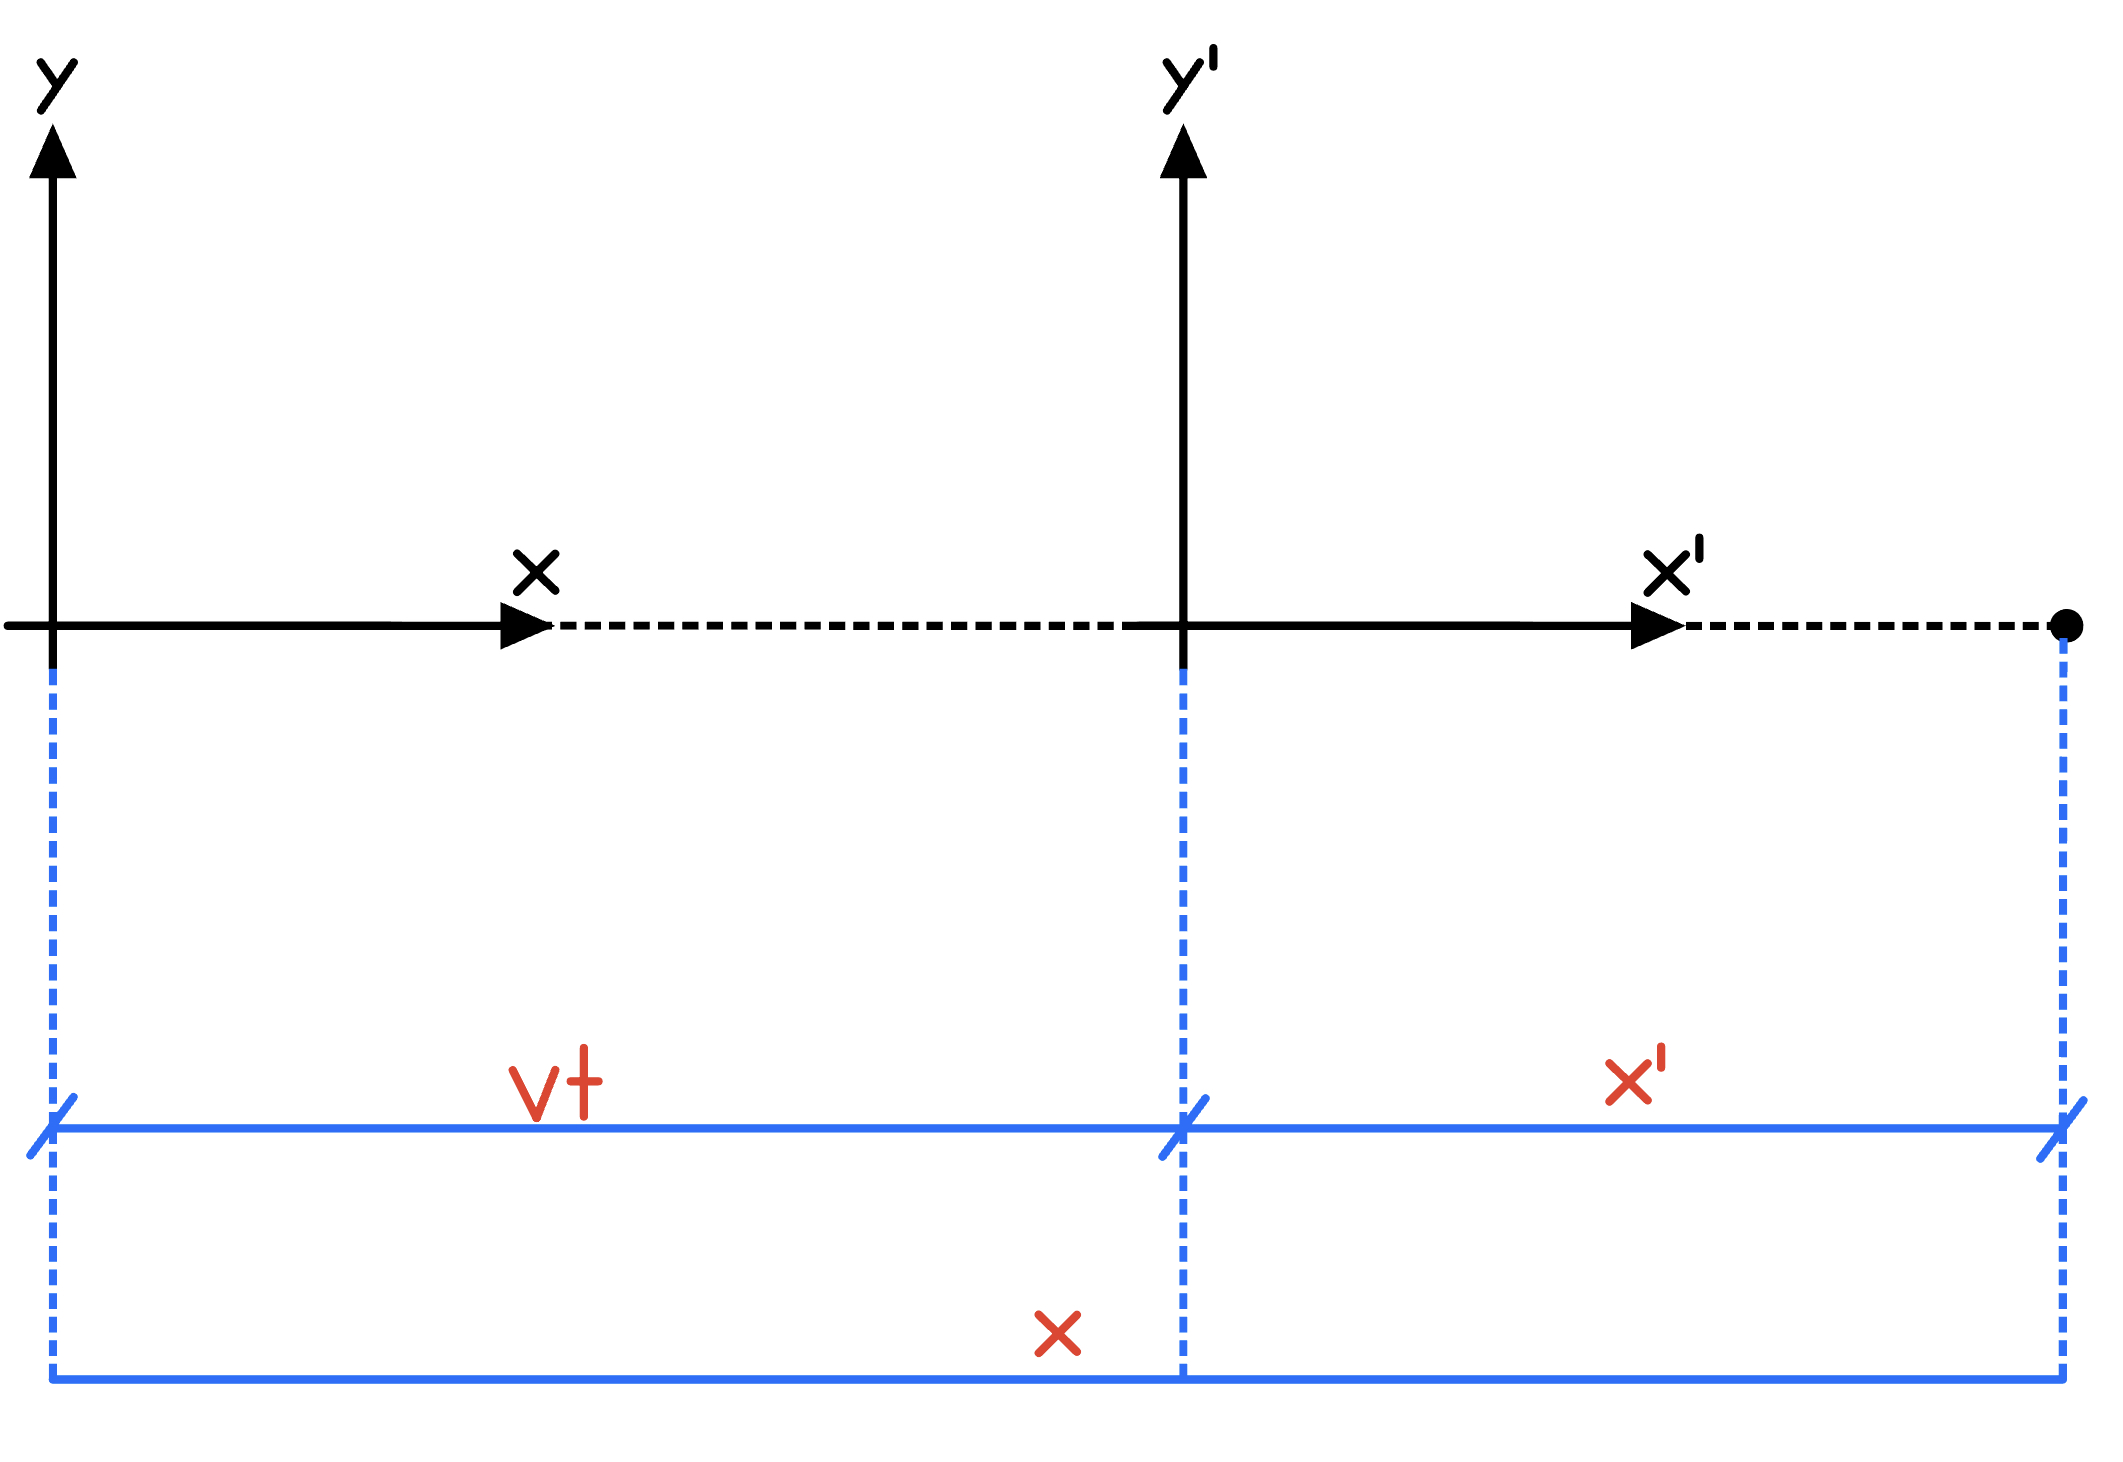
\includegraphics[scale=0.1]{IMG_1140.jpg}}
\end{figure}
Lasst uns annehmen, dass unser Ereignis E von beiden Systemen S und S' wahrgenommen werden kann. Somit hat das Ereignis E in S die Koordinaten $(x,0)$ und die Zeit Koordinate $t$. Unter der Annahme, dass unser Ereignis E in S' im Abstand von x' zu observieren ist, erhalten wir die Koordinaten $(x',0)$. Durch einfache Überlegung erhalten wir, dass der Abstand zwischen den zwei Koordinaten-Systemen $vt$ sein muss (da $s = vt$), angenommen dass sich die Geschwindigkeit $v$ nicht geändert hat. Somit erhalten wir die Gleichungen
\begin{equation} \label{gt1}
    x' = x - vt \tag{gt.1}
\end{equation}
\begin{equation}\label{gt2}
    x = vt + x' \tag{gt.2}
\end{equation}
und da wir dieselben Koordinaten für y und z haben gilt $y' = y, z' = z$. Wenn wir nun nicht mit komplexen Argumenten argumentieren wollen, wieso $t' = t$ ist, können wir theoretisch einfach annehmen, da wir uns linear auf der x-Achse bewegen und annehmen, dass die Verzerrung keinen Effekt auf die y-Achse hat, welches auch zu bedeuten hat, dass sich $t$ nicht verändert.

Zusammengefasst können wir folgende Gleichungen aufstellen:

\begin{equation} \label{gt3}
    x' = x - vt \tag{gt.3}
\end{equation}
\begin{equation}\label{gt4}
    y' = y \tag{gt.4}
\end{equation}
\begin{equation}\label{gt5}
    z' = z \tag{gt.5}
\end{equation}
\begin{equation}\label{gt6}
    t' = t \tag{gt.6}
\end{equation}

\subsubsection{Anwendung der Gleichungen aus 2.2}
Mit diesen Gleichungen \ref{gt3}-\ref{gt6} lässt sich wie schon erwähnt eine Messung in einem Intertialsystem mit der in einem anderen vergleichen. Lasst uns bspw. annehmen, dass wir die Geschwindigkeit eines Motorrads, welches sich in x-Richtung im Inertialsystem S bewegt, nun im Inertialsystem S' messen möchten. Dazu verwenden wir die übliche Beziehung für die Geschwindigkeit $v$, namentlich Weg pro Zeit $v = \dfrac{s}{t}$. Daraus folgt dass man in einem s-t Diagramm die Geschwindigkeit gleich setzen kann mit der Steigung und man somit mittels der ersten Ableitung nach der Zeit von der Strecke $s$ die Geschwindigkeit erhält: $v = \dfrac{d}{dt}(s)$.
Nun auf unsere Situation angewandt erhält man:
\begin{equation*}
    v'_{x} = \dfrac{dx'}{dt'} = \dfrac{d}{dt}(x - vt) = v_{x} - v
\end{equation*}
Nun können wir auch mittels derselben Methode überprüfen, ob alle physikalischen Gesetze in allen Systemen erhalten bleiben. Dies kann man mit mathematischen sowohl als auch empirischen Methoden überprüfen. Mathematisch können wir dies nun mit der Transformation von unseren Gleichungen aus einem System in eines sich mit $v$ zu S konstant bewegenden Inertialsystems S' überprüfen. 

Angenommen wir wollen nun eine klassische Gleichung der Physik, namentlich Newtons zweites Gesetz, in ein anderes System transformieren, um zu verifizieren, dass sich die Beziehung bzw. das Gesetz bei deren Transformation ins neue Inertialsystem sich nicht ändert (es sei gegeben, dass die Tatsache dass jenes Gesetz in allen Inertialsystemen dasselbe ist, experimentell überprüft wurde). Dies können wir nun mit unseren neuen
Galilei-Transformationen verifizieren. Namentlich wie folgt:

Man nehme an, dass der Beobachter in S' sich mit der Geschwindigkeit $v$ relativ zu S in x-Richtung bewegt

\begin{align*}
    F_a' &= m' \cdot a' = m' \dfrac{d^2 x'}{dt'^2} \\
    &= m' \dfrac{d}{dt'}(\dfrac{dx'}{dt'})
\end{align*}
Wir erinnern uns aus der zuvor hergeleiteten Transformation der x-Koordinate von $S \longmapsto S'$; $x' = x - vt$. 
Somit erhalten wir
\begin{equation*}
    F_a' = m\dfrac{d}{dt}(\dfrac{d}{dt}(x - vt)) 
\end{equation*}
Aus $\dfrac{d}{dt}(x - vt) = v_x - v$ angenommen das $v$ eine Konstante ist, ergibt sich
\begin{align*}
    m\dfrac{dv_x}{dt} = ma = F_a
\end{align*}
Aus dem Beweis ist nun ersichtlich, dass die physikalischen Gesetze in der Tat in allen Inertialsystemen erhalten bleiben.

Die Erhaltung der meisten physikalischen Gesetze lässt sich mittels galileischen Transformationen beweisen.
\cite{GT2}

\subsubsection{Matrixform der Galilei Transformation}
Um sich die Berechnungen der Galilei Transformation zu erleichtern kann man deren Matrixschreibweise einführen. Aus grundlegendem Wissen der Linearen Algebra lässt sich folgende Gleichung für die Koordinatenvektoren in verschiedenen Systemen aufstellen. Da wir wissen, dass $x' = x - vt$ entsprechen muss und $t' = t$ ist. Können wir nun eine beliebige Matrix aufstellen, welche durch Matrix-Multiplikation mit den $alten$ Koordinaten die zuvor berechneten neuen Koordinaten im $neuen$ Inertialsystem liefert. Kommen wir nun zur Herleitung dieser beliebigen Matrix.

\begin{equation*}
\begin{pmatrix}
t^{'} \\
x'
\end{pmatrix}=\begin{pmatrix}
a & b \\
c & d
\end{pmatrix}\begin{pmatrix}
t \\
x
\end{pmatrix}=\begin{pmatrix}
t \\
x-vt
\end{pmatrix}
\end{equation*}
Durch Regeln der Matrix-Multiplikation erhalten wir folgende Gleichungen welche es nach den Parametern, $a,b,c$ und $d$ zu lösen gilt.
\begin{align*}
a\cdot t+b \cdot x&=t \\
c\cdot t+d \cdot x&=x-vt
\end{align*}
Lösen wir nun die erste Gleichung nach ihren Unbekannten $a$ und $b$ auf, erhalten wir $a = 1$ und $b = 0$. Wiederholen wir dasselbe Spiel für die zweite Gleichung erhalten wir $c = -v$ und $d = 1 \implies$ 
$ G_T =
\begin{pmatrix}
1 & 0 \\
-v & 1
\end{pmatrix}
$

Bewiesen durch

\begin{equation}
\begin{pmatrix}
t' \\
x'
\end{pmatrix}=\begin{pmatrix}
1 & 0 \\
-v & 1
\end{pmatrix}\begin{pmatrix}
t \\
x
\end{pmatrix}=\begin{pmatrix}
t \\
x-vt
\end{pmatrix}
\end{equation}
Und somit gilt $G_T$ als bewiesen. 

\section{Grundlegendes der speziellen Relativitätstheorie}
\subsection{Mathematische Grundlagen der speziellen Relativitätstheorie}
Zur Lösungen und dem Verständnis der in diesem Kapitel folgenden Phänomene sind einige mathematische Grundkenntnisse nötig. 
In der speziellen Relativitätstheorie und speziell in dieser Arbeit sind vor allem linear algebraische Kenntnisse notwendig und selbstverständlich Analysis an einigen Stellen. Da das Programm aber vor allem auf Kenntnissen der linearen Algebra beruht, werden in diesem Kapitel nur die Grundkenntnisse, welche nötig sind um ein ähnliches Programm zu erstellen, behandelt.

\subsubsection{Vektoren}
Vektoren sollten den Lesern dieser Arbeit zwar bereits bekannt sein, aber falls dies nicht der Fall sein sollte ist hier noch mal eine kurze Erklärung der Grundlagen. In der Mathematik ist ein Vektor eine Größe, die eine Richtung und eine Magnitude (Größe) hat. Vektoren können in verschiedenen Bereichen der Mathematik verwendet werden, zum Beispiel in der Geometrie, der linearen Algebra und der Analysis.
In der Geometrie kann man sich einen Vektor als Pfeil vorstellen, der von einem Anfangspunkt zu einem Endpunkt zeigt. Die Länge des Pfeils entspricht der Magnitude des Vektors, während die Richtung, in die der Pfeil zeigt, die Richtung des Vektors angibt.
In der Linearen Algebra werden Vektoren häufig verwendet, um geometrische Objekte zu beschreiben und zu analysieren. Sie können auch verwendet werden, um Gleichungen zu lösen und Transformationen durchzuführen. In der Analysis werden Vektoren oft verwendet, um Funktionen und ihre Ableitungen zu beschreiben und zu analysieren. \cite{Vektor} Sie können auch verwendet werden, um Integrale zu berechnen und Differentialgleichungen zu lösen. Wir möchten uns im Rahmen dieser Arbeit eher auf den linear algebraischen Aspekt von Vektoren konzentrieren. Nun kurz einige Eigenschaften und Rechenmethoden von Vektoren.

\paragraph{Bestimmung eines Vektors}
Ein Vektor oder besser gesagt ein euklidischer Vektor in $\mathbb{R^3}$ kann folgendermassen dargestellt werden.

\begin{center}
$\Vec{v} = \begin{pmatrix} v_1 \\ v_2 \\ v_3 \end{pmatrix}$
\end{center}

Dabei ist die erste Komponente die X-Richtung, die zweite die Y-Richtung und die dritte die Z-Richtung.
Lasst uns nun bspw. den Vektor $\vv{AB}$ zwischen den beiden Punkten $\color{blue}A = (1,1,1)$ und $\color{red} B = (2,2,2)$ bestimmen.

\begin{center}
$\vv{AB} = \begin{pmatrix} \color{red}2 \color{black}- \color{blue}1 \\ \color{red}2 \color{black}- \color{blue}1 \\ \color{red}2 \color{black}- \color{blue}1\end{pmatrix} = \begin{pmatrix} 1 \\ 1 \\ 1 \end{pmatrix}$
\end{center}

Durch diese Bestimmung des Vektors $\vv{AB}$ lässt sich der folgende Vektor, namens Ortsvektor definieren. Ein Ortsvektor wird definiert als der Vektor zwischen einem Punkt und dem Ursprung des Koordinatensystems.
Bspw.
\begin{align*}
        O &= \begin{pmatrix} 0 \\ 0 \\ 0 \end{pmatrix} \\
        P &= \begin{pmatrix} 1 \\ 1 \\ 1 \end{pmatrix} \\
    \vv{r_P} = \vv{OP} &= \begin{pmatrix} 1 - 0 \\ 1 - 0 \\ 1 - 0  \end{pmatrix} = \begin{pmatrix} 1 \\ 1 \\ 1 \end{pmatrix}
\end{align*}
\cite{Vektor}
\paragraph{Skalare Multiplikation}
\begin{equation*}
    \mu \cdot \begin{pmatrix} x_1 \\ x_2 \\ x_3\end{pmatrix} = \begin{pmatrix} \mu x_1 \\ \mu x_2 \\ \mu x_3\end{pmatrix}
\end{equation*}
\cite{Vektor}\cite{Skalarprodukt}
\paragraph{Skalarprodukt}
\begin{center}
    
    
        $\Vec{p} \cdot \Vec{q} = {\begin{pmatrix} p_1 \\ p_2 \\ p_3 \end{pmatrix} \cdot \begin{pmatrix} q_1 \\ q_2 \\ q_3 \end{pmatrix}} = p_1 q_1 + p_2 q_2 + p_3 q_3 $
\end{center}   
    

\cite{Vektor}\cite{Skalarprodukt}
\paragraph{Kreuzprodukt}
\begin{center}
    
        $\Vec{p} \times \Vec{q} = \begin{pmatrix} p_1 \\ p_2 \\ p_3 \end{pmatrix} \times \begin{pmatrix} q_1 \\ q_2 \\ q_3 \end{pmatrix} = \begin{pmatrix} p_2 q_3 - p_3 q_2\\ p_3 q_1 - p_1 q_3 \\ p_1 q_2 - p_2 q_1 \end{pmatrix}$
    
\end{center}
\paragraph{Norm}
Die Norm eines Vektors ist eine Messgröße für die Größe oder Länge des Vektors. Es gibt verschiedene Definitionen für die Norm eines Vektors, die je nach Kontext verwendet werden können. Die häufigsten Definitionen sind:
\begin{itemize}
    \item Die Euklidische Norm (auch als Längen- oder L2-Norm bezeichnet) eines Vektors v mit n Komponenten wird wie folgt berechnet:
    $||v||_2 = \sqrt{v_1^2 + v_2^2 + \dots + v_n^2}$
    \item Die Manhattan-Norm (auch als L1-Norm oder Taxifahrer-Norm bezeichnet) eines Vektors v mit n Komponenten wird wie folgt berechnet:
    $||v||_1 = |v_1| + |v_2| + \dots + |v_n|$
    \item Die Maximalnorm (auch als L-infinity-Norm oder Maximum-Norm bezeichnet) eines Vektors v mit n Komponenten wird wie folgt berechnet:
    $||v||_\infty = \max(|v_1|, |v_2|, \dots, |v_n|)$
\end{itemize}

Die häufigste Norm und auch die Norm, welche in späteren Berechnungen in dieser Arbeit verwendet wird, ist die Euklidische Norm.


\subsubsection{Matrizen}
Eine Matrix ist ein rechteckiges Array von Zahlen, Symbolen oder Funktionen, die in Reihen und Spalten angeordnet sind. Matrizen werden in der Mathematik und in vielen Anwendungsbereichen, wie der Physik, der Informatik und der Statistik, verwendet. \cite{Elementary Linear Algebra} Um das Ganze einfach zu halten wird in diesem Abschnitt nur kurz gezeigt wie eine Matrix aussieht und was für Operationen man mit ihr durchführen kann und was für Eigenschaften sie sonst noch hat.

Als Beispiel einer Matrix können wir folgende Tabelle in eine Matrix umwandeln.

\begin{tabularx}{0.8\textwidth} { 
  | >{\raggedright\arraybackslash}X 
  | >{\centering\arraybackslash}X 
  | >{\raggedleft\arraybackslash}X | }
 \hline
 1 & 12 & 13 \\
 \hline
 21  & 22  & 23  \\
\hline
\end{tabularx}

Diese Tabelle lässt sich als die folgende Matrix schreiben

$$
\begin{bmatrix}
1 & 12 & 13 \\
21 & 22 & 23 
\end{bmatrix}
$$
Wenn wir dies nun etwas genereller beschreiben möchten dann sieht eine Matrix folgendermassen aus.

$$
\begin{bmatrix}
    a_{11} & a_{12} & \cdots & a_{1n} \\
    a_{21} & a_{22} & \cdots & a_{2n} \\
    \vdots & \vdots &  & \vdots \\
    a_{m1} & a_{m2} & \cdots & a_{mn} 
    
\end{bmatrix}
$$
\cite{Elementary Linear Algebra}

Wenn wir die Matrix nun in kompakter Schreibweise notieren möchten, dann können wir dies folgendermassen tun. $i$ stellt dabei die Reihe und $j$ die Spalte dar.
\begin{equation*}
    [a_ij]
\end{equation*}

\paragraph{Subtraktion,Addition und Multiplikation}
Die wichtigsten Operationen welche man mit Matrizen durchführen kann, sind die folgenden. Addition, Subtraktion und Multiplikation.
Addition ist die simpelste Operation, welche man mit einer Matrix durchführen kann. Wenn wir uns an die Vektor-Addition erinnern, kommen wir schnell darauf, dass Matrizen in derselben Weise operieren. Wenn man eine Matrix $A_{2\times2}$ also eine $2\times2$ Matrix nimmt und diese mit einer weiteren $2\times2$ Matrix $B_{2\times2}$ addiert, dann erhält man folgende Matrix als generelle Lösung für $2\times2$ Matrizen. \cite{Elementary Linear Algebra}

$$
 A + B =
\begin{bmatrix}
    a_{11} + b_{11} & a_{12} + b_{12} & \cdots & a_{1n} + b_{1n} \\
    a_{21} + b_{21} & a_{22} + b_{22} & \cdots & a_{2n} + b_{2n} \\
    \vdots & \vdots &  & \vdots \\
    a_{m1} + b_{m1} & a_{m2} + b_{m2} & \cdots & a_{mn} + b_{mn} 
\end{bmatrix}
$$
Wenn man nun dasselbe für die Subtraktion macht, dann erhält man die folgende Matrix als Lösung für die Subtraktion der Matrix $B$ von $A$. Dabei ist wichtig anzumerken, dass die Lösungen nur gelten, wenn beide Matrizen dieselbe Grösse haben.
$$
 A - B =
\begin{bmatrix}
    a_{11} - b_{11} & a_{12} - b_{12} & \cdots & a_{1n} - b_{1n} \\
    a_{21} - b_{21} & a_{22} - b_{22} & \cdots & a_{2n} - b_{2n} \\
    \vdots & \vdots &  & \vdots \\
    a_{m1} - b_{m1} & a_{m2} - b_{m2} & \cdots & a_{mn} - b_{mn} 
\end{bmatrix}
$$
Um zwei Matrizen zu multiplizieren, müssen sie kompatibel sein, das bedeutet, dass die Anzahl der Spalten in der ersten Matrix der Anzahl der Zeilen in der zweiten Matrix entsprechen muss. Wenn die erste Matrix A m Zeilen und n Spalten hat, und die zweite Matrix B hat p Zeilen und q Spalten hat, dann ist die Matrixmultiplikation $A \cdot B$ definiert, wenn und nur wenn n = p.\cite{Elementary Linear Algebra}

Die Elemente der Ergebnismatrix C werden berechnet indem man jedes Element der i-ten Zeile und jeder Spalte der j-ten Spalte der ersten Matrix mit dem entsprechenden Element der zweiten Matrix multipliziert und die Produkte summiert:

$$C_{i,j} = \sum_{k=1}^{n} A_{i,k} \cdot B_{k,j}$$

Wenn wir diese Formel nun ausführlich anhand einer Matrix sehen möchten erhalten wir folgendes Beispiel
$$
 \begin{bmatrix}
     a_{11} & a_{12} & \cdots & a_{1n}\\
     a_{21} & a_{22} & \cdots & a_{2n}\\ 
     \vdots & \vdots & \ddots & \vdots\\ 
     a_{m1} & a_{m2} & \cdots & a_{mn} 
 \end{bmatrix}
 \times
 \begin{bmatrix}
     b_{11} & b_{12} & \cdots & b_{1p}\\
     b_{21} & b_{22} & \cdots & b_{2p}\\ 
     \vdots & \vdots & \ddots & \vdots\\ 
     b_{n1} & b_{n2} & \cdots & b_{np} 
 \end{bmatrix}
  =
 \begin{bmatrix}
     c_{11} & c_{12} & \cdots & c_{1p}\\
     c_{21} & c_{22} & \cdots & c_{2p}\\ 
     \vdots & \vdots & \ddots & \vdots\\ 
     c_{m1} & c_{m2} & \cdots & c_{mp} 
 \end{bmatrix}
$$
$$ c_{ij}= a_{i1} b_{1j} + a_{i2} b_{2j} +\cdots+ a_{in} + b_{nj} = \sum_{k=1}^n a_{ik}b_{kj} $$ 

\paragraph{Determinante}
Eine weitere wichtige Operation die mit Matrizen durchgeführt werden kann, ist die Bestimmung der Determinante. Diese wird bei der Herleitung der Lorentz-Transformation in einem späteren Kapitel angewandt.

Eine Determinante ist ein Skalar, der aus einer Matrix berechnet wird und bestimmte Eigenschaften der Matrix beschreibt. Sie wird auch als "Determinant" bezeichnet. Die Determinante einer Matrix wird häufig in der Linearen Algebra verwendet, um die Invertierbarkeit einer Matrix zu bestimmen und um Lösungen für Gleichungssysteme zu finden.\cite{Elementary Linear Algebra}

Die Determinante einer Matrix A, die als det(A) oder $\left|A\right|$ bezeichnet wird, wird wie folgt berechnet:

Für eine 2x2 Matrix A hat sie die Form:

\begin{equation*}
\left|A\right| = a \cdot d - b \cdot c
\end{equation*}

Für eine 3x3 Matrix A hat sie die Form:

\begin{equation*}
\left|A\right| = a \cdot (e \cdot i - f \cdot h) - b \cdot (d \cdot i - f \cdot g) + c \cdot (d \cdot h - e \cdot g)
\end{equation*}
Für eine nxn Matrix A hat sie die Form:

\begin{equation*}
\left|A\right| = a_1 \cdot \left|A_1\right| - a_2 \cdot \left|A_2\right| + a_3 \cdot \left|A_3\right| - ... - a_n \cdot \left|A_n\right|
\end{equation*}

Wobei $a_1$ bis $a_n$ die Elemente der ersten Zeile von A sind und $A_1$ bis $A_n$ die Minoren von A sind (die Determinanten der Matrix, die entstehen, wenn man die erste Zeile und Spalte von A entfernt).
Die Leibniz-Formel ist eine Möglichkeit, die Determinante einer nxn Matrix zu berechnen. Sie besagt, dass die Determinante einer Matrix A gleich der Summe der Produkte der Elemente auf der Hauptdiagonalen ist, die jeweils von der Anzahl der möglichen Permutationen ihrer Indizes abgezogen werden:

$$\left|A\right| = \sum_{k=1}^n (-1)^{p_k} a_{1,k} M_{1,k}$$

Wobei $p_k$ die Anzahl der Vertauschungen von Indizes ist, die benötigt werden, um k auf die Hauptdiagonale zu bringen, und $M_{1,k}$ die Determinante der Matrix ist, die entsteht, wenn man die erste Zeile und Spalte von A entfernt und die Elemente auf der Hauptdiagonalen ersetzt.

Hier ist ein Beispiel für die Berechnung der Determinante einer 3x3 Matrix A mit Hilfe der Leibniz-Formel:

\begin{align*}
\left|A\right| &= a_{1,1} M_{1,1} - a_{1,2} M_{1,2} + a_{1,3} M_{1,3} \\
&= a_{1,1} \cdot \left|A_1\right| - a_{1,2} \cdot \left|A_2\right| + a_{1,3} \cdot \left|A_3\right|
\end{align*}

Wobei $A_1$, $A_2$ und $A_3$ die Minoren von A sind (die Determinanten der Matrizen, die entstehen, wenn man die erste Zeile und Spalte von A entfernt).
Um die Determinante einer nxn Matrix A mit Hilfe der Leibniz-Formel zu berechnen, muss man diesen Prozess für jedes Element auf der Hauptdiagonalen wiederholen. Die Gesamtdeterminante ist dann die Summe aller dieser Produkte.
\cite{Wikipedia Determinant}

\paragraph{Metrik}
Ein anderes Kozept der Linearen Algebra, welches in der Herleitung der Matrixform der Lorentztransformation verwendet wird, ist die sogenannte Metrik.
Eine Metrik ist eine Funktion, die zwei Elemente einer Menge definiert und ihre Distanz zueinander angibt. Sie muss bestimmte Eigenschaften erfüllen, um als Metrik zu gelten:

\begin{itemize}
    \item Distanznull: $d(x,x) = 0$ für alle $x$ in der Menge
    \item Symmetrie: $d(x,y) = d(y,x)$ für alle $x,y$ in der Menge
    \item Triangleungleichung: $d(x,y) + d(y,z) \geq d(x,z)$ für alle $x,y,z$
\end{itemize}

Ein Beispiel für eine Metrik ist die euklidische Distanz in der Euklidischen Ebene. Sie wird wie folgt berechnet \cite{Metrik ED}:

\begin{align*}
d(x,y) &= \sqrt{(x_1 - y_1)^2 + (x_2 - y_2)^2} \\
d(x,y) &= \sqrt{(x_1 - y_1)^2 + (x_2 - y_2)^2} = \sqrt{(x_1^2 - 2x_1y_1 + y_1^2) + (x_2^2 - 2x_2y_2 + y_2^2)} \\
&= \sqrt{x_1^2 - 2x_1y_1 + y_1^2 + x_2^2 - 2x_2y_2 + y_2^2}\\
&= \sqrt{(x_1^2 + x_2^2) - 2(x_1y_1 + x_2y_2) + (y_1^2 + y_2^2)}\\
&= \sqrt{(x_1^2 + x_2^2) - 2 \cdot \left( \begin{pmatrix} x_1 \ x_2 \end{pmatrix} \cdot \begin{pmatrix} y_1 \ y_2 \end{pmatrix} \right) + (y_1^2 + y_2^2)}
\end{align*}
\cite{LA}
\paragraph{Transponieren einer Matrix}
Die Transponierung einer Matrix ist der Vorgang, bei dem die Zeilen und Spalten einer Matrix vertauscht werden. Die transponierte Matrix wird als $A^T$ bezeichnet.

Hier ist eine Matrix A:
\begin{equation*}
A = \begin{pmatrix}
a_{1,1} & a_{1,2} & a_{1,3} \\\
a_{2,1} & a_{2,2} & a_{2,3} \\
a_{3,1} & a_{3,2} & a_{3,3} \
\end{pmatrix}
\end{equation*}

Die transponierte Matrix $A^T$ hat die Form:

\begin{equation*}
A^T = \begin{pmatrix}
a_{1,1} & a_{2,1} & a_{3,1} \\
a_{1,2} & a_{2,2} & a_{3,2} \\
a_{1,3} & a_{2,3} & a_{3,3} \\
\end{pmatrix}
\end{equation*}

Man kann auch sagen, dass die Elemente $a_ij$ der Matrix A an der Stelle (i, j) in der transponierten Matrix $A^T$ an der Stelle (j, i) stehen.\cite{Elementary Linear Algebra}


\subsection{Was ist die Spezielle Relativitätstheorie?}
Wenn man die Frage kurz beantworten möchte, kann man sagen, dass die spezielle Relativitätstheorie sich mit dem vergleichen zweier Datensätze, welche jeweils dasselbe physikalische Phänomen in einem Bezugssystem behandeln und welche von zwei verschiedenen Beobachtern betrachtetet werden, welche sich relativ zum Bezugssystem des stattfindenden physikalischen Phänomens bewegen. \cite{Univie Spezielle Relativittstheorie}

Das vergleichen der beiden Datensätze führte zu unglaublichen Ergebnissen. Nach der galileischen Physik hat ein Ereignis mit der Zeitspanne $\delta t$ egal von welchem Beobachter aus dieselbe Dauer. Nach dem Michelson-Morley-Experiment kamen jedoch Zweifel an der Richtigkeit dieses Zusammenhangs auf. Das Michelson-Morley-Experiment sollte die Geschwindigkeit der Erde relativ zum Lichtäther \cite{Michelson Morley} auf der Bahn um die Sonne nachweisen. Der sogenannte Lichtäther war ein Medium in welchem sich das Licht gleich wie Schallwellen verhalten sollte. Das Experiment zeigte, dass die "Bewegung gegen den Äther" keinen Einfluss auf die Lichtgeschwindigkeit hatte \cite{Michelson Morley}. Alle physikalischen Theorien, welche sich auf den Äther bezogen hatten, stellten Problematiken dar, welche nur mit der Hilfe der speziellen Relativitätstheorie gelöst werden konnten. \cite{Michelson Morley}

Das Michelson-Morley-Experiment bewies die Invarianz der Lichtgeschwindigkeit egal in welchem Bezugssystem und war somit der Funke, welcher die spezielle Relativitätstheorie als Fundament der modernen Physik antreiben konnte. Diese Invarianz ist unerklärbar durch die galilieische Physik. Wirft man einen Ball aus einem Zug mit einer Geschwindigkeit von 25 km/h und wird von einem Zug überholt, welcher sich mit 50 km/h bewegt, so bewegt sich der Ball relativ zum Boden mit 75 km/h. Gemäss galileischer Physik werden die Geschwindigkeiten der beiden Systeme addiert, wenn sie vom System des Bodens beobachtet werden. Wenn sich nach galileischer Physik alle Teilchen im Universum so verhalten würden, wäre die Tatsache, dass die Lichtgeschwindigkeit in allen Bezugssystem invariant ist, unerklärbar gewesen. \cite{Univie Spezielle Relativittstheorie}

Nach der Veröffentlichung der speziellen Relativitätstheorie durch Albert Einstein wurden Voraussagen bezogen auf die Zeit innerhalb verschiedener Referenzsysteme gemacht, welche wir heute als Zeitdilatation kennen. Jene ist nur möglich, wenn die Zeitspanne bezogen auf zwei Referenzsysteme nicht gleich sein muss. Dies wiederum führte zum sogenannten \emph{Zwillings Paradoxon} und weiteren Paradoxen. Nebst der Tatsache der Verschiebung der Zeit ist der Fakt der Längenkontraktion ein sehr wichtiger. Das soll bedeuten, dass sich die Zeiten, sowie die Längen der beobachteten physikalischen Phänomene, welche von verschiedenen Beobachtungssystemen angeschaut werden, nicht gleichen müssen und sogar total verschiedene Resultate erhalten, welche sich jedoch nach newtonischer Mechanik erklären lassen. Dabei ist wichtig anzumerken, dass alle physikalischen Gesetze in allen Bezugssystemen dieselben sind.
\cite{Univie Spezielle Relativittstheorie}
\cite{University Physics}

Dies führt uns nun zu einer der wichtigsten Folgen der speziellen Relativitätstheorie. Die Zeit ist nun nicht mehr eine invariante Grösse, sie verändert sich genau wie die Koordinaten eines Punktes, betrachtet aus verschiedenen Perspektiven. Die Distanzen im Raum sind nun auch nicht mehr dieselben, wenn sich Objekte relativ zu einem Beobachter bewegen. Die spezielle Relativitätstheorie weist nun also eine neue Koordinate eines herkömmlichen Vektors hin, welche abhängig von Raum und Zeit zu sein scheint. So einen Vektor nennt man Minkowski-Vektor oder 4-er Vektor, nach Minkowski-Raum-Zeit-Diagramm. \cite{Univie Spezielle Relativittstheorie} \cite{Principles of Physics}
Aus letzterem Konzept ergibt sich die Einführung eines neuen Begriffs, namentlich Interitalsystem. Ein Inertialsystem ist ein Bezugssystem in dem sich eine Masse gleichförmig fort bewegt oder ein kräftefreier Körper stillsteht. \cite{Inertialsystem} Aufgrund der Postulierung, dass Massen sich in Inertialsystemen gleichförmig bewegen, lässt sich schliessen, dass alle Bezugsysteme, welche sich geradlinig-gleichförmig gegenüber einem Inertialsystem bewegen, ebenfalls Inertialsysteme sind. 

Es lässt sich sagen, dass die Erschaffung dieser neuen Konzepte zu drastischen Revisionen des bisherig Erlernten führte. Es mussten bspw. relativistische Versionen von Konzepten entworfen werden, um die Realität nach Einstein besser erklären zu können. Es entstanden auch neue Konzepte auf alten Grundlagen. Bspw. der relativistische Doppler-Effekt, welcher sich nur durch die Relativität erklären lässt, sich aber aus dem Konzept von Christian Doppler ergeben hat. 

Ich möchte nun eine wichtige Anmerkung machen: Es wird oftmals gesagt, dass sich die spezielle Relativitätstheorie nur mit dem Zusammenhang der geradlinig-gleichförmigen Bewegung auseinandersetzt und dass der Zusammenhang der beschleunigten Bewegung in der Allgemeinen Relativitätstheorie geklärt wird. Dies ist jedoch eine grundlegend falsche Annahme, denn die spezielle Relativitätstheorie beschäftigt sich mit der Beschreibung und Analyse physikalischer Phänomene und somit auch Phänomene der beschleunigten Bewegung. Jedoch nur solange jene in einem Inertialsystem beobachtet und in Bezug auf dieses beschrieben werden. \cite{Univie Spezielle Relativittstheorie} Die allgemeine Relativitätstheorie bezieht sich hingegen auf die Annahme, dass es gar keine Inertialsysteme gibt. 

Nach Einstein lassen sich zwei sogenannte Postulate aufstellen. Postulate sind Formulierungen und Annahmen ohne welche sich die darauf aufbauende Theorie nicht erklären lässt. Dabei ist wichtig anzumerken, dass theoretisch auch andere Überlegungen möglich sind und nicht ausgeschlossen werden können. Die sogenannten Postulate können aus Experimenten geschlossen oder aus philosopischen Überlegungen erkannt werden, müssen sich jedoch durch experimentelle Verfahren beweisen lassen.

\subsubsection{Einsteins Postulate}
Einsteins \textbf{Erstes} Postulat, dass sogenante Prinzip der Relativität, besagt, dass alle physikalischen Gesetze in allen Inertialsystemen gleich sind. Wenn sie nicht gleich wären, dann könnte die Richtigkeit eines Inertialsystems angezweifelt werden und es würde somit nur \emph{ein richtiges Ergebnis} geben. Ein gutes Beispiel zur Verdeutlichung dieser Tatsache ist:
Man nehme an zwei Kinder würden auf einem Zug mit einem Ball spielen und wir würden uns auf einem Zug mit konstanter Geschwindigkeit bewegen. Egal was man tut, man kann aus den Beobachtungen nicht schliessen, ob oder wie schnell sich der Zug bewegt. Dass liegt genau daran, dass alle physikalischen Gesetze in allen Inertialsystemen dieselben sind. \cite{University Physics} Kurzgesagt sind andere physikalischen Phänomene, wie die von Faraday oder des Elektromagnetismus in allen Ergebnissen gleich und man erhält die gleichen Resultate. Dabei ist das wichtigste Phänomen, die Voraussage der elektromagnetischen Strahlung, welche sich aus Maxwells Gleichungen ergeben. Nach diesem Phänomen bewegen sich Licht und andere elektromagnetische Wellen in einem Vakuum mit derselben konstanten Geschwindigkeit, namentlich $299'792'458 m/s$. 
\cite{University Physics}
Aus letzterem entsteht Einsteins \textbf{Zweites} Postulat. Wie bereits in einem vorherigen Abschnitt erklärt, nahmen die Physiker im 19. Jahrhundert an, dass sich Licht, durch ein sogenanntes Medium, namens Äther, wie Schallwellen durch die Luft bewegen. Das wie schon erwähnte Michelson-Morley-Experiment war bei der Auflösung der Ätherphysik zentral und führte wie schon gesagt zu Einsteins Überlegungen. Einsteins weltverändernde Überlegung bestand in der Tatsache und des empirischen Beweises seiner Vermutungen des ersten Postulats, welches zum Schluss kam, dass Maxwell's Gesetze in allen Inertialsystemen gleich sind und dass somit die Lichtigeschwindigkeit in allen Inertialsystemen dieselbe sein muss. Jenes wurde wie schon erwähnt durch das Michelson-Morley-Experiment bewiesen. Somit lautet Einsteins zweites Postulat, dass die Lichtgeschwindigkeit im Vakuum in allen Inertialsystemen dieselbe ist und unabhängig von der Bewegung der Quelle ist. \cite{University Physics} Es lässt sich folgendes Gedankenexperiment als Beweis dieses Phänomens aufstellen. Man nehme an das zwei Beobachter die Lichtgeschwindigkeit in einem Vakuum messen, bspw. im Weltall. Ein Beobachter bewegt sich gleichförmig-gradlinig relativ zur Lichtquelle und ein anderer bleibt still. Nach dem Prinzip der Relativität, welche besondere Bezugssysteme, dir wir als Inertialsysteme bezeichnet haben, annimmt, müssen beide Beobachter dasselbe Resultat für die Lichtgeschwindigkeit erhalten.
\cite{University Physics}

\newpage

\subsection{Grundlegende Phänomene}
Ich möchte nun auf grundlegende Ideen verweisen, welche zentral für die spezielle Relativitätstheorie sind.

\subsubsection{4er-Vektoren}
Die bereits erwähnten \textbf{4er-Vektor}en oder auch Minkowski-Vektoren, welche durch drei Raum- und eine Zeitkoordinate definiert werden. Die grundlegende Idee entspricht hierbei die Analyse und das Verstehen verschiedener Datenpunkte betrachtet aus den Perspektiven zwei verschiedener Beobachter, welche sich gleichförmig zueinander bewegen und somit Inertialsysteme bilden. \cite{Principles of Physics}

Ein Vierervektor, ein Derivat der Relativitätstheorie, ist ein Vektor im reellen, vierdimensionalen Raum mit indefiniten Längenquadrat. Dies bedeutet, dass dieses Längenquadrat auch invariant unter den Lorentz-Transformationen ist, sowie dies eines $R^3$ Vektors. Diese Invarianz bedeutet, dass das Längenquadrat in allen Inertialsystemen gleich ist. In unserem Fall der speziellen Relativitätstheorie nehmen wir an, dass die Komponenten des Vierervektors Zeit- sowie Ortskoordinaten eines Ereignisses beinhalten, als auch die Energie die Energie und den Puls eines Teilchens.

In zwei sich unterschiedliche bewegenden Inertialsystem lassen sich die Komponenten der Vierevektoren von einem Inertialsystem ins Nächste mittels des Lorentz-Boosts übertragen.
Man verwendet ${a^\mu = (a^0, a^1, a^2, a^3)}$ als Notation für einen \textbf{kontravarianten 4-er Vektor} und  ${a_\mu = (a_0, a_1, a_2, a_3)}$ für einen \textbf{kovarienten 4-er Vektor}.

Der Ortsvektor wird definiert durch eine Zeitkomponente {t} und Raumkoordinaten $ \overrightarrow x = (x, y, z)$. Die Zeitkoordinate wird mit der Lichtgeschwindigkeit $c$ multipliziert, so dass sie wie die Raumkoordinaten die Dimension einer Länge hat. 

\paragraph{Kontravriant und Kovariant}
Die kovariante Darstellung des Orts-Vierervektors in der speziellen Relativitätstheorie entspricht
\begin{equation*}
x_\mu = (ct, x, y, z) = (ct, x)
\end{equation*}
und die kontravariante Darstellung entspricht
\begin{equation*}
    x^\mu = \begin{pmatrix}
        ct \\ x \\ y \\ z
    \end{pmatrix}
\end{equation*}
\paragraph{Längenquadrat} 
Das invariante Längenquadrat $ds^2$ entspricht dem Skalarprodukt des kontravarianten und des kovarianten Vierervektors
\begin{equation*}
    ds^2 = dx_\mu \cdot dx^\mu = (dx^0)^2 - (dx^1)^2 - (dx^3)^2
\end{equation*}
Aus dem 4er-Vektor der speziellen Relativitätstheorie ergibt sich das folgende Längenquadrat
\begin{align*}
    ds^2 &= dx_\mu \cdot dx^\mu = c^2 dt^2 - dx^2 - dy^2 - dz^2 \\
    s^2 &= (c^2 t^2 - x^2 - y^2 - z^2) = (c^2 {t'}^2 - {x'}^2 - {y'}^2 - {z'}^2)
\end{align*}

\newpage
\paragraph{Vierergeschwindigkeit}
Der Begriff der Vierergeschwindigkeit ist ebenfalls wichtig für die Simulation der bewegten Objekte und die Herleitung der Lorentz-Transformation. Die Vierergeschwindigkeit $\mathbf{v}$ erhält man durch das Differenzieren des Ortsvierervektors $x$ nach der Eigenzeit (mehr zu Eigenzeit in \ref{ZD}) $d\tau$. Die Eigenzeit ist definiert als 

\begin{align*}
    d\tau &= \frac{1}{\gamma} dt \\
    x &= \begin{pmatrix} ct \\ x \\ y \\ z\end{pmatrix} \\
    \mathbf{v} &= \frac{dx}{d\tau} = \gamma \cdot \frac{d}{dt} \begin{pmatrix} ct \\ x \\ y \\ z\end{pmatrix} \\
    &= \gamma \begin{pmatrix} c \\ v_x \\ v_y \\ v_z\end{pmatrix} \\
    \gamma &= \frac{1}{\sqrt{1-\frac{{v_x}^2 + {v_y}^2 + {v_z}^2}{c^2}}}
\end{align*} \cite{4erV}

\subsubsection{Lorentz-Transformation}
\paragraph{Was sind Lorentz-Transformationen}
Nach der Einführung in klassische Transformationen, wie die Galilei Transformation, stellt sich die Frage: Was gilt nun bei grösseren Geschwindigkeiten? Um diese Frage zu beantworten braucht man die Lorentz-Transformationen. Da die Galilei Transformationen gute Näherungen bei irdischen Geschwindigkeiten bieten, lassen sich jene auch mittels einiger Modifikationen in die Lorentz-Transformationen umformen. Wie schon gesagt, die Galilei Transformationen bieten gute Approximationen bei kleinen Geschwindigkeiten dar, sie sind jedoch aber nicht von Nutzen bei höheren Geschwindigkeiten, sowie bei der Elektrodynamik. Ohne die Lorentz-Transformationen könnte man das Verhalten von elektromagnetischen Wellen nicht erklären. Namentlich liessen sich die Maxwellschen Gleichungen und die konstante Lichtgeschwindigkeit (im Vakuum) $c$ durch die Galilei-Transformationen nicht erklären, da in Galilei Transformationen die Lichtgeschwindigkeit relativ zur Bewegung und zu den Referenzpunkten ist. Somit wird sie sich in verschiedenen Richtungen unterscheiden, welches Maxwells Theorie widersprechen würde. Ebenfalls konnte man die Ergebnisse des Michelson-Morley Experiments (Experiment welches die Geschwindigkeit der Erde relativ zum Lichtäther bestimmen sollte)\cite{Michelson Morley} nicht mit den Galileischen Gleichungen erklären. Es mussten also neue Gleichungen her. Diese Gleichungen beinhalteten nun neue Überlegungen, wie dass sie eine neue, vierdimensionale Raumzeit annahmen, welche Zeit- und Raumkoordinaten vereinen sollte. Es gelten auch hier wieder die Erhaltung der physikalischen Gesetze und anders als bei den Galilei Transformationen werden die Abstände im Minkowski-Raum ($\mathbb{R}^4$) eingehalten. Ohne die Lorentz-Transformation wäre die spezielle Relativitätstheorie unvorstellbar und unerklärbar gewesen. Lorentz-Transformationen bilden wie die Galilei Transformationen Gruppen, welchen folgenden Operationen folgen:

\begin{itemize}
    \item Mehrere aufeinanderfolgende Lorentz Transformationen können mit einer Lorentz Transformation beschrieben werden
    \item Eine Lorentz-Transformation von einem Inertialsystem in dasselbe wird ebenfalls als Lorentz-Transformation bezeichnet
    \item Es existiert eine inverse Lorentz-Transformation, welche die Koordinaten wieder ins ursprüngliche Inertialsystem zurück transformiert
    \item Die Determinante der Transformationsmatrix entspricht eins
    
\end{itemize}


\paragraph{Anwendungen der Lorentz-Transformation}
Die Lorentz Transformation lässt sich im Gegensatz zu den Galilei Transformationen unter fast allen Bedingungen einsetzen, namentlich ist sie bei sehr grossen, wie auch sehr kleinen Geschwindigkeiten anwendbar und liefert bei allen akkurate Ergebnisse, welche mit experimentellen Resultaten übereinstimmen. Sie finden vorallem Anwendung in der speziellen Relativitätstheorie in welcher sie als Koordinatentransform und als Grundlage deren Konsequenzen, wie der Zeitdilatation, Längenkontraktion oder der relativistischen Massezunahme, sowie bei Einsteins Zwillings Paradoxon und vielen weiteren Überlegungen. Ebenfalls finden sie Gebrauch in der Simulation von Systemen, namentlich dem Ziel meiner Arbeit, der Simulation von verschiedenen Objekten mittels der Relativitätstheorie. Ohne die Lorentz Transformation wäre meine Simulation undenkbar gewesen und würde somit auch nicht akkurate Resultate liefern. Die Lorentz-Transformation kann in der Simulation namentlich Anwendung finden, indem man sie mehrere Male für verschiedene Punkte (oder auch Funktionen) wiederholt und diese dann grafisch darstellt und somit auch deren Bewegung darstellt. Mit Lorentz-Transformationen kann man also Bewegungen von Teilchen bei ganz grossen und ganz kleinen Geschwindigkeiten simulieren.

\paragraph{Herleitung der Lorentz Transformation}
Herleitung der Lorentz-Transformation aus den Galilei-Transformationen.
Galilei-Transformationen:
\begin{equation}
\label{hlt.1}
    t' = t, x' = x -vt, y' = y, z' = z \tag{hlt.1}
\end{equation}
\begin{center}
\label{Lorentz-Transformations}
\begin{tikzpicture}
   \tkzInit[xmax=2,ymax=2,xmin=-2,ymin=-2]
   \tkzAxeXY
   \draw[ thick,latex-latex] (0,0) -- (2,1) node[anchor=south west] {$x'$}; % two points for drawing 2x+y=2
   \draw[ thick,latex-latex] (0,0) -- (1,2) node[anchor=south west] {$ct'$}; % two points for drawing 2x+y=2
  \tkzText[above](0,4){$v$}
  
\end{tikzpicture}

\qquad

\begin{tikzpicture}
   \tkzInit[xmax=2,ymax=2,xmin=-2,ymin=-2]
   \tkzAxeXY
   \draw[ thick,latex-latex] (0,0) -- (-2,1) node[anchor=south west] {$x$}; % two points for drawing 2x+y=2
   \draw[ thick,latex-latex] (0,0) -- (-1,2) node[anchor=south west] {$ct$}; % two points for drawing 2x+y=2
  \tkzText[above](0,4){$-v$}
  \end{tikzpicture}

\end{center}

Wir nehmen zunächst an, dass sich unsere beiden Koordinatensystem aufeinander zu bewegen.
Durch die Symmetrie der Koordinatenachsen aufgrund der Lichtgeschwindigkeit muss sich ein bestimmter Faktor ergeben, welcher die Längenerhaltung innerhalb zwei Inertialsystem ermöglicht. Dies ist mit den Galilei-Transformationen nicht möglich. Aufgrund dieser Annahme ergeben sich folgende Gleichungen:
\begin{equation}\label{hlt.2}
x' = \gamma (x - vt), x = \gamma (x' + vt')\tag{hlt.2}
\end{equation}
Man multipliziere {x} mit {x'}
\begin{equation} \label{hlt.3}
xx' = \gamma^2 (xx' + xvt' -vtx' - v^2tt') \tag{hlt.3}
\end{equation}
Aufgrund der Tatsache dass ${x = ct}$ und ${x' = ct'}$ ist, erhalten wir nun:
\begin{equation} \label{hlt.4}
ctct' = \gamma^2(ctct' + ctvt' - vtct' -v^2tt')\tag{hlt.4}
\end{equation}
\begin{equation}
\label{hlt.5}
c^2 = \gamma^2(c^2 - v^2) \tag{hlt.5}
\end{equation}
\begin{equation} \label{hlt.6}
\gamma^2 = \frac{c^2}{c^2 - 1} = \frac{1}{1 - \frac{v^2}{c^2}} \tag{hlt.6}
\end{equation}
\begin{equation} \label{hlt.7}
\gamma = \frac{1}{\sqrt{{1 - \frac{v^2}{c^2}}}} \tag{hlt.7}
\end{equation}
Einfacherheitshalber setzen wir $\beta = \frac{v}{c}$. Dies führt zu:
\begin{equation} \label{hlt.8}
\gamma = \frac{1}{\sqrt{{1 - \beta}}} \tag{hlt.8}
\end{equation}

Mittels der Gleichungen \ref{hlt.2} und \ref{hlt.7} lässt sich folgende Beziehung aufstellen, um t' im neuen Inertialsystem zu bestimmen.

\begin{equation} \label{hlt.9}
\frac{x}{\gamma} = x' + vt' \tag{hlt.9}
\end{equation}
\begin{equation}\label{hlt.10}
\frac{x}{\gamma} - x' = vt' \tag{hlt.10}
\end{equation}\begin{equation} \label{hlt.11}
\frac{x}{\gamma v} - \frac{x'}{v} = t' \tag{hlt.11}
\end{equation}

Mit der Beziehung ${x' = \gamma (x - vt)}$, diese gilt da Licht ein Eigenvektor ist und laut Einsteins Postulaten in allen Inertialsystemen gleich sein muss und wenn sich $x$ somit linear bewegt, bewegt sich das Objekt nicht schneller als Lichtgeschwindigkeit, somit lässt sich folgende Gleichung aufstellen
\begin{equation} \label{hlt.12}
t' = \frac{x}{\gamma v} - \frac{\gamma(x - vt)}{v} \tag{hlt.12}
\end{equation}
\begin{equation}\label{hlt.13}
t' = \gamma (\color{red}\frac{x}{\gamma^2 v} - \frac{x}{v} \color{black}+ t) \tag{hlt.13}
\end{equation}
let $z = \color{red}\frac{x}{\gamma^2 v} - \frac{x}{v}$
\begin{align} \label{hlt.14}
z &= \frac{x}{\gamma^2 v} - \frac{x}{v} \notag\\
&= x(\color{violet}\frac{1}{\gamma^2 v} - \frac{\gamma^2}{\gamma^2 v}) \tag{hlt.14}
\end{align}
Nun vereinfachen wir $u = \color{violet}\frac{1}{\gamma^2 v} - \frac{\gamma^2}{\gamma^2 v}$
\begin{equation}\label{hlt.15}
u = \frac{1-\gamma^2}{\gamma^2 v} = \frac{-v}{c^2} \tag{hlt.15}
\end{equation}
Aus \ref{hlt.14} und der Vereinfachung \ref{hlt.15} ergibt sich
\begin{equation} \label{hlt.16}
z = x(u) = x(\frac{-v}{c^2}) \tag{hlt.16}
\end{equation}
Durch einsetzen von \ref{hlt.16} in \ref{hlt.13} erhalten wir
\begin{equation} \label{hlt.17}
t' = \gamma (t - \frac{v}{c^2}x) \tag{hlt.17}
\end{equation}

\newpage
\paragraph{Herleitung des Lorentz-Boost und anderen Matrix-Formen}

Erstmal müssen wir einige Gesetze für Inertialsysteme vereinbaren. Die Inertialsysteme sind nach folgenden Postulaten beschreibbar:
\begin{itemize}
\item a) {$\overrightarrow{\ddot{x}} = 0$}, das Trägheitsgesetz
\item b) Das zweite Postulat besagt, dass alle physikalischen Gesetze in allen Inertialsystem gleich sind.
\end{itemize}
Dazu nehmen wir nochmals an, dass wir ein Inertialsystem haben, in welchem wir folgendes als Koordinaten verwenden.

\begin{equation} \label{lt.0}
x = (x_0, x_1, x_2, x_3) = (ct,\overrightarrow x) \tag{lt.0}
\end{equation}
Das Trägheitsgesetz sagt aus, dass die letzte Gleichung durch eine Gerade darstellbar ist. Dies bedeutet dass die gesuchte Transformationsmatrix eine bijektive Abbildung eines affinen oder projektiven Raumes auf sich selbst darstellt, bei welcher jede Gerade auf eine andere Gerade abgebildet wird und somit geradentreu sind. 
\begin{equation} \label{L1}
x'^\mu = {{A^\mu}_\nu} {x^\nu} + a^\mu \tag{lt.1}
\end{equation}
Jenes ist ist die Schreibweise der Einsteinschen Summenkonvention. Die Summenkonvention von Einstein besagt, dass in einer Summe von Termen (wie zum Beispiel die Summe von Energie-Termen), die über die verschiedenen Zustände eines Systems gehen, nur solche Zustände berücksichtigt werden sollten, die sich von einander unterscheiden. Mathematisch gesehen sagt Einstein eigentlich, dass aufgrund der Eigenschaft des Levi-Cita Symbols $\epsilon_ijk$ wir Terme, welche sozusagen doppelt vorkommen streichen können.
\ref{L1} lässt sich ebenfalls als {$x' = Ax + a$} schreiben. Dabei ist letzteres $\in$ Poincaré-Gruppe. \cite{LT1}

Koordinatendifferenzen {$\xi = x - y$}  transformieren dabei homogen.
\begin{equation} \label{L2}
\xi' = A\xi \tag{lt.2}
\end{equation}
Alle Grössen, welche durch letztere Gleichung transformierbar sind, werden als \textbf{4-er Vektoren} bezeichnet.

Aus dem Gesetz der Lichtausbreitung,
\begin{equation} \label{L3}
    c^2 ({t_1} - {t_2})^2 - ({\Vec{x_1} - {\Vec{x_2}}})^2 = 0 \tag{lt.3}
\end{equation}
welches besagt, dass zwei Ereignisse durch $c$, also die Lichtgeschwindigkeit, verbunden werden können ergibt sich der Lichtkegel. 

(Das Gesetz des Längenquadrats ist nichts anderes als ein Derivat des Lichtausbreitungsgesetzes, da es sich nur um einen Vierervektor handelt, falls sich der Vierervektor aus jenem Produkt definieren lässt.) \cite{LT1}

Der Lichtkegel
\begin{equation*}
    (\xi^0)^2 - {\Vec{\xi}}^2 = 0
\end{equation*}
,basierend auf dem Gesetz der Lichtausbreitung, muss somit auch invariant sein, da dass Gesetz selbst invariant ist. 
\begin{figure}[h!]
    \label{Lichtkegel}
    \captionsetup{textformat=empty, labelformat=blank}
    \caption{Lichtkegel}
    \begin{tikzpicture}
  \def\rr{2}
  \def\cc{6}
  \coordinate (0) at (0, 0);
  \node [circle] (p) at (0, \cc) [minimum size=2*\rr cm, inner sep=0pt, outer sep=0pt] {};
  \coordinate (t) at (tangent cs: node=p, point={(0)}, solution=1);
  \pgfresetboundingbox
  \def\yy{.35}
  \def\sep{.07}
  \begin{scope}
    \clip
      (0, \yy*\cc) ++(\sep, 0) -- ++(0, \yy*\rr + \sep)
                             -- ++(\rr, 0)
                             -- ++(0, -\yy*\rr*2 - 2*\sep)
                             -- ++(-\rr*2 - 2*\sep, 0)
                             -- ++(0, \yy*\rr*2 + 2*\sep)
                             -- ++(\rr, 0)
                             -- ++(0, -\yy*\rr - \sep)
                             -- cycle;
    \draw (0, \yy*\cc) ellipse [x radius=\rr cm, y radius=\rr*\yy cm];
  \end{scope}
  \draw let \p{t} = (t),
            \n{t} = {atan2(-\y{t}+\cc cm, \x{t})} in
        ([yscale=\yy] 180-\n{t} : \rr) ++(0, -\yy*\cc) arc [x radius=\rr cm, y radius=\rr*\yy cm, start angle=180-\n{t}, end angle=360+\n{t}];
  \begin{scope}
    \clip
      (0, -\yy*\cc) ++(\sep, 0) -- ++(0, \yy*\rr + \sep)
                             -- ++(\rr, 0)
                             -- ++(0, -\yy*\rr*2 - 2*\sep)
                             -- ++(-\rr*2 - 2*\sep, 0)
                             -- ++(0, \yy*\rr*2 + 2*\sep)
                             -- ++(\rr, 0)
                             -- ++(0, -\yy*\rr - \sep)
                             -- cycle;
    \draw [dashed]
          let \p{t} = (t),
              \n{t} = {atan2(-\y{t}+\cc cm, \x{t})} in
          ([yscale=\yy] \n{t} : \rr) ++(0, -\yy*\cc) arc [x radius=\rr cm, y radius=\rr*\yy cm, start angle=\n{t}, end angle=180-\n{t}];
  \end{scope}
  \draw let \p{t} = (t), in
        ([yscale=\yy] \x{t}, \y{t}) -- ([yscale=\yy] -\x{t}, -\y{t})
        ([yscale=\yy] -\x{t}, \y{t}) -- ([yscale=\yy] \x{t}, -\y{t});
  \draw [-Stealth] (0, -\yy*\cc - 1.8) -- (0, -\yy*\cc - \yy*\rr - \sep)
                   (0, -\yy*\cc - \yy*\rr + \sep) -- (0, \yy*\cc - \yy*\rr - \sep)
                   (0, \yy*\cc - \yy*\rr + \sep) -- (0, +\yy*\cc + 1.8) node [right] {$\xi^0$};
  \draw [-Stealth] (-\rr - 1.8, 0) -- node (z) [pos=.1, above] {$(\xi, \xi) = 0$} (\rr + 1.8, 0) node [below] {$\xi$};
  \draw [dashed, decorate, decoration={snake, segment length=5mm, amplitude=1mm}]
        let \p{t} = (t),
            \n{t} = {atan2(-\y{t}+\cc cm, \x{t})} in
        (z.90) -- ([yscale=\yy] -.6*\x{t}, .6*\y{t});
\end{tikzpicture}
\end{figure}
Die sich ergebende quadratische Form ist
\begin{equation} \label{L4}
    (\xi,\xi) = g_{\mu \nu} \xi^\mu \xi^\nu = \xi^T g \xi \tag{lt.4}
\end{equation}
dabei ist die Metrik $g = \eta_{\nu \mu}$
\begin{equation*}
g = 
\begin{pmatrix}
1 & 0 & 0 & 0 \\
0 & -1 & 0 & 0 \\
0 & 0 & -1 & 0 \\
0 & 0 & 0 & -1
\end{pmatrix}
\end{equation*}

\newpage

\ref{L3} unter der Transformation \ref{L1} ist invariant unter der Bedingung,dass
\begin{equation}\label{L5}
    A^T g A = \alpha g \tag{lt.5}
\end{equation}
für $\alpha \not= 0$. Aus dem Trägheitssatz für quadratische Formen \ref{L4} schliesst sich $\alpha > 0$. Geometrisch würde $\alpha < 0$ bedeuten, dass unter \ref{L2} das Innere mit dem Äusseren des Lichtkegels vertauscht werden würde. Dies ist geometrisch gesehen nicht möglich. 
Die Gruppe der affinen Transformationen \ref{L1} und \ref{L5} enthält die reinen Dilatationen
\cite{LT1}
\begin{equation*}
    x \longmapsto \lambda x, (\lambda > 0),
\end{equation*}
welche die Zeitdilatationen und die Längenkontraktionen enthält. Aufgrund der Tatsache, dass $\alpha > 0$ sein muss, lässt sich jedes $A$ zerlegen in 
\begin{align}\label{L6}
    A &= \lambda \Lambda, (\lambda > 0), \tag{lt.6}
\end{align}
\begin{align}\label{L7}
    \Lambda^T g \Lambda &= g \tag{lt.7}
\end{align}
Unsere Lorentz-Transformationen ergeben sich nun durch \ref{L7} und bilden die Lorentz-Gruppe $L$. Will man nur die Inertialsysteme mit festen Massstäben, also mit gleichen Längen in allen Inertialsystemen, ergibt sich aus deren Äquivalenz, dass der Faktor $\lambda$ in \ref{L6} durch $\Lambda$ alleine bestimmt wird.
\begin{equation*}
    A(\Lambda) = \lambda(\Lambda)\Lambda
\end{equation*}
dies führt zur Erkenntnis, dass $\lambda_O (\Lambda)$ nicht abhängig ist vom Ursprungskoordinatensystem $O$. Alle Transformationen zwischen dem Ursprungskoordinatensystem und einem weiteren ist {$\lambda_O(\Lambda)\Lambda | \Lambda \in L$} und jene sind unabhängig von $O$. 
Die Gruppeneigenschaft verlangt
\begin{equation}\label{L8}
    \lambda (\Lambda_1)\lambda (\Lambda_2) = \lambda (\Lambda_1 \Lambda_2) \tag{lt.8}
\end{equation}

Es lässt sich zeigen, dass die einzig gültige Lösung $\lambda : L \rightarrow \mathbb{R}$ davon $\lambda \equiv 1$
\cite{LT1}
\paragraph{Zusammenfassung}
Man bezeichnet die inhomogenen Lorentz-Transformationen als diejenigen, die alle Inertialsysteme mit festen Massstäben verbinden. 
\begin{equation}\label{L9}
    x'^\mu = {{A^\mu}_\nu} {x^\nu} + a^\mu , bzw. x' = \Lambda x + a \tag{lt.9}
\end{equation}
Jenes sind die affinen Transformationen mit der Invarianten
\begin{equation}\label{L10}
    (x_0 - y_0)^2 - (\Vec{x} - \Vec{y})^2 \tag{lt.10}
\end{equation}
Mittels \ref{L10} lässt sich der $\mathbf{R}^4$ mit einer Metrik versehen, welche in jedem Inertialsystem die resultierende Form aus \ref{L4} annimmt.
Aufgrund von den Eigenschaften der Lorentz-Transformation entspricht die $det(\Lambda) = 1$. Somit erhalten wir
\begin{equation*}
    ({\Lambda^0}_0)^2 - \sum_{k=1}^3 ({\Lambda^k}_0)^2 = 1
\end{equation*}
L lässt sich in 4 verschiedene Eigenschaften unterteilen
$det(\Lambda) = 1$ und ${\Lambda^0}_0 \geq 1$ = 1
$det(\Lambda) = -1$ und ${\Lambda^0}_0 \geq 1$ = P
$det(\Lambda) = 1$ und ${\Lambda^0}_0 \leq -1$ = PT
$det(\Lambda) = -1$ und ${\Lambda^0}_0 \leq -1$ = T

\begin{align*}
1 = \begin{pmatrix}
        1 &  &  & \\
         & 1 &  & \\
         &  & 1 & \\
         &  &  & 1 
    \end{pmatrix} , P = \begin{pmatrix} 1 &  &  & \\
         & -1 &  & \\
         &  & -1 & \\
         &  &  & -1  \end{pmatrix}
    T &= \begin{pmatrix}
        -1 &  &  & \\
         & 1 &  & \\
         &  & 1 & \\
         &  &  & 1 
    \end{pmatrix}, TP = \begin{pmatrix} -1 &  &  & \\
         & -1 &  & \\
         &  & -1 & \\
         &  &  & -1  \end{pmatrix}
\end{align*}
\begin{align*}\label{L11}
    L_+ &= {\Lambda \in L | det(\Lambda) = 1} \\
    L_\uparrow &= {\Lambda \in L | {\Lambda^0}_0 \geq 1} \\
    {L_+}^\uparrow &= L_+ \cap L^\uparrow \tag{lt.11}
\end{align*}
\cite{LT1}
\paragraph{Lorentz Boosts}
Lorentz-Transformationen nicht spezifisch für hyperbole Funktionen oder Rotationen.
\begin{equation}\label{L12}
    \Lambda = \begin{pmatrix} * & 0 & 0 & 0 \\
                              0 &   &   &  \\
                              0 &   & * &  \\
                              0 &   &   &\end{pmatrix}
                \implies \Lambda = \begin{pmatrix} 1 & 0 & 0 & 0 \\
                              0 &   &   &  \\
                              0 &   & R &  \\
                              0 &   &   &\end{pmatrix} = \Lambda(R)
\end{equation}


\begin{equation}\label{L13}
    \Lambda = \begin{pmatrix} a & b & & 0\\
    c & d & & \\
    & & 1 & 0 \\
    0 & & 0 & 1
    \end{pmatrix} \implies \Lambda = \begin{pmatrix}
    ch(\Xi) & -sh(\Xi) & & 0\\
    -sh(\Xi) & ch(\Xi) & & \\
    & & 1 & 0 \\
    0 & & 0 & 1
    \end{pmatrix} = \Lambda(\Xi) \tag{lt.13}
\end{equation}
für ein $\Xi \in \mathbf{R}$ gilt \ref{L7}
\begin{equation*}
    \begin{pmatrix}
        1 & 0 \\
        0 & -1
    \end{pmatrix} = \begin{pmatrix}
        a & c \\
        b & d
    \end{pmatrix} \begin{pmatrix}
        1 & 0 \\
        0 & -1
    \end{pmatrix} \begin{pmatrix}
        a & b \\
        c & d
    \end{pmatrix} = \begin{pmatrix}
        a^2 - c^2 & ab - cd \\
        ab - cd & b^2 - d^2
    \end{pmatrix}
\end{equation*}
Aus $a = {\Lambda^0}_0 \geq 1$ und $a^2 - c^2 = 1$ folgt $a = ch(\Xi), c = -sh(\Xi)$ für ein $\Xi \in \mathbf{R}$. Aus $ab - cd = 0$ folgt $(b,d) = \lambda(-sh(\Xi),ch(\Xi))$ für ein $\lambda \in \mathbf{R}$. Schliesslich ist $1 = det(\Lambda) = \lambda(ch^2(\Xi) - sh^2(\Xi)) = \lambda$. Die Boosts bilden eine Untergruppe, mittels des Multiplikationsgesetzes
\begin{equation} \label{L14}
    \Lambda(\Xi_1)\Lambda(\Xi_2) = \Lambda(\Xi_1 + \Xi_2) \tag{lt.14}
\end{equation}
$\Tilde{x} = \Lambda(\Xi)x$ lautet ausgeschrieben
\begin{equation*}
    c\Tilde{t} = (ch(\Xi))ct = (sh(\Xi))x^1
\end{equation*}
\begin{equation*}
    \Tilde{x}^2 = x^2
\end{equation*}
\begin{equation*}
    \Tilde{x}^1 = -(sh(\Xi))ct + (ch(\Xi))x^1
\end{equation*}
\begin{equation*}
    \Tilde{x}^3 = x^3
\end{equation*}
Ein ruhender Punkt in einem neuen Koordinatensystem folgt im alten der Bahn
\begin{align*}
    x^1 &= (ch(\Xi))^{-1} \Tilde{x}^1 + (th(\Xi))ct \\
    x^2 &= \Tilde{x}^2, x^3 = \Tilde{x}^3
\end{align*}
$\Lambda(\Xi)$ transformiert auf ein Inertialsystem, welches sich achsenparallel und gleichförmig in 1 -Richtung bewegt mit der Relativgeschwindigkeit
\begin{equation*}
    v = c \cdot th(\Xi)
\end{equation*}
womit $-c < v < c$. Mittels
\begin{equation*}
    ch(\Xi) = \frac{1}{\sqrt{1-(v^2/c^2)}},  sh(\Xi) = \frac{v/c}{\sqrt{1 - (v^2/c^2)}}
\end{equation*}
lautet $\ddot{x} = 0$
\begin{align*}\label{L15}
    \Tilde{t} &= \frac{t}{\sqrt{1-(v^2/c^2)}} - \frac{vx^1/c^2}{\sqrt{1-(v^2/c^2)}}, \Tilde{x}^2 = x^2 \\
    \Tilde{x}^1 &= - \frac{vt}{\sqrt{1-(v^2/c^2)}} + \frac{x^1}{\sqrt{1-(v^2/c^2)}},  \Tilde{x}^3 = x^3 \tag{lt.15}
\end{align*}
\cite{LT1}

Wir können aus der Gleichung \ref{L14} mittels $\Lambda(v)$ auf die sogenannte Geschwindigkeitsaddition schliessen.

\begin{equation*}
    v = c \cdot th(\Xi_1 + \Xi_2) = c \frac{th(\Xi_1) + th(\Xi_2)}{1 + th(\Xi_1)th(\Xi_2)} = \frac{v_1 + v_2}{1 + \frac{v_1 v_2}{c^2}}
\end{equation*}

Eine ander wichtige Feststellung ist der \textbf{Zerlegungssatz}. Jede Lorentz-Transformation, ortochron oder eigentlich, kann durch eine Drehung gefolgt von einem Boost gefolgt von einer weiteren Drehung beschrieben werden.

\begin{equation*}
    \Lambda = \Lambda(R_1) \Lambda(\Xi) \Lambda(R_2)
\end{equation*}

Mittels letzterem Beweis der folgenden Lorentz-Transformationen lassen sie sich folgendermassen in eine Matrix $\Lambda$ umwandeln.
\begin{align*}
    t' &= \gamma (t - \frac{v}{c^2} x)\\
    x' &= \gamma (x - vt) \\
    y' &= y \\
    z' &= z
\end{align*}
Nun wandeln wir alle $t$ in Raumzeiten $ct$ um. Dies tun wir durch Multiplikation mit $c$ und $\beta = \frac{v}{c}$.
\begin{align} \label{L16}
    ct' &= \gamma (ct - \beta x)\notag\\
    x' &= \gamma (x - \beta(ct)) \notag\\
    y' &= y \notag\\
    z' &= z \tag{lt.16} 
\end{align}


\begin{equation}\label{L17}
    \begin{pmatrix} ct' \\ x' \\ y' \\ z'\end{pmatrix} = \begin{pmatrix} a & b & c & d \\ e & f & g & h \\ i & j & k & l \\ m & n & o & p \end{pmatrix} \begin{pmatrix}
        ct \\ x \\ y \\ z
    \end{pmatrix} \tag{lt.17}
\end{equation}
Aufgrund von \ref{L13} lässt sich auf folgende Form der Lorentz-Matrix $\Lambda$ schliessen.
\begin{equation} \label{L18}
    \begin{pmatrix}
        a & b & 0 & 0\\
        c & d & 0 & 0 \\
        0 & 0 & 1 & 0 \\
        0 & 0 & 0 & 1
    \end{pmatrix} \tag{lt.18}
\end{equation}

Wir können somit aufgrund von \ref{L17} und der Bedingung \ref{L18} folgendermassen nach a,b,c und d auflösen.
\begin{align*}
    \begin{pmatrix}
        ct' \\ x' \\ y' \\ z'
    \end{pmatrix} &=
    \begin{pmatrix}
        a & b & 0 & 0\\
        c & d & 0 & 0 \\
        0 & 0 & 1 & 0 \\
        0 & 0 & 0 & 1
    \end{pmatrix} 
    \begin{pmatrix}
        ct \\x \\ y\\ z
    \end{pmatrix} \\
&= ct \cdot \begin{pmatrix}
        a \\ c \\ 0 \\ 0
    \end{pmatrix}
    + x \cdot \begin{pmatrix}
        b \\ d \\ 0 \\ 0
    \end{pmatrix}
    + y \cdot \begin{pmatrix}
        0 \\ 0 \\ 1 \\ 0
    \end{pmatrix}
    + z \cdot \begin{pmatrix}
        0 \\ 0 \\ 0 \\ 1
    \end{pmatrix} \\
    &= \begin{pmatrix}
        cta + xb \\ ctc + xd\\ y\\ z
    \end{pmatrix} = \begin{pmatrix}
        \gamma(ct - \beta x) \\ \gamma x - \gamma \beta ct \\ y \\ z
    \end{pmatrix}
\end{align*}
\begin{align*}
    ct \cdot a + x \cdot b &= \gamma ct - \gamma \beta x \\
    ct \cdot + x \cdot d &= \gamma x - \gamma \beta ct \\
    y &= y \\
    z &= z
\end{align*}
daraus lässt sich schliessen, dass 
$a = \gamma, b = -\gamma \beta, c = -\gamma \beta$ und $d = \gamma$
,welches folgende Matrix ergibt
\begin{equation}\label{L19}
    \begin{bmatrix}
        \gamma & -\gamma \beta & 0 & 0\\
        -\gamma \beta & \gamma & 0 & 0 \\
        0 & 0 & 1 & 0 \\
        0 & 0 & 0 & 1
    \end{bmatrix} \tag{lt.19}
\end{equation}


\subsubsection{Gleichzeitigkeit}\label{simult}
Nun wird das Prinzip der Gleichzeitigkeit behandelt, welches wichtige Formulierungen wie das Ereignis einführt. Wenn wir von Gleichzeitigkeit sprechen, dann sprechen wir von zwei Ereignissen, welche eine fixe Position und Zeit haben, welche gleichzeitig auftreten. Einem Ereignis können ebenfalls drei Raum- und eine Zeitkoordinate zugewiesen werden. Es ist wichtig anzumerken, dass ein Ereignis verschiedene Raumzeitkoordinaten haben kann und dass es schlichtweg einfach etwas ist das passiert und nicht zu einem bestimmten Inertialsystem gehört.\cite{Principles of Physics} Das grundlegende Problem der Gleichzeitigkeit ist die Tatsache, dass Ereignisse welche von einem Beobachter aus beobachtet werden, nicht in derselben Reihenfolge in einem anderen Inertialsystem auftreten müssen. Die Gleichzeitigkeit ist kein absolutes Konzept und ist in dem Aspekt abhängig von der Bewegung des Beobachters. \cite{Principles of Physics}
Um das Konzept der Gleichzeitigkeit zu veranschaulichen, betrachten wir folgendes Beispiel:

Es gibt zwei Beobachter, Alice und Bob, die sich mit konstanter Geschwindigkeit voneinander entfernen. Zwischen ihnen befindet sich ein Lichtblitz, der zur gleichen Zeit von beiden Beobachtern gesehen wird. Alice befindet sich jedoch in Bewegung, während Bob stillsteht.
Nach den Gesetzen der speziellen Relativitätstheorie wird der Lichtblitz für Alice schneller erscheinen als für Bob, da er sich aufgrund ihrer relativen Geschwindigkeit in ihre Richtung bewegt. Das bedeutet, dass der Lichtblitz für Alice früher enden wird als für Bob.
Dies bedeutet, dass Alice und Bob unterschiedliche Vorstellungen davon haben, wann der Lichtblitz stattgefunden hat. Für Alice war der Lichtblitz früher zu Ende als für Bob, während für Bob der Lichtblitz später zu Ende war als für Alice. Dies zeigt, wie die Gleichzeitigkeit von Ereignissen von einem Beobachter zum anderen variieren kann.
\cite{Principles of Physics}

\newpage

\subsubsection{Relativität der Zeit}\label{RT}
Die Relativität der Zeit basiert auf der Tatsache, dass unterschiedliche Zeiten von räumlich getrennten Beobachtern für dasselbe Ereignis gemessen werden können. Somit lässt sich der Schluss ziehen, dass die Zeit abhängig ist vom räumlichen Abstand und jene sozusagen verbunden sind. Zur Veranschaulichung verwenden wir ein Beispiel aus einem Physik-Textbuch \cite{Principles of Physics}. Man nehme an einer der Beobachter beobachtet zwei Ereignisse, welche an derselben Stelle stattfinden. 

\begin{figure}[h!]
    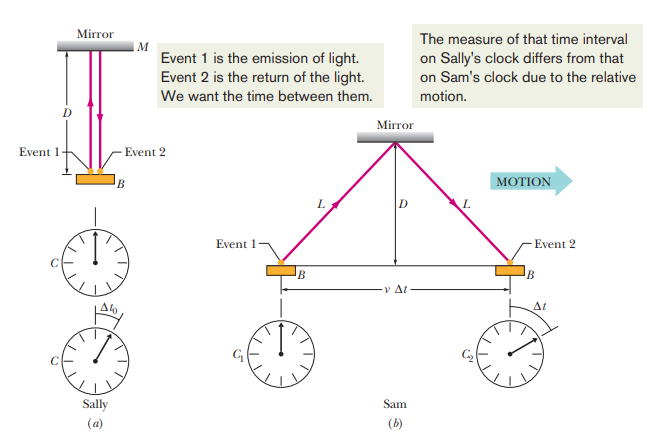
\includegraphics[scale=0.5]{Bild_2023-01-29_225326706.png}
    \captionsetup{textformat=empty,labelformat=blank}
    \caption{Lichtuhr}
\end{figure}

a) zeigt die vereinfachte Version des Experiments, welches Sally, unser Beobachter, durchführt währenddessen, sie, ihre Ausrüstung, eine Lichtquelle, ein Spiegel und eine Uhr auf einem Zug fahren und sich mit der konstanten Geschwindigkeit $\vec{v}$ relativ zur Station bewegen. Eine Lichtwelle verlässt die Quelle $B$ (Ereignis 1) und bewegt sich vertikal nach oben und wird dort wiederum nach unten reflektiert durch den Spiegel. Unten angekommen wird es durch die Quelle (Ereignis 2) wieder wahrgenommen. Das Zeitinterval $\delta t_0$ zwischen den beiden Ereignissen ist logischerweise abhängig von der Distanz $D$ zwischen Quelle $B$ und Spiegel. Das Zeitinterval
\begin{equation}
\Delta t_0 = \frac{2D}{c} (Sally)\label{egn: t 1.0}\tag{t.1.0}
\end{equation}
Die beiden Ereignisse finden am selben Ort statt und in Sally's Bezugssystem. Sie braucht nur eine Uhr $C$ um das Zeitinterval zu messen.

Nun betrachten wir die beiden Ereignisse aus der Perspektive von Sam, welcher auf der Plattform steht, während der Zug vorbei fährt. Da der Zug und die Messausrüstung sich bewegt sieht Sam den Weg den der Lichtstrahl zurücklegt anders als Sally. Siehe Fig.b). In seinem Bezugssystem finden die beiden Ereignisse an unterschiedlichen Orten statt und somit muss Sam zwei Uhren $C_1$ und $C_2$ verwenden welche miteinander synchronisiert sind, um das Zeitinterval zwischen den beiden Ereignissen messen zu können. Aufgrund von Einsteins zweitem Postulat bewegt sich das Licht in allen Inertialsystemen mit derselben Geschwindigkeit. Aufgrund der Tatsache, dass sich der Zug relativ zur Plattform bewegt, hat das Licht einen anderen Weg als zuvor innerhalb des Zugs. Die zurückgelegte Länge ist somit länger als die vorherige. Wir bezeichnen die Länge der Quelle $B$ zum Spiegel nun mit $L$. Es ergibt sich nun folgende Gleichung für das Zeitinterval aus dem Bezugssystem von Sam
\begin{equation}
\Delta t = \frac{2L}{c} (Sam) \label{egn: t 1.1}\tag{t.1.1}
\end{equation}
Lösen wir nun nach $L$ mit Hilfe von Pythagoras auf, erhalten wir die folgende Gleichung für $L$
\begin{equation}
    L = \sqrt{(\frac{1}{2}v \Delta t)^2 + D^2}\label{egn: t 1.2}\tag{t.1.2}
\end{equation}
Lösen wir nun $\delta t_0$ nach $D$ auf und setzen dies in unsere Gleichung für $L$ ein erhalten wir nun folgendes für unsere Länge $L$
\begin{equation}
    L = \sqrt{(\frac{1}{2}v \Delta t)^2 + \frac{1}{2}c \Delta t_0)^2}\label{egn: t 1.3}\tag{t.1.3}
\end{equation}
Setzen wir nun $L$ in unsere Gleichung für $\Delta t$ ein erhalten wir folgende Gleichung für $\Delta t$
\begin{equation}
    \Delta t = \frac{\Delta t_0}{\sqrt{1 - (v/c)^2}}\label{egn: t 1.4}\tag{t.1.4}
\end{equation}
\cite{University Physics}\cite{Principles of Physics}


\subsubsection{Zeitdilatation und Eigenzeit}\label{ZD}
Aus letzterer Gleichung erhalten wir eine wichtige Erkenntnis. Aus der Tatsache, dass wir uns nicht schneller als Lichtgeschwindigkeit bewegen können, lässt sich folgende Beziehung zwischen $v$ und $c$ darlegen. $v < c$ was sich auch dadurch beweisen lässt, da $\sqrt{-1} = i$ und man somit Lösungen mit imaginären Zahlen erhalten würde. Aus der Beziehung lässt sich wiederum darlegen, dass $\Delta t > \Delta t_0$ sein muss. Dies ist wiederum auch logisch, da mehr Zeit vergeht um die Distanz $L$ hinter sich zu legen. Es entsteht somit ein interessantes Phänomen. Die vergangene Zeit zwischen den beiden Ereignissen ist unterschiedlich von Inertialsystem zu Inertialsystem. Dies lässt sich dadurch erklären, dass Licht ein Eigen-Vektor und somit invariant in fast allen Systemen ist. Genau diese Änderung des Zeitintervals nennt man Zeitdilatation. Wir schliessen daraus, dass die relative Bewegung eines Inertialsystems einen Einfluss auf die wahrgenommene Zeit hat. \cite{University Physics}\cite{Principles of Physics} Das Textbuch-Beispiel verdeutlicht nebst der Zeitdilatation noch etwas anderes. Aufgrund von dem Textbeispiel und seinen Ergebnissen, lässt sich ein neuer Term für das Zeitinterval in dem Inertialsystem bilden, in welchem die beiden Ereignisse stattfinden, nämlich Eigenzeit. Einfach gesagt spricht man von Eigenzeit, wenn man sich in seinem eigenen Inertialsystem befindet und bspw. eine Arbeit schreibt, genau dann erfährt man die sogenannte Eigenzeit, welche nun in einem stationären Bezugssystem stattfindet. Wenn man ein Zeitinveral mit dem Eigenzeitinterval vergleicht und das Zeitinterval grösser ist als das Eigenzeitinterval, dann wird von der, wie schon erwähnten, Zeitdilatation gesprochen. \cite{Principles of Physics}

Aufgrund von unserem kurzen Textbuch-Beispiel lässt sich auch auf den Lorentzfaktor schliessen.

Der Faktor ist ersichtlich aus der letzteren Gleichung für $\Delta t$. Es ist nämlich genau der Faktor, um welchen sich $\Delta t_0$ von $\Delta t$, unterscheidet.

\begin{equation}
    \gamma = \frac{1}{\sqrt{1 - (v/c)^2}}\label{egn: t 1.5}\tag{t.1.5}
\end{equation}

Zur Veranschaulichung der stärke der Veränderung von $\Delta t$, abhängig von der Geschwindigkeit folgt eine Grafik.

\begin{figure}[h!]
    \captionsetup{textformat=empty, labelformat=blank}
    \caption{$\beta \gamma-Diagramm$}
    \begin{tikzpicture}

\definecolor{darkgray176}{RGB}{176,176,176}
\definecolor{green}{RGB}{0,128,0}

\begin{axis}[
tick align=outside,
tick pos=left,
title={\(\displaystyle \beta \gamma\) Wert Gegenüberstellung },
x grid style={darkgray176},
xlabel={\(\displaystyle \beta\)},
xmajorgrids,
xmin=0, xmax=1,
xtick style={color=black},
y grid style={darkgray176},
ylabel={\(\displaystyle \gamma\)},
ymajorgrids,
ymin=0, ymax=10,
ytick style={color=black},
axis lines = left
]
\addplot [semithick, green]
table {%
0 1
0.001 1.00000050000037
0.002 1.000002000006
0.003 1.00000450003038
0.004 1.000008000096
0.005 1.00001250023438
0.006 1.00001800048601
0.007 1.00002450090041
0.008 1.00003200153608
0.009 1.00004050246054
0.01 1.00005000375031
0.011 1.00006050549093
0.012 1.00007200777693
0.013 1.00008451071188
0.014 1.00009801440835
0.015 1.00011251898794
0.016 1.00012802458124
0.017 1.00014453132792
0.018 1.00016203937663
0.019 1.00018054888508
0.02 1.00020006002001
0.021 1.00022057295719
0.022 1.00024208788145
0.023 1.00026460498666
0.024 1.00028812447575
0.025 1.00031264656071
0.026 1.00033817146259
0.027 1.00036469941152
0.028 1.00039223064669
0.029 1.00042076541639
0.03 1.00045030397799
0.031 1.00048084659795
0.032 1.00051239355185
0.033 1.00054494512434
0.034 1.00057850160924
0.035 1.00061306330945
0.036 1.00064863053702
0.037 1.00068520361313
0.038 1.00072278286811
0.039 1.00076136864145
0.04 1.00080096128179
0.041 1.00084156114697
0.042 1.00088316860397
0.043 1.000925784029
0.044 1.00096940780745
0.045 1.00101404033391
0.046 1.00105968201221
0.047 1.0011063332554
0.048 1.00115399448578
0.049 1.00120266613488
0.05 1.00125234864352
0.051 1.00130304246176
0.052 1.00135474804897
0.053 1.00140746587381
0.054 1.00146119641423
0.055 1.00151594015753
0.056 1.00157169760033
0.057 1.00162846924857
0.058 1.00168625561759
0.059 1.00174505723207
0.06 1.00180487462608
0.061 1.00186570834309
0.062 1.00192755893598
0.063 1.00199042696707
0.064 1.00205431300809
0.065 1.00211921764024
0.066 1.0021851414542
0.067 1.0022520850501
0.068 1.00232004903762
0.069 1.0023890340359
0.07 1.00245904067364
0.071 1.00253006958909
0.072 1.00260212143005
0.073 1.0026751968539
0.074 1.00274929652762
0.075 1.0028244211278
0.076 1.00290057134066
0.077 1.00297774786208
0.078 1.00305595139758
0.079 1.00313518266238
0.08 1.00321544238141
0.081 1.0032967312893
0.082 1.00337905013043
0.083 1.00346239965895
0.084 1.00354678063875
0.085 1.00363219384357
0.086 1.00371864005692
0.087 1.00380612007217
0.088 1.00389463469256
0.089 1.00398418473117
0.09 1.00407477101102
0.091 1.00416639436502
0.092 1.00425905563604
0.093 1.00435275567692
0.094 1.00444749535046
0.095 1.00454327552949
0.096 1.00464009709686
0.097 1.00473796094548
0.098 1.00483686797834
0.099 1.00493681910851
0.1 1.00503781525921
0.101 1.0051398573638
0.102 1.0052429463658
0.103 1.00534708321894
0.104 1.00545226888717
0.105 1.00555850434468
0.106 1.00566579057593
0.107 1.0057741285757
0.108 1.00588351934907
0.109 1.00599396391147
0.11 1.00610546328873
0.111 1.00621801851707
0.112 1.00633163064312
0.113 1.00644630072401
0.114 1.00656202982732
0.115 1.00667881903116
0.116 1.00679666942419
0.117 1.00691558210561
0.118 1.00703555818527
0.119 1.0071565987836
0.12 1.00727870503173
0.121 1.00740187807143
0.122 1.00752611905525
0.123 1.00765142914644
0.124 1.00777780951905
0.125 1.00790526135794
0.126 1.00803378585882
0.127 1.00816338422826
0.128 1.00829405768375
0.129 1.00842580745371
0.13 1.00855863477755
0.131 1.00869254090566
0.132 1.00882752709948
0.133 1.00896359463153
0.134 1.00910074478542
0.135 1.00923897885593
0.136 1.00937829814898
0.137 1.00951870398172
0.138 1.00966019768254
0.139 1.00980278059113
0.14 1.00994645405847
0.141 1.01009121944691
0.142 1.0102370781302
0.143 1.01038403149349
0.144 1.01053208093343
0.145 1.01068122785815
0.146 1.01083147368732
0.147 1.01098281985222
0.148 1.01113526779571
0.149 1.01128881897234
0.15 1.01144347484835
0.151 1.0115992369017
0.152 1.01175610662215
0.153 1.01191408551128
0.154 1.01207317508251
0.155 1.01223337686118
0.156 1.01239469238458
0.157 1.01255712320196
0.158 1.01272067087463
0.159 1.01288533697594
0.16 1.01305112309138
0.161 1.0132180308186
0.162 1.01338606176742
0.163 1.01355521755995
0.164 1.01372549983056
0.165 1.01389691022599
0.166 1.01406945040533
0.167 1.01424312204012
0.168 1.01441792681437
0.169 1.01459386642462
0.17 1.01477094257997
0.171 1.01494915700216
0.172 1.01512851142556
0.173 1.01530900759729
0.174 1.01549064727723
0.175 1.01567343223805
0.176 1.01585736426531
0.177 1.01604244515747
0.178 1.01622867672597
0.179 1.01641606079524
0.18 1.01660459920281
0.181 1.0167942937993
0.182 1.01698514644852
0.183 1.01717715902751
0.184 1.01737033342658
0.185 1.01756467154937
0.186 1.01776017531291
0.187 1.01795684664769
0.188 1.01815468749766
0.189 1.01835369982035
0.19 1.0185538855869
0.191 1.01875524678211
0.192 1.0189577854045
0.193 1.01916150346637
0.194 1.01936640299387
0.195 1.01957248602704
0.196 1.01977975461988
0.197 1.01998821084039
0.198 1.02019785677068
0.199 1.02040869450696
0.2 1.02062072615966
0.201 1.02083395385347
0.202 1.02104837972739
0.203 1.02126400593482
0.204 1.02148083464359
0.205 1.02169886803606
0.206 1.02191810830915
0.207 1.02213855767442
0.208 1.02236021835816
0.209 1.0225830926014
0.21 1.02280718266002
0.211 1.02303249080482
0.212 1.02325901932154
0.213 1.02348677051099
0.214 1.02371574668907
0.215 1.02394595018687
0.216 1.02417738335072
0.217 1.02441004854228
0.218 1.02464394813857
0.219 1.02487908453211
0.22 1.02511546013091
0.221 1.02535307735863
0.222 1.02559193865456
0.223 1.02583204647379
0.224 1.02607340328719
0.225 1.02631601158157
0.226 1.02655987385969
0.227 1.02680499264039
0.228 1.0270513704586
0.229 1.02729900986549
0.23 1.02754791342852
0.231 1.02779808373148
0.232 1.02804952337464
0.233 1.02830223497477
0.234 1.02855622116526
0.235 1.02881148459617
0.236 1.02906802793434
0.237 1.02932585386346
0.238 1.02958496508416
0.239 1.02984536431406
0.24 1.03010705428791
0.241 1.03037003775765
0.242 1.03063431749247
0.243 1.03089989627895
0.244 1.03116677692109
0.245 1.03143496224045
0.246 1.0317044550762
0.247 1.03197525828524
0.248 1.03224737474227
0.249 1.03252080733987
0.25 1.03279555898864
0.251 1.03307163261725
0.252 1.03334903117252
0.253 1.03362775761957
0.254 1.03390781494187
0.255 1.03418920614137
0.256 1.03447193423853
0.257 1.03475600227252
0.258 1.03504141330121
0.259 1.03532817040137
0.26 1.03561627666867
0.261 1.03590573521786
0.262 1.03619654918284
0.263 1.03648872171676
0.264 1.03678225599213
0.265 1.0370771552009
0.266 1.03737342255461
0.267 1.03767106128446
0.268 1.03797007464143
0.269 1.03827046589638
0.27 1.03857223834016
0.271 1.03887539528373
0.272 1.03917994005825
0.273 1.03948587601522
0.274 1.03979320652654
0.275 1.04010193498469
0.276 1.04041206480278
0.277 1.04072359941473
0.278 1.04103654227531
0.279 1.04135089686032
0.28 1.04166666666667
0.281 1.04198385521251
0.282 1.04230246603737
0.283 1.04262250270224
0.284 1.04294396878972
0.285 1.04326686790411
0.286 1.0435912036716
0.287 1.04391697974032
0.288 1.0442441997805
0.289 1.04457286748459
0.29 1.0449029865674
0.291 1.04523456076622
0.292 1.04556759384093
0.293 1.04590208957415
0.294 1.04623805177138
0.295 1.04657548426113
0.296 1.04691439089501
0.297 1.04725477554794
0.298 1.04759664211822
0.299 1.0479399945277
0.3 1.04828483672192
0.301 1.04863117267022
0.302 1.04897900636593
0.303 1.04932834182646
0.304 1.04967918309348
0.305 1.05003153423303
0.306 1.0503853993357
0.307 1.05074078251677
0.308 1.05109768791633
0.309 1.05145611969946
0.31 1.05181608205636
0.311 1.05217757920253
0.312 1.05254061537887
0.313 1.05290519485189
0.314 1.05327132191383
0.315 1.05363900088284
0.316 1.05400823610313
0.317 1.0543790319451
0.318 1.05475139280554
0.319 1.05512532310779
0.32 1.05550082730187
0.321 1.05587790986469
0.322 1.05625657530017
0.323 1.05663682813943
0.324 1.05701867294099
0.325 1.05740211429086
0.326 1.0577871568028
0.327 1.05817380511843
0.328 1.05856206390745
0.329 1.05895193786778
0.33 1.05934343172574
0.331 1.05973655023628
0.332 1.06013129818308
0.333 1.06052768037881
0.334 1.06092570166525
0.335 1.06132536691352
0.336 1.06172668102425
0.337 1.06212964892776
0.338 1.06253427558427
0.339 1.06294056598409
0.34 1.06334852514778
0.341 1.0637581581264
0.342 1.06416947000165
0.343 1.06458246588611
0.344 1.06499715092343
0.345 1.06541353028853
0.346 1.06583160918778
0.347 1.06625139285927
0.348 1.06667288657292
0.349 1.0670960956308
0.35 1.06752102536725
0.351 1.06794768114914
0.352 1.06837606837607
0.353 1.0688061924806
0.354 1.06923805892844
0.355 1.06967167321871
0.356 1.07010704088413
0.357 1.07054416749124
0.358 1.07098305864068
0.359 1.07142371996735
0.36 1.07186615714068
0.361 1.07231037586484
0.362 1.07275638187902
0.363 1.07320418095758
0.364 1.0736537789104
0.365 1.07410518158303
0.366 1.07455839485697
0.367 1.0750134246499
0.368 1.07547027691597
0.369 1.07592895764599
0.37 1.07638947286771
0.371 1.07685182864608
0.372 1.0773160310835
0.373 1.07778208632007
0.374 1.07825000053387
0.375 1.07871977994119
0.376 1.07919143079683
0.377 1.07966495939436
0.378 1.08014037206637
0.379 1.08061767518476
0.38 1.08109687516103
0.381 1.08157797844651
0.382 1.0820609915327
0.383 1.0825459209515
0.384 1.08303277327553
0.385 1.08352155511841
0.386 1.08401227313503
0.387 1.08450493402187
0.388 1.08499954451729
0.389 1.08549611140182
0.39 1.08599464149846
0.391 1.086495141673
0.392 1.08699761883432
0.393 1.08750207993468
0.394 1.08800853197005
0.395 1.08851698198045
0.396 1.08902743705022
0.397 1.08953990430836
0.398 1.09005439092888
0.399 1.0905709041311
0.4 1.09108945117996
0.401 1.09161003938642
0.402 1.09213267610774
0.403 1.09265736874782
0.404 1.09318412475758
0.405 1.09371295163529
0.406 1.0942438569269
0.407 1.0947768482264
0.408 1.09531193317622
0.409 1.09584911946752
0.41 1.09638841484059
0.411 1.09692982708522
0.412 1.09747336404108
0.413 1.09801903359803
0.414 1.09856684369658
0.415 1.09911680232822
0.416 1.09966891753582
0.417 1.10022319741402
0.418 1.10077965010958
0.419 1.10133828382187
0.42 1.10189910680315
0.421 1.10246212735908
0.422 1.10302735384904
0.423 1.10359479468662
0.424 1.10416445833996
0.425 1.10473635333221
0.426 1.10531048824197
0.427 1.10588687170366
0.428 1.10646551240799
0.429 1.10704641910241
0.43 1.1076296005915
0.431 1.10821506573746
0.432 1.10880282346052
0.433 1.10939288273944
0.434 1.1099852526119
0.435 1.11057994217504
0.436 1.11117696058585
0.437 1.11177631706171
0.438 1.11237802088079
0.439 1.1129820813826
0.44 1.11358850796843
0.441 1.11419731010188
0.442 1.1148084973093
0.443 1.11542207918033
0.444 1.11603806536838
0.445 1.11665646559118
0.446 1.11727728963122
0.447 1.11790054733637
0.448 1.1185262486203
0.449 1.11915440346308
0.45 1.11978502191171
0.451 1.12041811408062
0.452 1.12105369015225
0.453 1.1216917603776
0.454 1.12233233507678
0.455 1.12297542463956
0.456 1.12362103952597
0.457 1.12426919026684
0.458 1.12491988746442
0.459 1.12557314179292
0.46 1.12622896399914
0.461 1.12688736490306
0.462 1.12754835539841
0.463 1.12821194645335
0.464 1.12887814911102
0.465 1.12954697449021
0.466 1.13021843378594
0.467 1.13089253827017
0.468 1.13156929929237
0.469 1.13224872828021
0.47 1.13293083674021
0.471 1.13361563625839
0.472 1.13430313850098
0.473 1.13499335521504
0.474 1.13568629822919
0.475 1.13638197945427
0.476 1.13708041088408
0.477 1.13778160459605
0.478 1.13848557275196
0.479 1.13919232759868
0.48 1.13990188146888
0.481 1.14061424678178
0.482 1.14132943604388
0.483 1.14204746184974
0.484 1.14276833688272
0.485 1.14349207391573
0.486 1.14421868581207
0.487 1.14494818552615
0.488 1.14568058610432
0.489 1.14641590068567
0.49 1.14715414250283
0.491 1.1478953248828
0.492 1.14863946124777
0.493 1.14938656511599
0.494 1.15013665010256
0.495 1.15088972992034
0.496 1.1516458183808
0.497 1.15240492939488
0.498 1.1531670769739
0.499 1.15393227523044
0.5 1.15470053837925
0.501 1.15547188073816
0.502 1.15624631672903
0.503 1.15702386087862
0.504 1.15780452781964
0.505 1.15858833229162
0.506 1.15937528914189
0.507 1.16016541332661
0.508 1.16095871991171
0.509 1.16175522407388
0.51 1.16255494110166
0.511 1.16335788639635
0.512 1.16416407547315
0.513 1.16497352396214
0.514 1.16578624760936
0.515 1.16660226227788
0.516 1.1674215839489
0.517 1.16824422872279
0.518 1.16907021282027
0.519 1.16989955258347
0.52 1.17073226447712
0.521 1.17156836508963
0.522 1.17240787113429
0.523 1.17325079945047
0.524 1.17409716700473
0.525 1.17494699089209
0.526 1.17580028833721
0.527 1.17665707669563
0.528 1.177517373455
0.529 1.17838119623635
0.53 1.17924856279538
0.531 1.18011949102368
0.532 1.18099399895013
0.533 1.18187210474214
0.534 1.18275382670699
0.535 1.18363918329325
0.536 1.18452819309204
0.537 1.18542087483849
0.538 1.18631724741313
0.539 1.18721732984325
0.54 1.18812114130439
0.541 1.18902870112178
0.542 1.18994002877177
0.543 1.19085514388335
0.544 1.19177406623964
0.545 1.19269681577941
0.546 1.19362341259863
0.547 1.194553876952
0.548 1.19548822925454
0.549 1.19642649008321
0.55 1.1973686801785
0.551 1.19831482044605
0.552 1.19926493195834
0.553 1.20021903595635
0.554 1.20117715385125
0.555 1.20213930722612
0.556 1.20310551783772
0.557 1.2040758076182
0.558 1.20505019867689
0.559 1.20602871330216
0.56 1.20701137396317
0.561 1.20799820331178
0.562 1.20898922418441
0.563 1.20998445960389
0.564 1.21098393278146
0.565 1.21198766711865
0.566 1.21299568620928
0.567 1.21400801384146
0.568 1.21502467399959
0.569 1.21604569086643
0.57 1.21707108882515
0.571 1.21810089246144
0.572 1.21913512656565
0.573 1.22017381613491
0.574 1.22121698637535
0.575 1.22226466270428
0.576 1.22331687075246
0.577 1.22437363636634
0.578 1.22543498561036
0.579 1.22650094476929
0.58 1.22757154035059
0.581 1.22864679908679
0.582 1.22972674793792
0.583 1.23081141409394
0.584 1.23190082497726
0.585 1.23299500824523
0.586 1.23409399179271
0.587 1.23519780375464
0.588 1.23630647250869
0.589 1.23742002667788
0.59 1.23853849513327
0.591 1.23966190699674
0.592 1.24079029164369
0.593 1.24192367870588
0.594 1.24306209807428
0.595 1.2442055799019
0.596 1.24535415460675
0.597 1.24650785287478
0.598 1.24766670566291
0.599 1.248830744202
0.6 1.25
0.601 1.25117450484505
0.602 1.25235429080865
0.603 1.25353939024885
0.604 1.25472983581352
0.605 1.25592566044368
0.606 1.25712689737681
0.607 1.25833358015025
0.608 1.25954574260464
0.609 1.26076341888744
0.61 1.26198664345644
0.611 1.26321545108336
0.612 1.26444987685748
0.613 1.26568995618936
0.614 1.26693572481455
0.615 1.26818721879741
0.616 1.26944447453498
0.617 1.27070752876085
0.618 1.27197641854915
0.619 1.27325118131858
0.62 1.27453185483645
0.621 1.27581847722289
0.622 1.27711108695498
0.623 1.27840972287105
0.624 1.27971442417501
0.625 1.2810252304407
0.626 1.28234218161639
0.627 1.28366531802927
0.628 1.28499468039003
0.629 1.28633030979756
0.63 1.28767224774359
0.631 1.28902053611756
0.632 1.29037521721146
0.633 1.29173633372475
0.634 1.29310392876939
0.635 1.29447804587492
0.636 1.29585872899364
0.637 1.29724602250584
0.638 1.29863997122511
0.639 1.30004062040379
0.64 1.30144801573838
0.641 1.30286220337521
0.642 1.304283229916
0.643 1.30571114242368
0.644 1.30714598842816
0.645 1.30858781593232
0.646 1.31003667341795
0.647 1.31149260985193
0.648 1.3129556746924
0.649 1.31442591789505
0.65 1.31590338991954
0.651 1.31738814173601
0.652 1.31888022483168
0.653 1.32037969121753
0.654 1.32188659343517
0.655 1.32340098456372
0.656 1.32492291822686
0.657 1.3264524486
0.658 1.32798963041752
0.659 1.32953451898015
0.66 1.33108717016251
0.661 1.33264764042066
0.662 1.33421598679992
0.663 1.33579226694273
0.664 1.3373765390966
0.665 1.33896886212232
0.666 1.34056929550216
0.667 1.34217789934833
0.668 1.3437947344115
0.669 1.34541986208947
0.67 1.34705334443603
0.671 1.34869524416995
0.672 1.35034562468406
0.673 1.35200455005459
0.674 1.35367208505055
0.675 1.35534829514339
0.676 1.35703324651675
0.677 1.35872700607636
0.678 1.36042964146016
0.679 1.36214122104857
0.68 1.36386181397495
0.681 1.36559149013623
0.682 1.3673303202037
0.683 1.36907837563403
0.684 1.37083572868047
0.685 1.37260245240423
0.686 1.37437862068606
0.687 1.37616430823807
0.688 1.3779595906157
0.689 1.37976454422995
0.69 1.38157924635981
0.691 1.3834037751649
0.692 1.38523820969835
0.693 1.38708262991995
0.694 1.38893711670941
0.695 1.39080175188002
0.696 1.39267661819246
0.697 1.39456179936884
0.698 1.39645738010712
0.699 1.39836344609564
0.7 1.40028008402801
0.701 1.40220738161827
0.702 1.4041454276163
0.703 1.40609431182351
0.704 1.40805412510888
0.705 1.41002495942522
0.706 1.4120069078258
0.707 1.41400006448123
0.708 1.41600452469676
0.709 1.41802038492976
0.71 1.42004774280768
0.711 1.42208669714625
0.712 1.42413734796805
0.713 1.42619979652149
0.714 1.4282741453001
0.715 1.43036049806217
0.716 1.43245895985085
0.717 1.43456963701459
0.718 1.43669263722796
0.719 1.43882806951295
0.72 1.44097604426059
0.721 1.44313667325308
0.722 1.44531006968634
0.723 1.44749634819297
0.724 1.44969562486568
0.725 1.45190801728126
0.726 1.45413364452489
0.727 1.45637262721512
0.728 1.45862508752918
0.729 1.46089114922889
0.73 1.46317093768716
0.731 1.46546457991486
0.732 1.46777220458844
0.733 1.47009394207795
0.734 1.47242992447576
0.735 1.47478028562581
0.736 1.47714516115347
0.737 1.4795246884961
0.738 1.48191900693413
0.739 1.4843282576229
0.74 1.48675258362513
0.741 1.48919212994407
0.742 1.49164704355736
0.743 1.49411747345169
0.744 1.49660357065805
0.745 1.49910548828789
0.746 1.50162338157001
0.747 1.50415740788819
0.748 1.50670772681975
0.749 1.50927450017489
0.75 1.51185789203691
0.751 1.51445806880329
0.752 1.51707519922776
0.753 1.5197094544632
0.754 1.5223610081056
0.755 1.52503003623893
0.756 1.52771671748107
0.757 1.53042123303077
0.758 1.53314376671565
0.759 1.53588450504133
0.76 1.53864363724166
0.761 1.54142135533015
0.762 1.54421785415251
0.763 1.54703333144049
0.764 1.54986798786695
0.765 1.55272202710216
0.766 1.55559565587154
0.767 1.55848908401463
0.768 1.56140252454559
0.769 1.56433619371503
0.77 1.56729031107337
0.771 1.57026509953575
0.772 1.57326078544841
0.773 1.5762775986568
0.774 1.57931577257528
0.775 1.58237554425847
0.776 1.5854571544745
0.777 1.58856084777993
0.778 1.59168687259657
0.779 1.59483548129024
0.78 1.59800693025148
0.781 1.60120147997827
0.782 1.60441939516085
0.783 1.6076609447687
0.784 1.61092640213971
0.785 1.61421604507165
0.786 1.61753015591602
0.787 1.62086902167422
0.788 1.62423293409636
0.789 1.62762218978252
0.79 1.63103709028671
0.791 1.63447794222359
0.792 1.637945057378
0.793 1.64143875281732
0.794 1.64495935100699
0.795 1.64850717992896
0.796 1.65208257320343
0.797 1.6556858702139
0.798 1.65931741623553
0.799 1.66297756256713
0.8 1.66666666666667
0.801 1.67038509229062
0.802 1.67413320963713
0.803 1.67791139549314
0.804 1.68172003338575
0.805 1.68555951373776
0.806 1.68943023402761
0.807 1.69333259895396
0.808 1.6972670206049
0.809 1.70123391863208
0.81 1.70523372042986
0.811 1.70926686131966
0.812 1.71333378473973
0.813 1.71743494244049
0.814 1.7215707946856
0.815 1.72574181045909
0.816 1.72994846767862
0.817 1.73419125341513
0.818 1.73847066411919
0.819 1.74278720585417
0.82 1.74714139453653
0.821 1.75153375618356
0.822 1.75596482716867
0.823 1.76043515448469
0.824 1.76494529601533
0.825 1.76949582081524
0.826 1.77408730939883
0.827 1.77872035403838
0.828 1.78339555907152
0.829 1.78811354121877
0.83 1.7928749299112
0.831 1.79768036762884
0.832 1.80253051025014
0.833 1.80742602741287
0.834 1.81236760288707
0.835 1.81735593496038
0.836 1.82239173683623
0.837 1.82747573704554
0.838 1.83260867987234
0.839 1.83779132579394
0.84 1.84302445193621
0.841 1.84830885254459
0.842 1.85364533947147
0.843 1.85903474268072
0.844 1.86447791076982
0.845 1.86997571151071
0.846 1.87552903240978
0.847 1.88113878128802
0.848 1.88680588688219
0.849 1.89253129946781
0.85 1.898315991505
0.851 1.90416095830811
0.852 1.91006721874028
0.853 1.91603581593387
0.854 1.92206781803807
0.855 1.92816431899481
0.856 1.93432643934429
0.857 1.94055532706147
0.858 1.94685215842488
0.859 1.95321813891933
0.86 1.95965450417405
0.861 1.96616252093787
0.862 1.97274348809324
0.863 1.97939873771095
0.864 1.98612963614738
0.865 1.9929375851865
0.866 1.99982402322859
0.867 2.00679042652812
0.868 2.01383831048314
0.869 2.0209692309787
0.87 2.02818478578709
0.871 2.03548661602769
0.872 2.04287640768942
0.873 2.05035589321909
0.874 2.05792685317899
0.875 2.06559111797729
0.876 2.07335056967508
0.877 2.08120714387416
0.878 2.08916283168973
0.879 2.09721968181269
0.88 2.1053798026663
0.881 2.11364536466235
0.882 2.12201860256239
0.883 2.13050181794972
0.884 2.13909738181845
0.885 2.14780773728619
0.886 2.1566354024374
0.887 2.1655829733049
0.888 2.17465312699757
0.889 2.18384862498276
0.89 2.19317231653256
0.891 2.20262714234367
0.892 2.21221613834125
0.893 2.22194243967798
0.894 2.23180928494032
0.895 2.24182002057454
0.896 2.25197810554656
0.897 2.26228711625004
0.898 2.27275075167863
0.899 2.28337283887941
0.9 2.29415733870562
0.901 2.30510835188833
0.902 2.31623012544829
0.903 2.32752705947047
0.904 2.339003714266
0.905 2.35066481794787
0.906 2.36251527444891
0.907 2.37456017201296
0.908 2.38680479219252
0.909 2.39925461938901
0.91 2.41191535097474
0.911 2.42479290803892
0.912 2.43789344680378
0.913 2.45122337076059
0.914 2.46478934358006
0.915 2.47859830285599
0.916 2.49265747474662
0.917 2.50697438958366
0.918 2.52155689852566
0.919 2.53641319133918
0.92 2.55155181539914
0.921 2.56698169600847
0.922 2.58271215814657
0.923 2.59875294976697
0.924 2.61511426677618
0.925 2.63180677983908
0.926 2.64884166317073
0.927 2.66623062549104
0.928 2.6839859433368
0.929 2.70212049694631
0.93 2.72064780895472
0.931 2.73958208616384
0.932 2.75893826467959
0.933 2.77873205874238
0.934 2.7989800136131
0.935 2.81969956291876
0.936 2.84090909090909
0.937 2.86262800012895
0.938 2.88487678507225
0.939 2.9076771124523
0.94 2.93105190880275
0.941 2.95502545621338
0.942 2.97962349710892
0.943 3.00487334909789
0.944 3.03080403105545
0.945 3.05744640176234
0.946 3.0848333126048
0.947 3.11299977605236
0.948 3.14198315187689
0.949 3.17182335336373
0.95 3.20256307610174
0.951 3.23424805233328
0.952 3.26692733430823
0.953 3.30065361063367
0.954 3.33548356025757
0.955 3.37147824949449
0.956 3.40870357841772
0.957 3.44723078403963
0.958 3.48713700901973
0.959 3.52850594622956
0.96 3.57142857142857
0.961 3.61600397864797
0.962 3.66234033574207
0.963 3.71055598108363
0.964 3.76078068672103
0.965 3.81315711870399
0.966 3.8678425320109
0.967 3.92501074595819
0.968 3.98485445664586
0.969 4.04758795657246
0.97 4.11345034894863
0.971 4.18270936669223
0.972 4.25566593530122
0.973 4.3326596571309
0.974 4.41407544535133
0.975 4.50035160370409
0.976 4.59198973981653
0.977 4.68956702499546
0.978 4.7937514864377
0.979 4.90532126007065
0.98 5.02518907629605
0.981 5.15443374703602
0.982 5.29434114991496
0.983 5.44645829170019
0.984 5.61266568833672
0.985 5.79527587799745
0.986 5.99717000347998
0.987 6.22199116787736
0.988 6.47442474054589
0.989 6.76061595262364
0.99 7.08881205008335
0.991 7.47038724839213
0.992 7.92155313155596
0.993 8.46637168460183
0.994 9.14243324231049
0.995 10.0125234864352
0.996 11.1915370258961
0.997 12.9196378521231
0.998 15.8192999292083
0.999 22.3662720421294
};
\end{axis}

\end{tikzpicture}

\end{figure}
\newpage
Die Grafik zeigt den Verlauf des Lorentzfaktors verglichen mit dem $\beta$-Wert, dabei ist $\beta = v/c$. Es ist nun ersichtlich, dass der Wert des Lorentzfaktors $\gamma$ sich dem unendlichen nähert, sobald sich der $\beta$-Wert 1 annähert. Dies ist logisch, da wir uns nach unseren Gesetzen der Physik nicht schneller als Lichtgeschwindigkeit bewegen können und somit stellt die Lichtgeschwindigkeit die ultimative Grenze aller Geschwindigkeiten dar. Mathematisch lässt sich die Grafik aufgrund der Tatsache erklären, dass wir $\sqrt{-1}$ nicht im kartesischen Koordinatensystem darstellen können und die Lösung für uns somit nicht greifbar ist.
\cite{Principles of Physics}


Es ist nun ersichtlich, dass sich unsere Gleichung für $\Delta t $ nun folgendermassen umschreiben lässt\cite{Principles of Physics}
\begin{equation*}
    \Delta t = \gamma \Delta t
\end{equation*} 



\subsubsection{Längenkontraktion}\label{LK}
Wie auch bei der Zeit oder besser gesagt den Intervallen der Zeit zwischen mehreren Ereignissen hat das Konzept der Relativität auch einen Einfluss auf die Länge. Wie im Abschnitt zur Zeit bereits erklärt wurde, hat der Abstand zwischen den verschiedenen Inertialsystemen auch einen Einfluss auf die Zeit, die vom jeweiligen Beobachter wahrgenommen wird. Somit ist die Konsequenz daraus, dass die wahrgenommene Länge in verschiedenen Inertialsystemen unterschiedlich sein kann. Besser gesagt ist die Längenkontraktion ein direkte Schlussfolgerung der Zeitdilatation. \cite{Principles of Physics} Um den Zusammenhang besser verständlich zu machen, lässt sich folgendes Beispiel nehmen. Man stelle sich vor man wolle die Länge eines sich bewegenden Fahrzeugs bestimmen. Dazu braucht man zwei Personen, welche jeweils die Front und das Heck des Fahrzeug gleichzeitig markieren. Genau hierbei liegt nun das Problem, denn wie im Abschnitt zur Gleichzeitigkeit etabliert, ist diese kein absolutes Konzept und ist von Beobachter zu Beobachter verschieden. Genau dies führt dazu, dass einer unserer Assistenten, sein jeweiliges Teil des Fahrzeugs, nicht zur selben Zeit wie der Andere markiert und wir so die wahre Länge des bewegten Fahrzeugs nicht ermitteln können. \cite{University Physics} 

Genau wie schon bei der Relativität der Zeiten lässt sich auch hier nun wieder das gleiche Konzept der Eigenzeit und des wahrgenommenen Zeitintervals aus der Perspektive eines sich geradlinig-gleichförmigen bewegenden Beobachters wiederaufnehmen. Nun heisst das Konzept der Eigenzeit bei Längen Eigenlänge. Genau diese werden wir nun versuchen herzuleiten. \cite{Principles of Physics} \cite{University Physics} Dazu wollen wir nun wiederum ein Gedankenexperiment durchführen. Wir nehmen an, dass wir ein Rohr haben an welchen an einem Ende eine Lichtquelle befestigt ist und am anderen Ende ein Spiegel. Wir beobachten dieses Rohr aus dem Inertialsystem, welches wir $S$ nennen und das Rohr selbst befindet sich im Inertialsystem $S'$ und hat dort die Länge $L_0$. Man sieht schon die Parallelen zu unserem vorherigen Gedankenexperiment zur Bestimmung der Eigenzeit. Nun wollen wir der Dauer, welche vergeht wenn man das Licht aussendet und dann am Spiegel abprallt und wieder zurückkehrt einen Namen geben, wir nennen dieses Zeitintervall $\Delta t_0$.\cite{Principles of Physics} \cite{University Physics}
\begin{equation}
    \Delta t_0 = \frac{2 L_0}{c} \label{eqn: lc 1.0} \tag{l.0}
\end{equation}
Welches uns aus dem vorherigen Experiment zur Eigenzeit bekannt sein sollte. Dieses Zeitintervall ist ein Eigenzeitinterval, da wie bei dem Gedankenexperiment mit der Uhr am selben Ort, auch hier die beiden Ereignisse, Absenden des Lichts und Empfangen des Lichts, im selben Inertialsystem $S'$ stattfinden. \cite{University Physics}
Wir nehmen nun an, dass sich dieses Rohr in seinem Inertialsystem $S'$ nach Rechts mit der Geschwindigkeit $v$ bewegt. Aus Sicht unseres Beobachters im Inertialsystem $S$ hat unser Rohr die Länge $L$ und das Zeitintervall, welches vergeht, wenn das Licht von der Quelle zum Spiegel ausbreitet, entspricht $\Delta t_1$. Während dieses Zeitintervalls bewegt sich das Rohr eine Strecke $v \cdot \Delta t_1$ nach der herkömlichen Formel $s = v \cdot t$. Es gilt nun nicht mehr $L_0 = L$. Die Länge von der Quelle bis zu unserem Spiegel ist nun
\begin{equation}
    d = L + v \Delta t_1 \label{eqn: lc 1.1}\tag{l.1}
\end{equation}
\cite{University Physics}
Da sich Licht mit der selben Geschwindigkeit in allen Inertialsystem bewegt, lässt sich folgende Gleichung für $d$ aufstellen
\begin{equation}
    d = c \Delta t_1 \label{eqn: lc 1.2}\tag{l.2}
\end{equation}
Wenn wir nun \ref{eqn: lc 1.1} gleichsetzen mit \ref{eqn: lc 1.2} erhalten wir
\begin{align}
    c \Delta t_1 &= L + v \Delta t_1 \notag \\
    c &= \frac{L}{\Delta t_1} + v\notag\\
    c - v &= \frac{L}{\Delta t_1}\notag\\
    \frac{1}{c-v} &= \frac{\Delta t_1}{L}\notag\\
    \Delta t_1 &= \frac{L}{c - v} \label{eqn: lc 1.3}\tag{l.3}
\end{align}
Das bedeutet nun logischerweise, dass das Licht in $S$ weiter ausbreitet als die Länge $L$ unseres Rohres. Daraus können wir schliessen, wenn die Distanz hin länger ist, dann muss sie zurück kürzer sein. Daher ergibt sich die folgende Gleichung für das Intervall Spiegel Quelle
\begin{equation}
    \Delta t_2 = \frac{L}{c + v} \label{eqn: lc 1.4}\tag{l.4}
\end{equation}
Die gesamte Zeit, welche im Inertialsystem $S$ des Beobachters vergeht entspricht $\Delta t = \Delta t_1 + \Delta t_2$ \cite{University Physics}
\begin{align}
    \Delta t &= \frac{L}{c - v} + \frac{L}{c + v}\notag\\
    &= \frac{L(c+v)+L(c-v)}{(c-v)(c+v)} \notag\\
    &= \frac{L(2c)}{(c-v)(c+v)}\notag\\
    &= \frac{2L\cdot c}{c^2 - v^2}\notag\\
    &= \frac{2L \cdot c/c}{c-\frac{v^2}{c}}\notag\\
    &= \frac{2L}{c(1-\frac{v^2}{c^2})}\label{eqn: lc 1.5}\tag{l.5}
\end{align}
Wir wissen, dass $\Delta t$ und $\Delta t_0$ einen Zusammenhang haben aus der Gleichung \ref{egn: t 1.4}. Wenn wir nun \ref{egn: t 1.4} nach $\Delta t_0$ umformen erhalten wir
\begin{equation}
    \Delta t_0 = \Delta t \sqrt{1-\frac{v^2}{c^2}} \label{eqn: lc 1.6}\tag{l.6}
\end{equation}
Zusätzlich wissen wir noch, dass $\Delta t_0$ einer Eigenzeit in $S'$ entspricht und wir somit auf folgende Gleichung für das Interval hin und zurück $\Delta t_0$ schliessen können
\begin{equation}
    \Delta t \sqrt{1 - \frac{v^2}{c^2}} = \frac{2L_0}{c} \label{eqn: lc 1.7}\tag{l.7}
\end{equation}
Nun setzen wir \ref{eqn: lc 1.5} in \ref{eqn: lc 1.7} ein
\begin{equation*}
    \frac{2L}{c(1-\frac{v^2}{c^2})}\cdot \sqrt{1 - \frac{v^2}{c^2}} = \frac{2L_0}{c}
\end{equation*}
let $z = 1 - \frac{v^2}{c^2}$
\begin{align}
    \frac{l}{z}\cdot \sqrt{z} &= L_0 \notag\\
    L \cdot \sqrt{z} &= L_0 \cdot z \notag\\
    L^2 \cdot z &= {L_0}^2 \cdot z^2 \notag\\
    L^2 &= {L_0}^2 \cdot \frac{z^2}{z} \notag\\
    L &= L_0 \cdot \sqrt{z} \notag\\
    L &= L_0 \cdot \sqrt{1-\frac{v^2}{c^2}} = \frac{L_0}{\gamma} \label{eqn: lc 1.8}\tag{l.8}
\end{align}
\cite{University Physics}
Nun haben wir bewiesen, dass $L$ in $S$ kürzer ist als $L_0$ in $S'$. Daraus folgt nun unsere Definition der Eigenlänge. Die Eigenlänge wird definiert als die Länge im unbewegten System, daraus folgt dass $t_0$ der Eigenlänge in $S'$ entspricht. Daraus folgt dass alle Längen, welche ausserhalb von $S'$ gemessen werden kürzer sind als $L_0$ um den Faktor $\gamma^-1$. Diesen Effekt nennt man Längenkontraktion. \cite{University Physics}

Dies war nun die Herleitung der Gleichung für Längen, welche sich in paralleler Richtung zum Beobachter bewegen. Für Objekte welche orthogonal stehen zur relativen Bewegung gilt, dass sie in allen System erhalten bleiben, sie werden also nicht kontrahiert.


\subsection{Mathematische Hintergründe}
\subsubsection{Minkowski-Raum}
Hier ist nur eine kurze Erklärung der Grundlagen des Minkowski-Raumes. Es wird nicht all zu tief darauf eingegangen, sondern nur das Wichtigste erklärt, welches später bei der Herleitung der Lorentztransformation wichtig ist.
Minkowski-Raum ist ein Konzept, welches durch den Physiker Hermann Minkowski erschaffen wurde für die Maxwell Gleichung zum Elektromagnetismus \cite{Minkowski Space}. Minkowski-Raum vereinigt den dreidimensionalen euklidischen Raum und Zeit in eine 4 dimensionale Mannigfaltigkeit. In diesem Konzept werden nur die euklidischen Koordinaten und Zeitkoordinaten durch Zeitdilatation und Längenkontraktion verändert. In diesem Konzept sind sich alle Inertialsysteme aufgrund von Einsteins Postulaten der Lichtgeschwindigkeit und der Erhaltung der physikalischen Gesetze in allen Inertialsystemen, einig über den Raumzeit Abstand von zwei Ereignissen unabhängig von deren Inertialsystem. Minkowski geht von einem 4 dimensionalen Koordinatensystem mit den Koordinaten des 4er-Vektors, dazu in einem späteren Kapitel mehr, $\Vec{x} = (x,y,z,ct)$.
Angenommen, dass unsere Raumzeit flach ist, erhalten wir die folgende Gleichung unter der Annahme, dass wir uns in $R^4$ befinden und die folgende Metrik für flache Raumzeit gilt.
\cite{Minkowski Space}
\begin{equation*}
\eta_{\mu\nu} = \begin{bmatrix}
    -c^2 &  0 & 0 & 0\\
     0 & 1 & 0 & 0 \\
     0 & 0 & 1 & 0 \\
     0 & 0 & 0 & 1
\end{bmatrix}
\end{equation*}
Dabei ist anzumerken, dass diese Metrik sich im Rahmen der speziellen Relativitätstheorie nicht ändert, da wir von einer Flachen Raumzeit ausgehen. Die Metrik $\eta$ ändert sich jedoch in der Generellen Relativitätstheorie von Ort zu Ort, da wir dort von einer gekrümmten Raumzeit ausgehen.

Es gilt die folgende Gleichung:
\begin{equation*}
    ds^2 = -c^2dt^2 + dx^2 + dy^2 + dz^2
\end{equation*}

Diese Gleichung gilt aufgrund des Längenquadrates des kontravariante und des kovarianten Vektors. Dieses Gesetz lässt sich aus dem Lichtausbreitungsgesetz \ref{L3} herleiten, da jenes eigentlich die Invarianz der 4er-Vektoren aufgrund von \ref{L2} beweist.


\paragraph{Minkowski Diagramme}
Minkowski Diagramme entsprechen der grafischen Darstellung des zuvor Beschriebenen und sind elementar in der Herleitung der Lorentztransformationen und der Darstellung von verschiedenen Paradoxen-Verhaltensweisen, welche sich aus der speziellen Relativitätstheorie ergeben. \cite{Minkowski Diagrams}

\begin{figure}[h!]
    \captionsetup{textformat=empty, labelformat=blank}
    \caption{Minkowski-Diagramm}
    \begin{tikzpicture}
        \tkzInit[xmax=2,ymax=2,xmin=-2,ymin=-2]
        \tkzAxeXY
        \draw[ thick,latex-latex] (-2,-1) -- (2,1) node[anchor=south west] {$x'$}; % two points for drawing 2x+y=2
        \draw[ thick,latex-latex] (-1,-2) -- (1,2) node[anchor=south west] {$ct'$}; % two points for drawing 2x+y=2
        \tkzText[above](0,4){Minkowski-Diagramm}
    \end{tikzpicture}
\end{figure}
Die wichtigste Annahme, welche in unseren Minkowski Diagrammen gelten muss, ist diejenige der invarianten Lichtgeschwindigkeit über alle Inertialsysteme hinweg. Dies funktioniert nur, wenn die Lichtgeschwindigkeit mit einem 45 Grad Winkel zu den beiden Achsen verläuft und so eine Symmetrie bildet. Ausserdem muss das Licht linear verlaufen, da es konstant bleiben muss. Es lässt sich nun folgende Symmetrie grafisch erkennen. Genau diese Symmetrie der Koordinaten-Achsen Verschiebung wird mit den Lorentz-Transformationen beschrieben. 
\begin{center}

\newpage

\begin{figure}
\captionsetup{textformat=empty, labelformat=blank}
\caption{Lorentz-Transformation Koordinatensystem}
\begin{tikzpicture}

% This command generates a Minkowski space diagram.
% 
% Parameter 1: width of 1 grid space
% Parameter 2: maximum x/ct value
% Parameter 3: proportion of speed of light
\newcommand{\spacetimediagram}[3]{
    % Draw the x and ct axes
    \draw[<->,thick] (-#2*#1-#1, 0) -- (#2*#1+#1, 0);
    \draw[<->,thick] (0, -#2*#1-#1) -- (0, #2*#1+#1);
    % Draw the x ct grid
    \draw[step=#1,gray,very thin] (-#2*#1, -#2*#1) grid (#2*#1, #2*#1);

    % Evaluate the Lorentz transformation
    \FPeval{\calcgamma}{1/((1-(#3)^2)^.5)}
    \FPeval{\calcbetagamma}{\calcgamma*#3}

    % Draw the x' and ct' axes
    \draw[<->,thick,cm={\calcgamma,\calcbetagamma,\calcbetagamma,\calcgamma,(0,0)},blue] (-#2*#1-#1, 0) -- (#2*#1+#1, 0);
    \draw[<->,thick,cm={\calcgamma,\calcbetagamma,\calcbetagamma,\calcgamma,(0,0)},blue] (0, -#2*#1-#1) -- (0, #2*#1+#1);

    % Draw the vertical transformed grid lines
    \foreach \x in {-#2,...,#2}
        \draw[cm={\calcgamma,\calcbetagamma,\calcbetagamma,\calcgamma,(0,0)},blue,very thin] (\x*#1,-#2*#1) -- (\x*#1,#2*#1);
    % Draw the horizontal transformed grid lines
    \foreach \y in {-#2,...,#2}
        \draw[cm={\calcgamma,\calcbetagamma,\calcbetagamma,\calcgamma,(0,0)},blue,very thin] (-#2*#1,\y*#1) -- (#2*#1,\y*#1);

    % Draw the x and ct axes labels
    \draw (#2*#1+#1+0.2,0) node {$x$};
    \draw (0,#2*#1+#1+0.2) node {$ct$};
    % Draw the x' and ct' axes labels
    \draw[cm={\calcgamma,\calcbetagamma,\calcbetagamma,\calcgamma,(0,0)},blue] (#2*#1+#1+0.2,0) node {$x^\prime$};
    \draw[cm={\calcgamma,\calcbetagamma,\calcbetagamma,\calcgamma,(0,0)},blue] (0,#2*#1+#1+0.2) node {$ct^\prime$};
    
    % Draw the unit indicators
    \draw (#2*#1+0.34,-0.26) node {$\qty{#2}{\m}$};
    \draw (-0.33,#2*#1+0.3) node {$\qty{#2}{\m}$};
}
\spacetimediagram{.5}{8}{1/2}
\end{tikzpicture}
\end{figure}
\end{center}
Es lässt sich durch die Grafik somit erkennen, dass es sich bei Licht um einen Eigenvektor handeln muss, denn wenn wir eine Linie bei 45 Grad zur x-Achse plotten scheint die Linie auch beschreibbar durch das blaue Koordinatensystem zu sein. Licht ist nun also wie nach Einsteins Postulat invariant in allen Inertialsystemen und der Minkowski Raum erfüllt somit Einsteins $Postulate$. 

\newpage

\section{Entwicklung des Codes zur Simulation bewegter Objekte}
Da die Grundlagen der linearen Algebra sowie die Grundlagen der speziellen Relativitätstheorie nun klar sind, können wir diese schön verpackt in einem Programm anwenden.

\subsection{Lorentz-Transformationen}
Um bewegte Objekte in Python zu simulieren, müssen wir erstmals die Lorentz-Transformation numerisch in Python implementieren.

\lstset{language=Python}
\lstset{frame=lines}
\lstset{caption={Lorentz-Transformation}}
\lstset{label={lst:LT1}}
\lstset{basicstyle=\footnotesize}
\begin{lstlisting}
import numpy as np

def LorentzTransformation(v,covector): #boostet den Vektor covector mit der Geschwindigkeit v

        c = 1 #c := 100% der Lichtgeschwindigkeit

        gamma = 1/np.sqrt(1-(v**2/c**2)) #Lorentz-Faktor

        beta = v / c # beta

        B = np.array([[gamma, -gamma*beta, 0, 0], # LorentzTransformation
        [-gamma*beta,gamma,0,0],
        [0,0,1,0],
        [0,0,0,1]])

        return np.matmul(B, covector)
\end{lstlisting}

Dabei nimmt der $covector$ einen 4er-Vektor $\begin{pmatrix} ct \\ x \\ y \\ z \end{pmatrix}$ auf und $v$ entspricht der Geschwindigkeit angenommen, dass die Lichtgeschwindigkeit $c = 1$ entspricht. 

Die Funktion Lorentz-Transformation(v,covector) macht dabei genau dasselbe was wir von Hand berechnen würden. Von Hand würden wir genau gleich wie in der Funktion den 4er-Vektor mit der Matrix Form der Lorentz-Transformation boosten. Der Vorteil an numerischen Methoden ist jedoch, dass wir sie nur einmal definieren müssen und dann nur noch andere Datenpunkte in sie einsetzen können.

Den Boost B mit welchem wir unseren covector boosten ist jedoch nur indirekt abhängig von der Geschwindigkeit und verwendet somit nicht die $\mathbf{R}^3$ Geschwindigkeit. Daraus lässt sich schliessen, dass unsere Transformation $B$ nicht ganz genau ist oder nur einer Näherung entspricht. Möchten wir nun die zuvor erwähnten Ungenauigkeiten beheben erhalten wir folgendes Programm.


\lstset{language=Python}
\lstset{frame=lines}
\lstset{caption={Lorentz-Transformation}}
\lstset{label={lst:LT2}}
\lstset{basicstyle=\footnotesize}
\begin{lstlisting}
import numpy as np

def LorentzBoost(vvector,covector): 
# Boostet den Vektor covector unter der Bedingung des Geschwindigkeitsvektors vvector

        v_x = vvector[0]
        v_y = vvector[1]
        v_z = vvector[2]
        

        v = np.sqrt(v_x**2 + v_y**2 + v_z**2)

        c = 1 #c := 100% der Lichtgeschwindigkeit

        gamma = 1/np.sqrt(1-(v**2/c**2))

        B = np.array([[gamma, ((-gamma*v_x)/c), ((-gamma*v_y)/c), ((-gamma*v_z)/c)],
                      [((-gamma*v_x)/c), (1 + ((gamma-1)*(((v_x**2))/v**2))), 
                      
                      ((gamma-1)*((v_x*v_y)/v**2)), ((gamma-1)*((v_x*v_z)/v**2))],
                      
                      [((-gamma*v_y)/c), ((gamma-1)*((v_y*v_x)/v**2)), 
                      
                      (1 + ((gamma-1)*(((v_y**2))/v**2))) , ((gamma-1)*((v_y*v_z)/v**2))],
                      
                      [((-gamma*v_z)/c), ((gamma-1)*((v_z*v_x)/v**2)), ((gamma-1)*((v_z*v_y)/v**2)),
                      (1 + ((gamma-1)*(((v_z**2))/v**2)))]])

        return np.matmul(B, covector)
\end{lstlisting}

Man sieht nun, dass wir die Geschwindigkeit auch als Array aufnehmen und nicht mehr als Konstante. Da wir die Geschwindigkeit $v$ als Konstante ebenfalls benötigen, müssen wir die Norm des Geschwindigkeitsvektors $vvector$ nehmen in dem wir $\sqrt{(v_x)^2 + (v_y)^2 + (v_z)^2}$ ziehen. Nun ist unser $\gamma$ auch abhängig von den $\mathbf{R}^3$ Koordinaten unserens Geschwindigkeitsvektors. Das Array $B$ kann nun, wie im Code gezeigt, angepasst werden. Das Resultat der Funktion bleibt gleich, da wir nur den Boost verändert haben und die Grundstruktur erhalten bleibt.


\subsection{Simulation des Gesehenen}
Nun da wir den Code für die Lorentz-Transformationen etabliert haben, können wir beginnen den Code zur Beobachtung eines Objekts zu programmieren. Denn nur unsere Lorentz-Transformationen selber bringen uns noch nicht soviel, da wir nicht das Gesehene programmieren würden, sondern dass was das Objekt tatsächlich macht. Dies kann jedoch von uns nicht wahrgenommen werden, da Licht eine bestimmte Zeit braucht, um bei uns anzukommen. Ausserdem spielt der räumliche Abstand zwischen zwei Inertialsystemen nun auch eine Rolle, da wir uns nicht mehr im gleichen Inertialsystem befinden. Wir nehmen nun an, dass es ein Inertialsystem $S'$, in dem sich der Beobachter befindet, gibt und ein Inertialsystem $S$, in dem das Ereignis stattfindet. Das Inertialsystem $S$ bewegt sich dabei gradlinig-gleichförmig mit der Geschwindigkeit $v$ relativ zu unserem Beobachtersystem.

Mathematisch müssen wir nun folgendes tun, um das Tatsächliche in das Wahrgenommene umzuwandeln.


Man boostet den Vierervektor $x = \begin{pmatrix} 
x^0 \\ x^1 \\ x^2 \\ x^3
\end{pmatrix}
 = \begin{pmatrix}
    \lambda \\ x^1 \\ x^2 \\ x^3
\end{pmatrix}$
,wobei $\lambda$ der Raumzeitkoordinate entspricht, mit dem Lorentz-Boost $B$ $:=$ \ref{L17} in das Inertialsystem $S'$.

\begin{equation}\label{csm1}
    x' = \mathbf{B}x = \begin{pmatrix}
        \lambda \\ x^1 \\ x^2 \\ x^3
    \end{pmatrix} \begin{bmatrix}
        \gamma & -\gamma \beta & 0 & 0\\
        -\gamma \beta & \gamma & 0 & 0 \\
        0 & 0 & 1 & 0 \\
        0 & 0 & 0 & 1
    \end{bmatrix} = \begin{bmatrix}
        \gamma \lambda - \beta \gamma x^1 \\ -\beta \gamma \lambda + \gamma x^1 \\ x^2 \\ x^3
    \end{bmatrix} \tag{csm.1}
\end{equation}
\begin{equation*}
    x' =  \begin{pmatrix}
        \lambda' \\ {x^1}' \\ {x^2}' \\ {x^3}' 
    \end{pmatrix} \notag
\end{equation*}
Man bestimmt nun einen Beobachter in $S'$ $O = \begin{pmatrix}
    O^0 \\ O^1 \\ O^2 \\ O^3
\end{pmatrix}$
von welchem wir den Abstand der Raumkoordinaten, ohne die Raumzeitkoordinate, zwischen $O$ und $x' \backslash \lambda'$ berechnen. Dies tun wir indem wir die Norm dieses Abstandsvektors nehmen.

\begin{equation}\label{csm.2}
    d = ||\Vec{x'} - \Vec{O}|| = \sqrt{({x_1}'-O_1)^2 + ({x_2}'-O_2)^2 + ({x_3}'-O_3)^2} \tag{csm.2}
\end{equation}
Nun benötigen wir für unsere Simulation jedoch wieder die Zeitkoordinate also stellen wir folgende Gleichung für unser $\tau$ in unserem Beobachter $O$ auf.
\begin{equation}\label{csm.3}
    \tau = \lambda' + \frac{d}{c} = \gamma \lambda - \beta \gamma x^1 + \frac{d}{c} \tag{csm.3}
\end{equation}

Nun müssen wir jedoch nach $\lambda'$ umformen, da wir in unserer Gleichung nach dem Zeitpunkt im Inertialsystem $S$ suchen, weil wir im Beobachtersystem die Zeit variieren und nun eigentlich die Zeit im System des Objekts, welches sich bewegt, haben möchten. Diesen neuen Vektor wollen wir mit dem nun bekannten $\lambda$ ins Beobachtersystem boosten, um die wahre Position in $S'$ zu erhalten. 

\lstset{language=Python}
\lstset{frame=lines}
\lstset{caption={Boost}}
\lstset{label={lst:Boost}}
\lstset{basicstyle=\footnotesize}
\begin{lstlisting}
import numpy as np
from scipy.optimize import fsolve

def functiontosolve(lam,tau,x,y,vvector): 
#Diese Funktion muss 0 sein, damit das Teilchen den Beobachter zum Zeitpunkt tau trifft

    x = np.array([lam[0],x[0],x[1],x[2]]) #position Teilchen
    o = np.array([tau,y[0],y[1],y[2]]) #position Beobachter
    xP = LorentzBoost(v_vector,x) #position des Licht-Teilchens im Beobachtersystem

    s = np.subtract(xP,o) #Vektor x' und o

    d = np.linalg.norm(s[1:]) #Abstand zwischen x' und o

    return(d+xP[0]-tau) #return die Funktion, welche 0 sein muss, sodass das Licht den Beobachter zum Zeitpunkt tau trifft

def LorentzBoost(vvector,covector): # Boostet den Vektor covector unter der Bedingung des Geschwindigkeitsvektors vvector

        v_x = vvector[0]
        v_y = vvector[1]
        v_z = vvector[2]
        

        v = np.sqrt(v_x**2 + v_y**2 + v_z**2)

        c = 1 #c := 100% der Lichtgeschwindigkeit

        gamma = 1/np.sqrt(1-(v**2/c**2))

        B = np.array([[gamma, ((-gamma*v_x)/c), ((-gamma*v_y)/c), ((-gamma*v_z)/c)],
                      [((-gamma*v_x)/c), (1 + ((gamma-1)*(((v_x**2))/v**2))), 
                      
                      ((gamma-1)*((v_x*v_y)/v**2)), ((gamma-1)*((v_x*v_z)/v**2))],
                      
                      [((-gamma*v_y)/c), ((gamma-1)*((v_y*v_x)/v**2)), 
                      
                      (1 + ((gamma-1)*(((v_y**2))/v**2))) , ((gamma-1)*((v_y*v_z)/v**2))],
                      
                      [((-gamma*v_z)/c), ((gamma-1)*((v_z*v_x)/v**2)), ((gamma-1)*((v_z*v_y)/v**2)),
                      (1 + ((gamma-1)*(((v_z**2))/v**2)))]])

        return np.matmul(B, covector)


def Transform(x,y,vvector,tau):     
#x: Position des Objekts in seinem Inertialsystem, y: position des Beobachters
#v_vector: Geschwindigkeit des Inertialsystems relativ zum Beobachter, tau: Zeit beim Beobachter
    lam = fsolve(functiontosolve,x0=tau,args=(tau,x,y,vvector))  #berechnet die roots der Funktion functiontosolve

    x = np.array([lam[0],x[0],x[1],x[2]]) #Licht-Teilchen zur Zeit lambda im bewegten System
    xP = LorentzBoost(vvector,x) #boost zurueck ins Beobachtersystem

    #print(f"lambda = {lam1}; x = {x}; xP = {xP}")

    return xP
\end{lstlisting}
$functionsolve$ gibt eine Funktion heraus, welche nach 0 aufgelöst wird, um so die verschiedenen möglichen Parameter zur Lösung der Gleichung $\lambda' + \frac{d}{c} -\tau = 0$ mit $c = 1$ zu bestimmen. Die Funktion LorentzBoost \ref{csm1} gibt das Produkt von Boost und x zurück. Die Transform nimmt die Position des Objekts, die Position des Beobachters, den Geschwindigkeitsvektor und den Zeitpunkt $\tau$ auf. Dabei ist $\tau$ spezifisch als eigener Parameter gewählt worden, um später bei den Simulationen verschiedene Werte für $\tau$ als Input geben zu können. $lam$ berechnet die möglichen Lösungs-Werte der Funktion $functionsolve$. $x$ verwendet man zur Berechnung von $x'$ im Beobachtersystem mit nun berechnetem Wert für $\lambda$. 

\vspace{1cm}

Zur Überprüfung der Richtigkeit unseres Programms wollen wir nun einen Beobachter und einen Punkt, welcher sich mit einer bestimmten Geschwindigkeit relativ zum Beobachter bewegt, bestimmen und in unser Programm füttern, sowie von Hand berechnen. Bspw. 
\begin{itemize}
    \item Beobachter o := $\begin{pmatrix}
        0 \\ 10 \\ 0
    \end{pmatrix}$
    \item Punkt x := $\begin{pmatrix}
        1 \\ 1 \\ 1
    \end{pmatrix}$
    \item v := $\begin{pmatrix}
        0.95 \\ 0 \\ 0
    \end{pmatrix}$
\end{itemize}

Mit der definierten Funktion zum Zeitpunkt $\tau = 1$ $Transform(Punkt, Beobachter, Geschwindigkeit, Zeit)$

Zuerst führen wir die Berechnung mit unserem \textbf{Programm} \ref{lst:Boost} durch, da wir es ja auf seine Richtigkeit prüfen wollen.
\lstset{language=Python}
\lstset{frame=lines}
\lstset{caption={Überprüfung}}
\lstset{label={lst:uberprufung}}
\lstset{basicstyle=\footnotesize}
\begin{lstlisting}
import numpy as np
from scipy.optimize import fsolve

def Transform(x,y,v_vector,tau):     
#x: Position des Objekts in seinem Inertialsystem, y: position des Beobachters
#v_vector: Geschwindigkeit des Inertialsystems relativ zum Beobachter, tau: Zeit beim Beobachter
    lam = fsolve(functiontosolve,x0=tau,args=(tau,x,y,v_vector))  #berechnet die roots der Funktion functiontosolve

    x = np.array([lam[0],x[0],x[1],x[2]]) #Licht-Teilchen zur Zeit lambda im bewegten System
    xP = LorentzBoost(v_vector,x) #boost zurueck ins Beobachtersystem

    #print(f"lambda = {lam1}; x = {x}; xP = {xP}")

    return xP

x = np.array([1,1,1]) # Punkt
o = np.array([0,10,0]) # Beobachter
v = np.array([0.95,0,0]) # Geschwindigkeit
tau = 1

xP = Transform(x,o,v,tau)

print(xP)
\end{lstlisting}
Wir erhalten $[-22.51497808 ; 21.70147907 ; 1.00000000 ; 1.00000000]$.
Nun wollen wir dasselbe von Hand durchführen:
Zuerst berechnen wir die norm des Geschwindigkeitsvektors
\begin{equation*}
    ||v|| = \sqrt{0.95^2} = 0.95
\end{equation*}
Dann berechnen wir den Lorentzfaktor
\begin{equation*}
    \gamma = \frac{1}{\sqrt{1-0.95^2}}
\end{equation*}

Nun bestimmen wir $x'$ mit den gegebenen Daten für $\gamma$ und $v$
\begin{align*}
    x' &= 
    \begin{bmatrix}
        \gamma & -\gamma v_x / c & -\gamma v_y / c & -\gamma v_z / c \\
        -\gamma v_x / c & 1 + (\gamma -1)\frac{{v_x}^2}{v^2} & (\gamma -1)\frac{v_x v_y}{v^2} & (\gamma -1)\frac{v_x v_z}{v^2} \\
        -\gamma v_y / c & (\gamma -1)\frac{v_y v_x}{v^2} & 1 + (\gamma -1)\frac{{v_y}^2}{v^2} & (\gamma -1)\frac{v_y v_z}{v^2} \\
        -\gamma v_z / c & (\gamma -1)\frac{v_z v_x}{v^2} & (\gamma -1)\frac{v_z v_y}{v^2} & 1 + (\gamma -1)\frac{{v_z}^2}{v^2}
    \end{bmatrix} \cdot \begin{pmatrix}
        \lambda \\ 1 \\ 1 \\ 1
    \end{pmatrix} \\
    &= \begin{bmatrix}
        \frac{1}{\sqrt{1-0.95^2}} & - \frac{0.95}{\sqrt{1-0.95^2}} & 0 & 0 \\
        - \frac{0.95}{\sqrt{1-0.95^2}} & \frac{1}{\sqrt{1-0.95^2}} & 0 & 0 \\
        0 & 0 & 1 & 0 \\
        0 & 0 & 0 & 1
    \end{bmatrix} \cdot \begin{pmatrix}
        \lambda \\ 1 \\ 1 \\ 1
    \end{pmatrix} \\
    &= \begin{pmatrix}
        \frac{\lambda}{\sqrt{1-0.95^2}} - \frac{0.95}{\sqrt{1-0.95^2}} \\
        - \frac{0.95 \cdot \lambda}{\sqrt{1-0.95^2}} + \frac{1}{\sqrt{1-0.95^2}} \\ 1 \\ 1
    \end{pmatrix}
\end{align*}
Nach der Berechnung von $x'$ können wir die Euklidische-Norm von $\Vec{x}' - \Vec{o}$ bestimmen. Das bedeutet die Norm ohne die Raumzeitkoordinate.
\begin{align*}
    \overrightarrow{ox'} &= \begin{pmatrix} - \frac{0.95 \cdot \lambda}{\sqrt{1-0.95^2}} + \frac{1}{\sqrt{1-0.95^2}} \\ 1 \\ 1 \end{pmatrix} - \begin{pmatrix} 0 \\ 10 \\ 0\end{pmatrix} = \begin{pmatrix}  - \frac{0.95 \cdot \lambda}{\sqrt{1-0.95^2}} + \frac{1}{\sqrt{1-0.95^2}} \\ -9 \\ 1\end{pmatrix} \\
    d &= ||\overrightarrow{ox'}|| = \sqrt{(- \frac{0.95 \cdot \lambda}{\sqrt{1-0.95^2}} + \frac{1}{\sqrt{1-0.95^2}})^2 + (-9)^2 + 1^2} = \sqrt{(- \frac{0.95 \cdot \lambda}{\sqrt{1-0.95^2}} + \frac{1}{\sqrt{1-0.95^2}})^2 + 82}
\end{align*}
Wir können nun unsere Ergebnisse in \ref{csm.2} mit $\tau = 1$ einsetzen und erhalten
\begin{align*}
    \tau &= {x_0}' + \frac{d}{c}\\
    1 &= \frac{\lambda}{\sqrt{1-0.95^2}} - \frac{0.95}{\sqrt{1-0.95^2}} + \sqrt{(- \frac{0.95 \cdot \lambda}{\sqrt{1-0.95^2}} + \frac{1}{\sqrt{1-0.95^2}})^2 + 82} \\
\end{align*}

Lösen wir nun nach $\lambda$ auf, erhalten wir $\lambda = -6.0802996510862957034$. Wenn wir dieses $\lambda$ nun in unseren Punkt $x$ einsetzen und den wiederum mit dem Lorentz-Boost bosten erhalten wir
\begin{equation*}
    \begin{pmatrix}
       -22.514978076499 \\ 21.701479072594 \\ 1 \\ 1
    \end{pmatrix}
\end{equation*}
Wir erhalten also den selben Vektor. Dies beweist somit, dass unser Programm richtig ist.

Nun haben wir ein funktionierendes Programm, dass einen Punkt zu einem bestimmten Zeitpunkt $\tau$ transformieren kann und in das Beobachtersystem boosten kann. Jetzt wollen wir ein Programm schreiben, welches den Punkt für mehrere Zeitpunkte boosten kann, damit wir das Vorbeifliegen des Objekts bei relativistischen Geschwindigkeiten beobachten können. 
Dazu brauchen wir nun ein Programm, welches Graphen animieren kann und es erlaubt einen entsprechenden Wert für das $\tau$ für jedes $Frame$ des animierten aufzunehmen und nach dem den Punkt zu boosten. Der bereits ertablierte Code bleibt bestehen. Der folgende Code zeigt nur die Funktion, welche notwendig ist um das Ganze für mehrere $\tau$ zu animieren.

\lstset{language=Python}
\lstset{frame=lines}
\lstset{caption={Animation}}
\lstset{label={lst:Animation}}
\lstset{basicstyle=\footnotesize}
\begin{lstlisting}
import matplotlib.pyplot as plt
import numpy as np
from matplotlib.animation import FuncAnimation

x = np.array([0,0,0])
o = np.array([0,10,0])
v = np.array([0.95,0,0])

fig, ax = plt.subplots()

line, = ax.plot([],[],'o')

def animate(ntau):
    x1_data = Transform(x,o,v,ntau)[1]
    y1_data = Transform(x,o,v,ntau)[3]

    line.set_data([x1_data],[y1_data])

anim = FuncAnimation(fig, animate, frames = 100, interval = 100)
plt.grid()
plt.show()

\end{lstlisting}
Wie man sieht ist nun bei \emph{Transform} anstatt von einer spezifischen Zeit einfach ein Parameter ntau, welcher sich bei $FuncAnimation$ für 100 Frames ändert. Eine wichtige Anmerkung ist, dass wir jeweils nur die x- und die z-Koordinate plotten und nicht die Zeitkoordinate. Dies liegt daran, dass wir schlecht 4D Grafiken darstellen können und im 3D sieht man später bei der Einbeziehung der Perspektive die Veränderung nur schlecht. Eine andere wichtige Bemerkung ist, dass wir aufgrund der Annahme, dass $c=1$ unsere Daten in Lichtsekunden darstellen. Also ein Abstand von 1 bedeutet soviel wie $3\cdot10^8 m$.
Da animieren in LaTeX selbst nur schlecht funktioniert folgt ein Plot, wie es ungefähr aussieht, wenn wir einen Punkt mit den Koordinaten $(0,0,0)$ mit der Geschwindigkeit $(0.95,0,0)$ boosten und von $(0,10,0)$ aus beobachten.

\begin{figure}[h!]
    \centering
    \caption{Punkt animation}
    
        % This file was created with tikzplotlib v0.10.1.
    \begin{tikzpicture}\label{fig:punkt animation}

    \definecolor{darkgray176}{RGB}{176,176,176}
    \definecolor{steelblue31119180}{RGB}{31,119,180}

    \begin{axis}[
    tick align=outside,
    tick pos=left,
    x grid style={darkgray176},
    xmajorgrids,
    xmin=-33.826980361047, xmax=1.54477915887036,
    xtick style={color=black},
    y grid style={darkgray176},
    ymajorgrids,
    ymin=0.945, ymax=1.055,
    ytick style={color=black}
    ]
    \addplot [semithick, steelblue31119180, mark=*, mark size=3, mark options={solid}, only marks]
    table {%
    -32.2191731101416 1
    -22.5149780765 1
    -15.7894155616415 1
    -11.2410518823864 1
    -8.06727731227477 1
    -5.72959681916518 1
    -3.91054356417704 1
    -2.42592440653108 1
    -1.16604488383099 1
    -0.0630280920349744 1
    };
    \end{axis}

    \end{tikzpicture}

\end{figure}
Man sieht hier die Längenkontraktion bereits sehr schön. 
Nun möchten wir noch den sogenannten \textbf{Relativistischen Doppler-Effekt} und die korrekte Perspektive implementieren

\subsection{Relativistischer Doppler-Effekt}
Der relativistische Doppler-Effekt beschreibt das Phänomen der Farbänderung bei relativistischen Geschwindigkeiten relativ zum Beobachter. Es findet somit eine Veränderung der Frequenz und somit der Wellenlänge statt. Im Unterschied zum klassischen Doppler-Effekt muss man hier noch die Folgen der speziellen Relativitätstheorie miteinbeziehen, wie bspw. die Zeitdilatation. \cite{RD}

\newpage
\begin{figure}[h!]
    \centering
    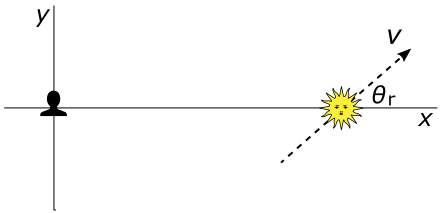
\includegraphics[scale=0.5]{doppler.png}
    \caption{Relativistischer Doppler-Effekt}
    \label{fig:RD}
\end{figure}

Dies Abbildung zeigt den Beobachter beim Koordinaten Ursprung und das Ereignis als Sonne, welches sich mit dem Vektor $\Vec{v}$ in einem Winkel $\theta_r$ zur x-Achse fortbewegt.

Mit einigen Überlegungen fand man, dass folgende Gleichung für die Bewegung in eine beliebige Richtung für die empfangene Frequenz $f_r$ richtig ist.

\begin{equation}\label{rd.1}
    f_r = \frac{f_s}{\gamma (1 + \beta \cos{\theta_r})} \tag{rd.1}
\end{equation}

Wenn wir nun versuchen diese Gleichung für einen beliebigen Beobachter und ein beliebiges Ereignis zu lösen, wird ersichtlich, dass wir den Winkel $\theta_r$ brauchen. Dazu müssen wir erstmals den Vektor zwischen Beobachter und Ereignis bestimmen.
\begin{equation}\label{rd.2}
\overrightarrow{xo} = 
\begin{pmatrix} x^1 - O^1 \\ x^2 - O^2 \\ x^3 - O^3 \end{pmatrix}\tag{rd.2}
\end{equation}

Wenn wir nun $\overrightarrow{xo}$ haben können wir einfach den Winkel zwischen $\overrightarrow{xo}$ und $v$ bestimmen und so auf unseren Winkel $\theta_r$ schliessen.
\begin{equation}\label{rd.3}
    \theta_r = \arccos{\frac{\overrightarrow{xo} \cdot \Vec{v}}{||\overrightarrow{xo}|| ||\Vec{v}||}}\tag{rd.3}
\end{equation} 

\cite{RD}

Wir müssen jetzt nur noch unsere Wellenlänge, welche ausgesendet wird $\lambda_s$ in die ausgesendete Frequenz $f_s$ umwandeln.

Da $f = \frac{c}{\lambda}$ gilt, müssen wir nur noch $\lambda_s$ für $\lambda$ einsetzen und erhalten unsere ausgesendete Frequenz $f_s$. 

Somit lässt sich die Gleichung \ref{rd.1} nach den, jetzt nur allgemein, gegebenen Parametern folgendermassen umformen.

\begin{equation}\label{rd.4}
    f_r = \frac{\frac{c}{\lambda_s}}{\gamma(1 + \frac{||\Vec{v}||\cdot c}{c}\frac{((x^1 - O^1)v_x) + ((x^2 - O^2)v_y) + ((x^3 - O^3)v_z)}{\sqrt{(x^1 - O^1)^2 + (x^2 - O^2)^2 + (x^3 - O^3)^2} \sqrt{{v^2}_x + {v^2}_y + {v^2}_z}}} \tag{rd.4}
\end{equation}

Dieser Prozess ist ersichtlich im folgenden Programm:

\lstset{language=Python}
\lstset{frame=lines}
\lstset{caption={Frequenz}}
\lstset{label={lst:Frequenz}}
\lstset{basicstyle=\footnotesize}
\begin{lstlisting}
import matplotlib.pyplot as plt
import numpy as np
def vlength(x): # x := vektor mit [x1,x2,x3,..,xn] 
    
    vint = 0
    
    for n in range(0,len(x)):
        vint += x[n]**2
    
    vlen = np.sqrt(vint)
    
    return vlen


def vectorbetweenXO(x,o): # x := [x1,x2,x3,x4] objekt Vektor; o := [o1,o2,o3,o4] Beobachter Vektor
    xo = np.subtract(x,o)
    
    return xo

def thetaCalc(xo,v): # xo := [xo1,xo2,xo3,xo4] Vektor zwischen x und o; v := geschwindigkeit des senders
    theta = np.arccos((np.dot(xo,v))/(vlength(xo)*vlength(v)))
    
    return theta

def frequency_received(theta_r,f_s,v_s):# empfangene Frequenz
    c = 3*10**8 # ungefaehr Lichtgeschwindigkeit
    beta = v_s / c #beta notation
    gamma = 1 / np.sqrt((1 - beta**2))
    
    
    f_r = f_s / (gamma*(1 + beta*np.cos(theta_r)))
    
    return f_r

\end{lstlisting}

Im Programm wurde die Funktion $vectorbetweenXO(x,o)$ für die Gleichung \ref{rd.2} verwendet. $thetaCalc(xo,v)$ ist eine Funktion welche die Gleichung \ref{rd.3} numerisch lösen kann. Die letzte Funktion $function\_received(theta_r,f_s,v_s)$ ist nichts anderes als die numerische Lösung der Gleichung \ref{rd.4}.


Da unsere Resultate der Funktionen Frequenzen sind, müssen wir eine Funktion schreiben, welche diese interpretieren kann und dann wieder in ihre entsprechende Wellenlängen umwandeln kann. Darauf folgt eine Funktion, welche die Wellenängen in RGB-Values umwandeln kann.

\lstset{language=Python}
\lstset{frame=lines}
\lstset{caption={Farbe}}
\lstset{label={lst:Farbe}}
\lstset{basicstyle=\footnotesize}
\begin{lstlisting}
def waveToRGB(wave):
    gamma = 0.8
    intensity_max = 1
    
    if wave < 380:
        red, green, blue = 1,1,1
    elif wave < 440:
        red = -(wave - 440) / (440 - 380)
        green, blue = 0, 1
    elif wave < 490:
        red = 0
        green = (wave - 440) / (490 - 440)
        blue = 1
    elif wave < 510:
        red, green = 0, 1
        blue = -(wave - 510) / (510 - 490)
    elif wave < 580:
        red = (wave - 510) / (580 - 510)
        green, blue = 1, 0
    elif wave < 645:
        red = 1
        green = - (wave - 645) / (645 - 580)
        blue = 0
    elif wave <= 780:
        red, green, blue = 1, 0 ,0
    else:
        red, green, blue = 1,1,1
    
    if wave < 380:
        factor = 0
    elif wave < 420:
        factor = 0.3 + 0.7 * (wave - 380) / (420 - 380)
    elif wave < 700:
        factor = 1
    elif wave <= 780:
        factor = 0.3 + 0.7 * (780 - wave) / (780 - 700)
    else:
        factor = 0
    
    def f(c):
        if c == 1:
            return 1
        else:
            return intensity_max * pow(c * factor, gamma)
    
    return f(red), f(green), f(blue)

def colorTransform(col,xo,v_s): 
# Transformiert Wellenlaenge in ihre relative Frequenz, welche dann in die relativ empfangene Frequenz umgewandelt wird => das entsprechende RGB-Value wird aus der Wellenlaenge der empfangenen Frequenz bestimmt und die Wellenlaenge muss in nm angegeben werden
    
    f_s = frequency(col)
    f_r=frequency_received(thetaCalc(xo,relativespeed),f_s,v_s)
    
    newcol = waveToRGB(wavelength(f_r)*10**9)
    
    return newcol

\end{lstlisting}
Die Funktion $colorTransform(col,xo,v_s)$ nimmt die Farbe in $\lambda [nm]$, den Vektor zwischen Beobachter und Ereignis $\overrightarrow{xo}$ und die Geschwindigkeit $v_s$ des Senders auf und transformiert diese in die empfangene Wellenlänge, welche dann aufgrund von der Funktion $waveToRGB(\lambda)$ die Wellenlänge $\lambda$ in ihre RGB-Values umwandelt.

Eine wichtige Anmerkung ist, dass sich unser Objekt in $-v$ bewegt uns wir somit $-v$ in unsere Gleichung einsetzen müssen, da wir uns sonst dem Infrarot-Bereich nähern.

Nun da wir die Farbänderung implementiert haben können wir die korrekte Perspektive noch implementieren. Dazu brauchen wir die Geradengleichung zwischen $o$ und $x$ und die Ebene bei $y = 5$. Wir müssen nun den Schnittpunkt zwischen Gerade und Ebene bestimmen.

\begin{equation}\label{p.1}
    g: \begin{pmatrix} x_1 \\ x_2 \\ x_3\end{pmatrix} + \mu \cdot \begin{pmatrix} O_1 - x_1 \\ O_2 - x_2 \\ O_3 - x_3\end{pmatrix}\tag{p.1}
\end{equation}
Dies ist eine allgemeine Geradengleichung für die Gerade zwischen $o$ und $x$.

Nun bestimmen wir die Ebene $E$ mit dem Normalenvektor $\Vec{n} = \begin{pmatrix} 0 \\ -1 \\ 0 \end{pmatrix}$.
\begin{align}\label{p.2}
    E: ax + by + cz + d = 0 \notag\\
    E: -y + d &= 0 \notag \\
    E: -y + 5 &= 0 \tag{p.2}
\end{align}

\begin{tikzpicture}[scale=2]
 \draw[->] (0,0,0) -- (3,0,0) node[below]{$y$};
 \draw[->] (0,0,0) -- (0,0,3) node[below]{$x$};
 \draw[->] (0,0,0) -- (0,3,0) node[left]{$z$};
 \fill[blue,opacity=0.2] (2,0,0) -- (2,0,2) -- (2,3,2) --  (2,3,0) -- node[midway,right]{$E$} cycle;
\end{tikzpicture}

Nun bestimmen wir den Schnittpunkt $S$ in welchem die Gerade \ref{p.1} die Ebene \ref{p.2} schneidet.
\begin{align}\label{p.3}
    - (x_2 + \mu(O_2 - x_2)) + 5 &= 0 \notag\\
    \mu &= \frac{5 - x_2}{(O_2 - x_2)} \tag{p.3}
\end{align}
Jetzt setzen wir den erhaltenen Wert für $\mu$ in unsere Geradengleichung \ref{p.1} ein.

\begin{equation}\label{p.4}
    S = \begin{pmatrix} x_1 + \frac{(5 - x_2)}{O_2 - x_2}\cdot (O_1 - x_1) \\ 5 \\ x_3 + \frac{(5 - x_2)}{O_2 - x_2}\cdot (O_3 - x_3)\end{pmatrix}\tag{p.4}
\end{equation}
Nun können wir unseren Vektor $S$ \ref{p.4} in unser Programm implementieren. Wir schreiben nun eine Funktion, welche den Abstand zwischen unseren geboosteten Punkte und unserem Beobachter als Input nimmt und diese dann in $S$ einsetzt und uns die korrekte Perspektive wiedergibt.

\lstset{language=Python}
\lstset{frame=lines}
\lstset{caption={Perspektive}}
\lstset{label={lst:perspektive}}
\lstset{basicstyle=\footnotesize}
\begin{lstlisting}
import numpy as np
import matplotlib.pyplot as plt
from matplotlib.animation import FuncAnimation

def realPerspectiveMI(x,o):
    
    s1 = x[0] + ((5-x[1])/(o[1]-x[1]))*(o[0]-x[0])
    s2 = 5
    s3 = x[2] + ((5-x[1])/(o[1]-x[1]))*(o[2]-x[2])

    s = np.array([s1,s2,s3])
    
    
    return s


\end{lstlisting}
Es folgt eine Darstellung zum Unterschied, welchen die Perspektive auf unsere Simulation macht.
\begin{figure}[h!]
    \centering
    	% This file was created with tikzplotlib v0.10.1.
    	% This file was created with tikzplotlib v0.10.1.
    	% This file was created with tikzplotlib v0.10.1.
	\begin{tikzpicture}\label{fig:wP}
	
	\definecolor{darkgray176}{RGB}{176,176,176}
	
	\begin{axis}[
	tick align=outside,
	tick pos=left,
	x grid style={darkgray176},
	xmajorgrids,
	xmin=-25, xmax=20,
	xtick style={color=black},
	y grid style={darkgray176},
	ymajorgrids,
	ymin=-1.5, ymax=1.5,
	ytick style={color=black}
	]
	\addplot [semithick, blue, mark=*, mark size=1.5, mark options={solid}, only marks]
	table {%
	30.4243492229665 0
	30.4623559201373 0.5
	32.1015967949336 0.5
	32.0636374581882 0
	};
	\addplot [semithick, blue, mark=*, mark size=1.5, mark options={solid}, only marks]
	table {%
	22.057701998665 0
	22.0940649916464 0.5
	23.2867919372428 0.5
	23.2499557016867 0
	};
	\addplot [semithick, blue, mark=*, mark size=1.5, mark options={solid}, only marks]
	table {%
	16.1269405915327 0
	16.1594143409135 0.5
	16.9948947951701 0.5
	16.9617074191979 0
	};
	\addplot [semithick, blue, mark=*, mark size=1.5, mark options={solid}, only marks]
	table {%
	11.9611135030391 0
	11.9891932354912 0.5
	12.5813731638512 0.5
	12.5525882648812 0
	};
	\addplot [semithick, blue, mark=*,mark size=1.5, mark options={solid}, only marks]
	table {%
	8.9478604963694 0
	8.97199877641038 0.5
	9.40853455870584 0.5
	9.38379498142243 0
	};
	\addplot [semithick, blue, mark=*, mark size=1.5, mark options={solid}, only marks]
	table {%
	6.66859564542035 0
	6.68948218332618 0.5
	7.02654451416052 0.5
	7.0051700947505 0
	};
	\addplot [semithick, blue, mark=*, mark size=1.5, mark options={solid}, only marks]
	table {%
	4.86429935921363 0
	4.88256811724516 0.5
	5.15440090765065 0.5
	5.13574039367034 0
	};
	\addplot [semithick, blue, mark=*, mark size=1.5, mark options={solid}, only marks]
	table {%
	3.37710727655327 0
	3.39326939648716 0.5
	3.62086736543867 0.5
	3.60438902065768 0
	};
	\addplot [semithick, blue, mark=*, mark size=1.5, mark options={solid}, only marks]
	table {%
	2.10896999616061 0
	2.12342141100976 0.5
	2.31999902264356 0.5
	2.30528951215136 0
	};
	\addplot [semithick, blue, mark=*, mark size=1.5, mark options={solid}, only marks]
	table {%
	0.997108943918763 0
	1.01015408772558 0.5
	1.18430023315636 0.5
	1.17104174162447 0
	};
	\addplot [semithick, blue, mark=*, mark size=1.5, mark options={solid}, only marks]
	table {%
	6.81532085218691e-16 0
	0.0118742764553668 0.5
	0.169353062164951 0.5
	0.157300186325606 0
	};
	\addplot [semithick, blue, mark=*, mark size=1.5, mark options={solid}, only marks]
	table {%
	-0.910687164274621 0
	-0.899799754103098 0.5
	-0.75500316321509 0.5
	-0.766041866299691 0
	};
	\addplot [semithick, blue, mark=*, mark size=1.5, mark options={solid}, only marks]
	table {%
	-1.75483535502262 0
	-1.7447891755947 0.5
	-1.60984455673612 0.5
	-1.62002029505076 0
	};
	\addplot [semithick, blue, mark=*, mark size=1.5, mark options={solid}, only marks]
	table {%
	-2.54675635106848 0
	-2.53743465697348 0.5
	-2.41028329330426 0.5
	-2.41971702873327 0
	};
	\addplot [semithick, blue, mark=*, mark size=1.5, mark options={solid}, only marks]
	table {%
	-3.2969863381238 0
	-3.28829439098395 0.5
	-3.1674065400263 0.5
	-3.17619624016529 0
	};
	\addplot [semithick, blue, mark=*,mark size=1.5, mark options={solid}, only marks]
	table {%
	-4.01343858614974 0
	-4.00529861967347 0.5
	-3.88951587394929 0.5
	-3.89774180908581 0
	};
	\addplot [semithick, blue, mark=*, mark size=1.5, mark options={solid}, only marks]
	table {%
	-4.70216308973488 0
	-4.69451058856749 0.5
	-4.5829408095583 0.5
	-4.59066946036098 0
	};
	\addplot [semithick, blue, mark=*, mark size=1.5, mark options={solid}, only marks]
	table {%
	-5.36785933752562 0
	-5.36064025493581 0.5
	-5.2525859221225 0.5
	-5.25987289573736 0
	};
	\addplot [semithick, blue, mark=*,mark size=1.5, mark options={solid}, only marks]
	table {%
	-6.01423008608227 0
	-6.00739873864005 0.5
	-5.90230705510118 0.5
	-5.90919928738971 0
	};
	\addplot [semithick, blue, mark=*,mark size=1.5, mark options={solid}, only marks]
	table {%
	-6.6442303375598 0
	-6.63774779327694 0.5
	-6.5351752750676 0.5
	-6.54171271346299 0
	};
	\addplot [semithick, blue, mark=*, mark size=1.5, mark options={solid}, only marks]
	table {%
	-7.26024576132081 0
	-7.2540785915994 0.5
	-7.15366549783239 0.5
	-7.15988240200014 0
	};
	\addplot [semithick, blue, mark=*, mark size=1.5, mark options={solid}, only marks]
	table {%
	-7.86422267760627 0
	-7.85834198048939 0.5
	-7.75979355564681 0.5
	-7.76571951366215 0
	};
	\addplot [semithick, blue, mark=*, mark size=1.5, mark options={solid}, only marks]
	table {%
	-8.45776418824737 0
	-8.4521448162562 0.5
	-8.35521732985824 0.5
	-8.36087806024424 0
	};
	\addplot [semithick, blue, mark=*, mark size=1.5, mark options={solid}, only marks]
	table {%
	-9.0422022565376 0
	-9.03682220044722 0.5
	-8.94131241881789 0.5
	-8.94673040964536 0
	};
	\addplot [semithick, blue, mark=*, mark size=1.5, mark options={solid}, only marks]
	table {%
	-9.61865244057743 0
	-9.61349233326926 0.5
	-9.5192294825518 0.5
	-9.52442450527798 0
	};
	\addplot [semithick, blue, mark=*, mark size=1.5, mark options={solid}, only marks]
	table {%
	-10.1880559405288 0
	-10.1830986542025 0.5
	-10.0899382160511 0.5
	-10.0949277421188 0
	};
	\addplot [semithick, blue, mark=*, mark size=1.5, mark options={solid}, only marks]
	table {%
	-10.7512122483583 0
	-10.7464425649953 0.5
	-10.6542614372441 0.5
	-10.6590609784965 0
	};
	\addplot [semithick, blue, mark=*, mark size=1.5, mark options={solid}, only marks]
	table {%
	-11.3088047530589 0
	-11.304209092855 0.5
	-11.2129017785378 0.5
	-11.2175251674251 0
	};
	\addplot [semithick, blue, mark=*,mark size=1.5, mark options={solid}, only marks]
	table {%
	-11.8614210067517 0
	-11.8569872027992 0.5
	-11.7664627821945 0.5
	-11.7709224040087 0
	};
	\addplot [semithick, blue, mark=*,mark size=1.5, mark options={solid}, only marks]
	table {%
	-12.4095689026134 0
	-12.4052860127622 0.5
	-12.3154657175956 0.5
	-12.3197727041869 0
	};
	\addplot [semithick, blue, mark=*, mark size=1.5, mark options={solid}, only marks]
	table {%
	-12.9536896925153 0
	-12.9495478413381 0.5
	-12.860363096344 0.5
	-12.8645274886858 0
	};
	\addplot [semithick, blue, mark=*, mark size=1.5, mark options={solid}, only marks]
	table {%
	-13.4941685398423 0
	-13.4901587851393 0.5
	-13.4015496155009 0.5
	-13.4055805008878 0
	};
	\addplot [semithick, blue, mark=*, mark size=1.5, mark options={solid}, only marks]
	table {%
	-14.0313431338595 0
	-14.0274573532953 0.5
	-13.9393710808385 0.5
	-13.9432767092958 0
	};
	\addplot [semithick, blue, mark=*,mark size=1.5, mark options={solid}, only marks]
	table {%
	-14.5655107676632 0
	-14.5617415620192 0.5
	-14.4741317310245 0.5
	-14.4779196145759 0
	};
	\addplot [semithick, blue, mark=*, mark size=1.5, mark options={solid}, only marks]
	table {%
	-15.0969341894304 0
	-15.0932747996492 0.5
	-15.0061002865598 0.5
	-15.00977728428 0
	};
	\addplot [semithick, blue, mark=*,mark size=1.5, mark options={solid}, only marks]
	table {%
	-15.6258464674886 0
	-15.6222907032267 0.5
	-15.535514974625 0.5
	-15.5390873658408 0
	};
	\addplot [semithick, blue, mark=*, mark size=1.5, mark options={solid}, only marks]
	table {%
	-16.1524550574157 0
	-16.1489972352508 0.5
	-16.0625877261331 0.5
	-16.0660612736905 0
	};
	\addplot [semithick, blue, mark=*, mark size=1.5, mark options={solid}, only marks]
	table {%
	-16.676945219499 0
	-16.6735801092729 0.5
	-16.5875076995142 0.5
	-16.5908877046806 0
	};
	\addplot [semithick, blue, mark=*, mark size=1.5, mark options={solid}, only marks]
	table {%
	-17.1994829042511 0
	-17.196205682301 0.5
	-17.1104442537154 0.5
	-17.1137356040036 0
	};
	\addplot [semithick, blue, mark=*,mark size=1.5, mark options={solid}, only marks]
	table {%
	-17.7202171999643 0
	-17.7170234082132 0.5
	-17.6315494681227 0.5
	-17.6347566791014 0
	};
	\addplot [semithick, blue, mark=*, mark size=1.5, mark options={solid}, only marks]
	table {%
	-18.2392824178143 0
	-18.236167927863 0.5
	-18.1509602878286 0.5
	-18.1540875397993 0
	};
	\addplot [semithick, blue, mark=*, mark size=1.5, mark options={solid}, only marks]
	table {%
	-18.7567998755213 0
	-18.753760857029 0.5
	-18.6688003575537 0.5
	-18.6718515278312 0
	};
	\addplot [semithick, blue, mark=*, mark size=1.5, mark options={solid}, only marks]
	table {%
	-19.2728794291389 0
	-19.2699123218936 0.5
	-19.1851815956127 0.5
	-19.188160287024 0
	};
	\addplot [semithick, blue, mark=*, mark size=1.5, mark options={solid}, only marks]
	table {%
	-19.7876207934501 0
	-19.7847222826262 0.5
	-19.7002055498595 0.5
	-19.7031151159794 0
	};
	\addplot [semithick, blue, mark=*, mark size=1.5, mark options={solid}, only marks]
	table {%
	-20.3011146841929 0
	-20.2982816783697 0.5
	-20.2139645699993 0.5
	-20.2168081375587 0
	};
	\addplot [semithick, blue, mark=*, mark size=1.5, mark options={solid}, only marks]
	table {%
	-20.8134438095104 0
	-20.8106734210916 0.5
	-20.7265428246017 0.5
	-20.7293233134408 0
	};
	\addplot [semithick, blue, mark=*, mark size=1.5, mark options={solid}, only marks]
	table {%
	-21.3246837333155 0
	-21.3219732610423 0.5
	-21.238017186268 0.5
	-21.2407373271478 0
	};
	\addplot [semithick, blue, mark=*, mark size=1.5, mark options={solid}, only marks]
	table {%
	-21.8349036294451 0
	-21.8322505427402 0.5
	-21.7484580044464 0.5
	-21.7511203549893 0
	};
	\addplot [semithick, blue, mark=*,mark size=1.5, mark options={solid}, only marks]
	table {%
	-22.3441669423681 0
	-22.3415688672866 0.5
	-22.2579297821698 0.5
	-22.2605367411588 0
	};
	\addplot [semithick, blue, mark=*,mark size=1.5, mark options={solid}, only marks]
	table {%
	-22.8525319676692 0
	-22.8499866742628 0.5
	-22.7664917703509 0.5
	-22.7690455905855 0
	};
	\addplot [semithick, red, mark=*,mark size=1.5, mark options={solid}, only marks]
	table {%
	15.2121746114833 0
	15.2311779600687 0.25
	16.0507983974668 0.25
	16.0318187290941 0
	};
	\addplot [semithick, red, mark=*, mark size=1.5, mark options={solid}, only marks]
	table {%
	11.0288509993325 0
	11.0470324958232 0.25
	11.6433959686214 0.25
	11.6249778508433 0
	};
	\addplot [semithick, red, mark=*, mark size=1.5, mark options={solid}, only marks]
	table {%
	8.06347029576637 0
	8.07970717045674 0.25
	8.49744739758505 0.25
	8.48085370959896 0
	};
	\addplot [semithick, red, mark=*, mark size=1.5, mark options={solid}, only marks]
	table {%
	5.98055675151956 0
	5.99459661774562 0.25
	6.29068658192562 0.25
	6.27629413244059 0
	};
	\addplot [semithick, red, mark=*, mark size=1.5, mark options={solid}, only marks]
	table {%
	4.4739302481847 0
	4.48599938820519 0.25
	4.70426727935292 0.25
	4.69189749071121 0
	};
	\addplot [semithick, red, mark=*, mark size=1.5, mark options={solid}, only marks]
	table {%
	3.33429782271018 0
	3.34474109166309 0.25
	3.51327225708026 0.25
	3.50258504737525 0
	};
	\addplot [semithick, red, mark=*, mark size=1.5, mark options={solid}, only marks]
	table {%
	2.43214967960682 0
	2.44128405862258 0.25
	2.57720045382533 0.25
	2.56787019683517 0
	};
	\addplot [semithick, red, mark=*, mark size=1.5, mark options={solid}, only marks]
	table {%
	1.68855363827663 0
	1.69663469824358 0.25
	1.81043368271934 0.25
	1.80219451032884 0
	};
	\addplot [semithick, red, mark=*, mark size=1.5, mark options={solid}, only marks]
	table {%
	1.0544849980803 0
	1.06171070550488 0.25
	1.15999951132178 0.25
	1.15264475607568 0
	};
	\addplot [semithick, red, mark=*, mark size=1.5, mark options={solid}, only marks]
	table {%
	0.498554471959381 0
	0.505077043862792 0.25
	0.59215011657818 0.25
	0.585520870812236 0
	};
	\addplot [semithick, red, mark=*, mark size=1.5, mark options={solid}, only marks]
	table {%
	3.40766042609345e-16 0
	0.0059371382276834 0.25
	0.0846765310824756 0.25
	0.078650093162803 0
	};
	\addplot [semithick, red, mark=*,mark size=1.5, mark options={solid}, only marks]
	table {%
	-0.455343582137311 0
	-0.449899877051549 0.25
	-0.377501581607545 0.25
	-0.383020933149846 0
	};
	\addplot [semithick, red, mark=*, mark size=1.5, mark options={solid}, only marks]
	table {%
	-0.877417677511308 0
	-0.872394587797349 0.25
	-0.80492227836806 0.25
	-0.810010147525382 0
	};
	\addplot [semithick, red, mark=*,mark size=1.5, mark options={solid}, only marks]
	table {%
	-1.27337817553424 0
	-1.26871732848674 0.25
	-1.20514164665213 0.25
	-1.20985851436664 0
	};
	\addplot [semithick, red, mark=*, mark size=1.5, mark options={solid}, only marks]
	table {%
	-1.6484931690619 0
	-1.64414719549198 0.25
	-1.58370327001315 0.25
	-1.58809812008264 0
	};
	\addplot [semithick, red, mark=*, mark size=1.5, mark options={solid}, only marks]
	table {%
	-2.00671929307487 0
	-2.00264930983674 0.25
	-1.94475793697465 0.25
	-1.94887090454291 0
	};
	\addplot [semithick, red, mark=*, mark size=1.5, mark options={solid}, only marks]
	table {%
	-2.35108154486744 0
	-2.34725529428375 0.25
	-2.29147040477915 0.25
	-2.29533473018049 0
	};
	\addplot [semithick, red, mark=*, mark size=1.5, mark options={solid}, only marks]
	table {%
	-2.68392966876281 0
	-2.68032012746791 0.25
	-2.62629296106125 0.25
	-2.62993644786868 0
	};
	\addplot [semithick, red, mark=*, mark size=1.5, mark options={solid}, only marks]
	table {%
	-3.00711504304114 0
	-3.00369936932003 0.25
	-2.95115352755059 0.25
	-2.95459964369486 0
	};
	\addplot [semithick, red, mark=*, mark size=1.5, mark options={solid}, only marks]
	table {%
	-3.3221151687799 0
	-3.31887389663847 0.25
	-3.2675876375338 0.25
	-3.2708563567315 0
	};
	\addplot [semithick, red, mark=*,mark size=1.5, mark options={solid}, only marks]
	table {%
	-3.63012288066041 0
	-3.6270392957997 0.25
	-3.5768327489162 0.25
	-3.57994120100007 0
	};
	\addplot [semithick, red, mark=*, mark size=1.5, mark options={solid}, only marks]
	table {%
	-3.93211133880314 0
	-3.92917099024469 0.25
	-3.8798967778234 0.25
	-3.88285975683108 0
	};
	\addplot [semithick, red, mark=*, mark size=1.5, mark options={solid}, only marks]
	table {%
	-4.22888209412368 0
	-4.2260724081281 0.25
	-4.17760866492912 0.25
	-4.18043903012212 0
	};
	\addplot [semithick, red, mark=*,mark size=1.5, mark options={solid}, only marks]
	table {%
	-4.5211011282688 0
	-4.51841110022361 0.25
	-4.47065620940895 0.25
	-4.47336520482268 0
	};
	\addplot [semithick, red, mark=*, mark size=1.5, mark options={solid}, only marks]
	table {%
	-4.80932622028872 0
	-4.80674616663463 0.25
	-4.7596147412759 0.25
	-4.76221225263899 0
	};
	\addplot [semithick, red, mark=*, mark size=1.5, mark options={solid}, only marks]
	table {%
	-5.09402797026438 0
	-5.09154932710125 0.25
	-5.04496910802553 0.25
	-5.04746387105938 0
	};
	\addplot [semithick, red, mark=*,mark size=1.5, mark options={solid}, only marks]
	table {%
	-5.37560612417917 0
	-5.37322128249765 0.25
	-5.32713071862206 0.25
	-5.32953048924824 0
	};
	\addplot [semithick, red, mark=*,mark size=1.5, mark options={solid}, only marks]
	table {%
	-5.65440237652947 0
	-5.6521045464275 0.25
	-5.60645088926891 0.25
	-5.60876258371256 0
	};
	\addplot [semithick, red, mark=*, mark size=1.5, mark options={solid}, only marks]
	table {%
	-5.93071050337587 0
	-5.92849360139959 0.25
	-5.88323139109724 0.25
	-5.88546120200435 0
	};
	\addplot [semithick, red, mark=*, mark size=1.5, mark options={solid}, only marks]
	table {%
	-6.20478445130671 0
	-6.2026430063811 0.25
	-6.15773285879779 0.25
	-6.15988635209347 0
	};
	\addplot [semithick, red, mark=*, mark size=1.5, mark options={solid}, only marks]
	table {%
	-6.47684484625766 0
	-6.47477392066906 0.25
	-6.43018154817198 0.25
	-6.43226374434288 0
	};
	\addplot [semithick, red, mark=*, mark size=1.5, mark options={solid}, only marks]
	table {%
	-6.74708426992116 0
	-6.74507939256967 0.25
	-6.70077480775044 0.25
	-6.70279025044391 0
	};
	\addplot [semithick, red, mark=*, mark size=1.5, mark options={solid}, only marks]
	table {%
	-7.01567156692977 0
	-7.01372867664766 0.25
	-6.96968554041925 0.25
	-6.97163835464792 0
	};
	\addplot [semithick, red, mark=*, mark size=1.5, mark options={solid}, only marks]
	table {%
	-7.28275538383161 0
	-7.28087078100962 0.25
	-7.23706586551226 0.25
	-7.23895980728793 0
	};
	\addplot [semithick, red, mark=*, mark size=1.5, mark options={solid}, only marks]
	table {%
	-7.54846709471522 0
	-7.54663739982458 0.25
	-7.50305014327991 0.25
	-7.50488864214002 0
	};
	\addplot [semithick, red, mark=*,mark size=1.5, mark options={solid}, only marks]
	table {%
	-7.81292323374431 0
	-7.81114535161335 0.25
	-7.76775748731249 0.25
	-7.7695436829204 0
	};
	\addplot [semithick, red, mark=*, mark size=1.5, mark options={solid}, only marks]
	table {%
	-8.07622752870783 0
	-8.07449861762541 0.25
	-8.03129386306655 0.25
	-8.03303063684526 0
	};
	\addplot [semithick, red, mark=*, mark size=1.5, mark options={solid}, only marks]
	table {%
	-8.33847260974952 0
	-8.33679005463645 0.25
	-8.29375384975712 0.25
	-8.29544385234029 0
	};
	\addplot [semithick, red, mark=*,mark size=1.5, mark options={solid}, only marks]
	table {%
	-8.59974145212555 0
	-8.59810284115049 0.25
	-8.55522212685769 0.25
	-8.55686780200182 0
	};
	\addplot [semithick, red, mark=*, mark size=1.5, mark options={solid}, only marks]
	table {%
	-8.86010859998217 0
	-8.85851170410661 0.25
	-8.81577473406134 0.25
	-8.81737833955069 0
	};
	\addplot [semithick, red, mark=*, mark size=1.5, mark options={solid}, only marks]
	table {%
	-9.11964120890715 0
	-9.11808396393151 0.25
	-9.07548014391431 0.25
	-9.07704376989964 0
	};
	\addplot [semithick, red, mark=*, mark size=1.5, mark options={solid}, only marks]
	table {%
	-9.37839993776065 0
	-9.37688042851448 0.25
	-9.33440017877686 0.25
	-9.33592576391558 0
	};
	\addplot [semithick, red, mark=*, mark size=1.5, mark options={solid}, only marks]
	table {%
	-9.63643971456947 0
	-9.63495616094682 0.25
	-9.59259079780635 0.25
	-9.59408014351201 0
	};
	\addplot [semithick, red, mark=*, mark size=1.5, mark options={solid}, only marks]
	table {%
	-9.89381039672506 0
	-9.89236114131312 0.25
	-9.85010277492975 0.25
	-9.8515575579897 0
	};
	\addplot [semithick, red, mark=*, mark size=1.5, mark options={solid}, only marks]
	table {%
	-10.1505573420964 0
	-10.1491408391849 0.25
	-10.1069822849996 0.25
	-10.1084040687794 0
	};
	\addplot [semithick, red, mark=*, mark size=1.5, mark options={solid}, only marks]
	table {%
	-10.4067219047552 0
	-10.4053367105458 0.25
	-10.3632714123009 0.25
	-10.3646616567204 0
	};
	\addplot [semithick, red, mark=*, mark size=1.5, mark options={solid}, only marks]
	table {%
	-10.6623418666578 0
	-10.6609866305212 0.25
	-10.619008593134 0.25
	-10.6203686635739 0
	};
	\addplot [semithick, red, mark=*, mark size=1.5, mark options={solid}, only marks]
	table {%
	-10.9174518147225 0
	-10.9161252713701 0.25
	-10.8742290022232 0.25
	-10.8755601774947 0
	};
	\addplot [semithick, red, mark=*, mark size=1.5, mark options={solid}, only marks]
	table {%
	-11.172083471184 0
	-11.1707844336433 0.25
	-11.1289648910849 0.25
	-11.1302683705794 0
	};
	\addplot [semithick, red, mark=*, mark size=1.5, mark options={solid}, only marks]
	table {%
	-11.4262659838346 0
	-11.4249933371314 0.25
	-11.3832458851755 0.25
	-11.3845227952928 0
	};
	\end{axis}
	
	\end{tikzpicture}



    \caption{Mit Perspektive}
    
\end{figure}
Man sieht in dieser Abbildung deutlich was für einen Unterschied unsere Funktion der Perspektive macht. Die Punkte scheinen einen viel kürzeren Abstand zueinander zu haben und allgemein lässt sich sagen, dass alles um einen Faktor herunter skaliert wurde. Dies macht auch Sinn, da wir jeweils die Schnittpunkte auf einer Ebene bei einer bestimmten Koordinate nehmen und wir somit die wahre Perspektive erkennen. Zusätzlich ist die Längenkontraktion deutlich zu erkennen. Der Abstand zwischen zwei Punkten wird immer geringer und es folgen immer mehr Punkte auf einander, welches die Zeitdilatation zeigt.


\newpage
\section{Anwendung des entwickelten Codes}
Jetzt da wir die gesamte Theorie und den Code etabliert haben, können wir zur Anwendung des Gelernten kommen. Es folgen einige Darstellung von verschiedenen Objekten mit verschiedenen Geschwindigkeiten. Dabei werden die verschiedenen Phänomene aufgrund des theoretischen Wissens erklärt.


\subsection{Bewegung in x-Richtung Würfel}
In diesem Abschnitt werden wir einen Würfel mit verschieden hohen Geschwindigkeiten relativ zu unserem Beobachter simulieren und den Einfluss der Geschwindigkeit auf das Gesehene beobachten. 
Zuerst wollen wir den Effekt der Geschwindigkeit auf die Länge und unsere Sicht des Objekts fokussieren. Zunächst müssen wir jedoch unsere benötigten Angaben aufstellen. Wir nehmen an, dass sich unser Beobachter beim Ortsvektor $\begin{pmatrix} 0 \\ 10 \\ 0\end{pmatrix}$  und dass unser Würfel durch die Koordinaten $\begin{pmatrix} 0 \\ 0 \\ 0\end{pmatrix},\begin{pmatrix} 0 \\ 0 \\ 1\end{pmatrix},\begin{pmatrix} 0 \\ 1 \\ 1\end{pmatrix},\begin{pmatrix} 0 \\ 1 \\ 0\end{pmatrix},\begin{pmatrix} -1 \\ 0 \\ 0\end{pmatrix},\begin{pmatrix} -1 \\ 0 \\ 1\end{pmatrix},\begin{pmatrix} -1 \\ 1 \\ 1\end{pmatrix},\begin{pmatrix} -1 \\ 1 \\ 0\end{pmatrix}$ definiert ist. Aufgrund von unserer Raumzeitkomponente, welche wir später noch einbeziehen, handelt es sich bei den Einheiten unserer Vektoren um Lichtsekunden $Ls$. Das bedeutet eine Seite unseres Würfels ist $3 \cdot 10^8 m$ lang. Wir nehmen dabei an, dass sich unser Objekt zunächst mit der Geschwindigkeit $v = \begin{pmatrix} 0.2 \\ 0 \\ 0\end{pmatrix}$ fortbewegt.

\begin{figure}[h!]
    \centering
    % \includegraphics{}
    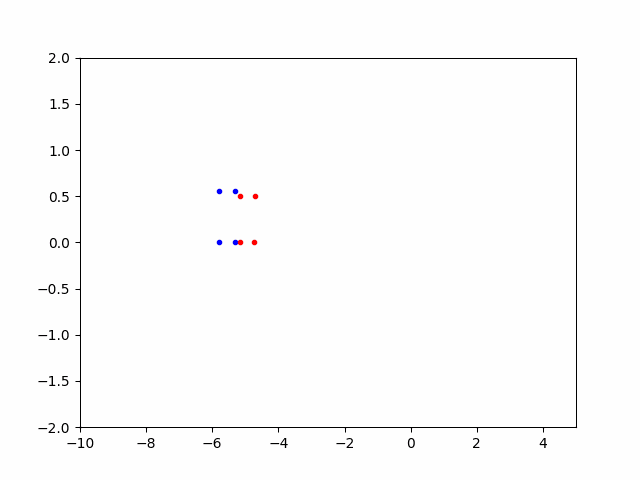
\includegraphics[scale=0.7]{sim/simi/simT1-61.png}
    \caption{Sim ohne Farbe $ v = 0.2 \cdot c$}
    \label{fig:simoF0.2}
\end{figure}

\newpage

Diese Animation stellt die ersten 100 Frames der Animation dar. Es ist dabei anzumerken, dass selbstverständlich nicht tausende $.png$s erstellt werden können nur für eine Animation. 
\vspace{0.4cm}
Diese Animation zeigt einen Ausschnitt des sich bewegenden Quaders in x-Richtung. Dabei ist anzumerken, dass wir aus der y-Richtung, nämlich vom Punkt $\begin{pmatrix} 0 \\ 10 \\ 0\end{pmatrix}$, den Quader beobachten. Somit ist unsere y-Achse eigentlich die z-Achse. Die vorderen Punkte, in blau gefärbt, zeigen die Vorderseite des Quaders und die Roten die Rückseite des Quaders. Es lässt sich erkennen, dass die roten Punkte, obwohl sie den selben Abstand zueinander haben wie die blauen, einen geringeren Abstand zu haben scheinen. Dies beschreibt genau den Effekt der Längenkontraktion. 

Im Verlauf der Animation sieht man, dass sich der Abstand zwischen Punkten immer weiter verschiebt und dass sich unser Würfel, wenn man Linien zwischen den Punkten ziehen würde, zu rotieren scheint. Nebst dem Effekt der Längenkontraktion ist die sogenannte Terrell Rotation erkennbar.

Die Terrell Rotation beschreibt die scheinbare Drehung und Krümmung eines Objekts bei relativistischen Geschwindigkeiten.

Wir sehen die rechte Seite unseres Würfels logischerweise, da wir einen ruhenden Beobachter haben und jener ein bestimmtes Sichtfeld hat und man somit die rechte oder linke Seite (abhängig von $v$) eines sich bewegenden Objekts im Verlauf der Zeit sieht. Das gleiche passiert, wenn wir an einer Ampel stehen und ein Auto sich von uns wegbewegt.

Das interessante ist nun, dass sich Beobachtungen von Objekten bei relativisitischen Geschwindigkeiten nicht exakt nach den Lorentzkontraktionen verhalten aufgrund des zuvor beschriebenen Terrell Effekts. Aufgrund der Lorentzkontraktion würde man eine Kontraktion, jedoch keine Drehung erwarten. 
Man könnte nun mutmassen, dass die Drehung aufgrund vom Zerlegungssatz, also dass jede Lorentz-Transformation aus einer Drehung gefolgt von einem Boost gefolgt von einer zweiten Drehung besteht, erklärbar ist. Die wahrgenommene Drehung und Krümmung von Objekten wird also nicht durch die Lorentzkontraktion erklärt. Die gesamte Länge eines Objekts mag sich zwar verändern aber wir nehmen dies entweder als Drehung, Streckung, Kontrahierung oder Krümmung war.
Dies kann man nicht direkt aus den Lorentz-Transformationen schlussfolgern, wenn man sich nicht an Simulationen wendet. \cite{T}
\vspace{0.4cm}
R.Penrose: "the light from the trailing part reaches the observer from behind the sphere, which it can do since the sphere is continuously moving out of its way" \cite{T}
Dieses Zitat von R.Penrose, vielleicht bekannt vom Penrose-Diagramm, sagt soviel wie: Das Licht eines hinteren Teilchens erreicht den Beobachter hinter der Kugel, dies ist möglich, da sich die Kugel ständig vom Beobachter wegbewegt.
Dies erklärt somit die vermeintliche Rotation unseres Würfels und die Tatsache, dass sich zu einem Zeitpunkt in der Animation die roten Teilchen vor den blauen Teilchen befinden. Dies bedeutet, dass wir das Licht der hinteren Teilchen empfangen, weil sich der Würfel ja von uns wegbewegt. 

Um den Terrell Effekt noch deutlicher zu zeigen werden wir nun den Geschwindigkeits-Vektor $\Vec{v} = \begin{pmatrix} 0.95 \\ 0 \\ 0\end{pmatrix}$ verwenden. Dies bedeutet, dass sich unser Objekt nun mit 95\% Lichtgeschwindigkeit bewegt.


\begin{figure}[h!]
    \centering
    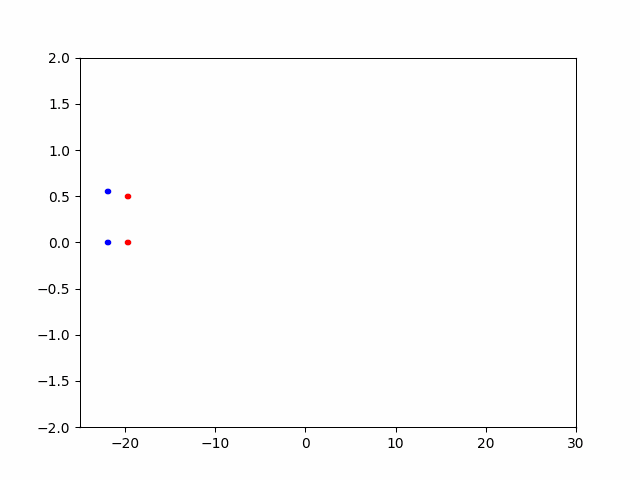
\includegraphics[scale=0.7]{sim/simi/simT2-82.png}
    \caption{Sim ohne Farbe $v = 0.95 \cdot c$}
    \label{fig:simoF0.95}
\end{figure}

Wir sehen hier nun, deutlich wie sich unser Objekt zu rotieren scheint. Der Abstand zwischen den blauen Punkten und der Abstand zwischen den roten Punkten wird deutlich verringert. Wir sehen dass der Abstand zwischen den Roten und den Blauen sich in die Länge zieht, dies zeigt eine Rotation. Wir sehen zudem eine Überlagerung der blauen und roten Punkte, dies zeigt eine Rotation um die y- bzw. z-Achse. Auch hier ist wieder die Krümmung zu erkennen. Jene sieht man an der Tatsache, dass die roten Punkte zueinander einen geringeren Abstand haben, als die Blauen.

\newpage

\begin{figure}[h!]
    \centering
    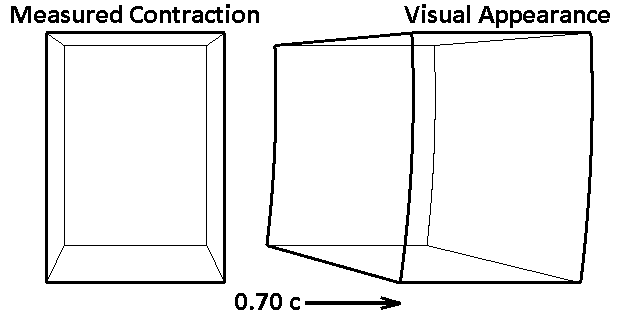
\includegraphics[scale=0.6]{sim/simi/ATRC-70.png}
    \caption{Terrell Rotation \cite{T}}
    \label{fig:ATRC}
\end{figure}

Diese Darstellung stellt genau den simulierten Würfel aus der Abbildung \ref{fig:simoF0.95} dar. Nur bewegt er sich nach rechts anstatt links. Wir sehen die erwähnte berechnete Kontraktion und das wahrgenommene Aussehen des Würfels.

\newpage

Nun wollen wir mit den selben Punkten und den selben Geschwindigkeiten eine Simulation des Würfels machen, nun aber unter der Verwendung des relativistischen Doppler-Effekts.

\begin{figure}[h!]
    \centering
    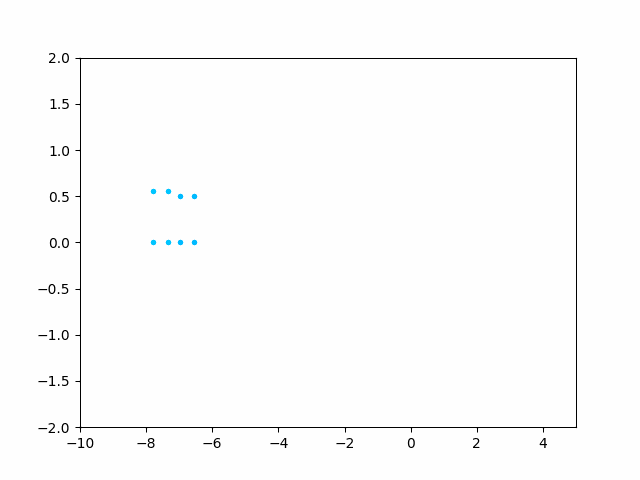
\includegraphics[scale=0.7]{sim/simi/simF1-82.png}
    \caption{Sim mit Farbe $v = 0.2 \cdot c$}
    \label{fig:simF02}
\end{figure}

Die Darstellung der Simulation entspricht \ref{fig:simoF0.2}. Der Code zur Darstellung wurde jedoch zur Abbildung des relativistischen Doppler-Effekts angepasst. Es folgt nochmals eine Erklärung des Gesehenen nun aber mit Bezug auf den relativistischen Doppler-Effekt.

Man kann in dieser Animation nun schön erkennen wie sich die Farbe unseres Quaders im Verlauf der Zeit aufgrund der zurückgelegten Distanz und Geschwindigkeit ändert. Man sieht, dass die Farbe Violett $\lambda = 400nm$ sich langsam in Richtung Blau verändert. Wenn wir nun deutlich hinschauen, können wir erkennen dass sich die vorderen Punkte des Quaders zuerst verfärben und zum Schluss der Animation auch einen helleren Blau-Ton haben als die hinteren. Diese farbliche Veränderung liegt, dem wie schon erwähnten, relativistischen Doppler-Effekt \ref{rd.1} zu Grunde. Man sieht dass bereits $geringe$ Geschwindigkeiten ($v = 0.2 \cdot c$), im Verhältnis zu relativistischen Geschwindigkeiten, einen deutlichen Einfluss auf die Wahrnehmung von Farben haben. 

Man stelle sich vor, dass sich ein Raumschiff mit $20\% c = 60'000'000 m/s$ bewegen würde. Dies sind bereits so hohe Geschwindigkeiten, dass wir uns unter ihnen gar nichts vorstellen können, da wir kein Fahrzeug mit vergleichbarer Geschwindigkeit auf der Erde haben. 

In der Simulation kommt es uns im Verhältnis zu relativistischen Geschwindigkeiten und aufgrund der Tatsache, dass wir in unserem Programm angenommen haben, dass $c = 1$ entspricht, so vor als ob sich das Objekt langsam bewegen würde. Eine andere Folge aus der Annahme, dass $c = 1$ entspricht, ist dass die Distanzen zwischen den vier Punkten des Quaders $Ls$ entsprechen. Somit haben die Punkte einen Abstand von $\approx 3 \cdot 10^8 m$. Dies entspricht ungefähr $\frac{3}{4}d_{erde-mond}$. Das bedeutet der Würfel, der vorbeifliegt riesig ist. 

In unserer Simulation sind die wahrgenommenen Zeiten im Inertialsystem der Punkte nicht dargestellt und wir können somit den Zeitenunterschied vom Beobachtersystem und Ereignissystem nicht messen und die Zeitdilatation nicht beobachten. Wir können auch hier wiederum das Phänomen der Längenkontraktion beobachten.

Wir können erkennen, dass sich die vorderen vier Punkte vor die hinteren schieben und die Längen kontrahieren. Dies ist jedoch nicht nur durch die Längenkontraktion erklärbar. Einfach gesagt braucht das Licht der vorderen Punkte, welche sich zum Zeitpunkt 0 vor den hinteren Punkten befinden, weniger lange um bei uns anzukommen und wir nehmen diese nun vor den hinteren Punkten war. Da sich das Objekt aber weiter in die linke Richtung bewegt, können wir nun den hinteren Teil des Quaders sehen. Somit lässt sich auch begründen, wieso sich die vorderen Punkte schneller bewegen und vor den hinteren Punkten die Farbe wechseln. 

Nebst der Längenkontraktion ist auch hier wieder der Terrell Effekt zu erkennen. 

Nun wollen wir den relativistischen Doppler-Effekt für unser Objekt numerisch berechnen. Wir werden allerdings die Rechnung nur für einen Punkt durchführen. Dazu verwenden wir die Gleichungen \ref{rd.1} \ref{rd.2} \ref{rd.3}. 

Unsere gegebenen Daten entsprechen: 
\begin{itemize}
    \item Ortsvektoren der Punkte
    \item Ortsvektor des Beobachters
    \item Geschwindigkeitsvektor
    \item Wellenlänge $\lambda = 400nm$
\end{itemize}

Wir nehmen einfacherheitshalber den Punkt $\Vec{x} = \begin{pmatrix} 0 \\ 0 \\ 0\end{pmatrix}$.

Zuerst müssen wir den Punkt in das Inertialsystem des Beobachters transformieren. Wir nehmen dazu an, dass $\tau = 0$ ist. $\tau = O^0$ also die Raumzeitkomponente des Beobachters. 


Wir bestimmen die euklidischen Norm des Geschwindigkeitsvektors $\Vec{v}$.

\begin{align*}
    ||\Vec{v}|| &= \sqrt{0.2^2 + 0^2 + 0^2} \\
    &= 0.2 \\
\end{align*}

Nun bestimmen wir den Lorentzfaktor $\gamma$ und das $\beta$ bestimmen. Dabei dürfen wir nicht vergessen, dass $||\Vec{v}|| = 0.2$ eigentlich $0.2 \cdot 3 \cdot 10^8 m/s$ bedeutet.

\begin{align*}
    \gamma &= \frac{1}{\sqrt{1-0.2^2}} \\
    \beta &= \frac{0.2 \cdot c}{c} = 0.2
\end{align*}

Wir boosten nun den 4er-Vektor $x = \begin{pmatrix} \lambda \\ 0 \\ 0 \\ 0\end{pmatrix}$ mit unbekannter Raumzeitkoordinate \ref{csm1}.

\begin{align*}
    x' = B(\mathbf{x}) &= \begin{bmatrix}
        \gamma & -\gamma v_x / c & -\gamma v_y / c & -\gamma v_z / c \\
        -\gamma v_x / c & 1 + (\gamma -1)\frac{{v_x}^2}{v^2} & (\gamma -1)\frac{v_x v_y}{v^2} & (\gamma -1)\frac{v_x v_z}{v^2} \\
        -\gamma v_y / c & (\gamma -1)\frac{v_y v_x}{v^2} & 1 + (\gamma -1)\frac{{v_y}^2}{v^2} & (\gamma -1)\frac{v_y v_z}{v^2} \\
        -\gamma v_z / c & (\gamma -1)\frac{v_z v_x}{v^2} & (\gamma -1)\frac{v_z v_y}{v^2} & 1 + (\gamma -1)\frac{{v_z}^2}{v^2}
    \end{bmatrix} \cdot \begin{pmatrix} \lambda \\ 0 \\ 0 \\ 0\end{pmatrix}\\
    &= \begin{bmatrix} \gamma & -0.2\gamma & 0 & 0 \\
                       -0.2\gamma & 1 + (\gamma - 1) & 0 & 0 \\
                       0 & 0 & 1 & 0 \\
                       0 & 0 & 0 & 1
        \end{bmatrix} \begin{pmatrix} \lambda \\ 0\\ 0 \\0\end{pmatrix} \\
    &= \begin{pmatrix} \gamma \lambda \\ -0.2\gamma \lambda \\ 0 \\ 0\end{pmatrix}
\end{align*}

Um unsere Gleichung \ref{csm.3} für $\tau$ aufzulösen brauchen wir die euklidische Norm des Abstandsvektors zwischen den Vektoren ohne Raumzeitkomponente.

\begin{equation*}
    d = ||\overrightarrow{ox'}|| = \sqrt{0.04{\gamma^2}{\lambda^2} + 100}
\end{equation*}

In \ref{csm.3} eingesetzt ergibt sich folgende Gleichung für $\tau$.

\begin{equation*}
    \tau = {x'}_0 + \frac{d}{c} = {x'}_0 + \sqrt{0.04{\gamma^2}{\lambda^2} + 100}
\end{equation*}

Wir können nun unsere $x'_0$ Komponente in \ref{csm.3} einsetzen und wir erhalten.

\begin{align*}
    \tau &= \gamma \lambda + \sqrt{0.04{\gamma^2}{\lambda^2} + 100} \\
    0 &= \gamma \lambda + \sqrt{0.04{\gamma^2}{\lambda^2} + 100} \\
    {\gamma^2}{\lambda^2} &= 0.04{\gamma^2}{\lambda^2} + 100 \\
    {\lambda^2} &= 100 \\
    \lambda &= 10
\end{align*}

Daraus ergibt sich folgendes für $x'$:

\begin{equation*}
    x' = \begin{pmatrix} 10.20620 \\ -2.04124 \\ 0 \\ 0\end{pmatrix}
\end{equation*}

Wir bestimmen nun des Abstandsvektor und die euklidische Norm dieses Vektors von x' ohne die Raumzeitkoordinate und O ohne die Raumzeitkoordinate. Wir erhalten folgenden Abstandsvektor zwischen $x'$ und O.

\begin{align*}
    \overrightarrow{x'O} &= \begin{pmatrix} -2.04124 \\ -10 \\ 0\end{pmatrix} \\
    ||\overrightarrow{x'O}|| &= 10.20620
\end{align*}

Nun bestimmen wir den Winkel $\theta_r$. Dazu nehmen wir jedoch an, dass sich unser Objekt mit $-||\Vec{v}||$ bewegt. Da wir uns auch in jene Richtung bewegen. Somit erhalten wir kein Werte für $\lambda$ im Infrarotbereich.

\begin{equation*}
    \theta_r = \arccos({\frac{-\Vec{v} \cdot \overrightarrow{x'O}}{||-\Vec{v}|| ||\overrightarrow{x'O}||}}) = 1.369438551
\end{equation*}

Wir können nun die empfangene Frequenz $f_r$ mit unseren berechneten Parametern bestimmen. Wir müssen jedoch zuerst noch $f_s$ bestimmen.

\begin{align*}
    f_s &= \frac{3 \cdot 10^8 m/s}{400 \cdot 10^{-7}m}\\
    f_r &= \frac{f_s}{\gamma(1 + \beta \cos{\theta_r})} \\
    &= 7.06583599 \cdot 10^{14} Hz
\end{align*}

Nun verbleibt uns nur noch die Berechnung der empfangenen Wellenlänge $\lambda_r$.

\begin{equation*}
    \lambda_r = \frac{3 \cdot 10^8 m/s}{f_r} = 425nm
\end{equation*}

Um dies für die gesamte Simulation durchzuführen, müsste man dies für jeden Punkt für alle Werte von $\tau = {1,...,100}$ wiederholen.

Zur Veranschaulichung führen wir die Simulation noch für $95\%$ Lichtgeschwindigkeit $\vec{v} = \begin{pmatrix} 0.95 \\ 0 \\ 0 \end{pmatrix}$ durch. Dazu verwenden wir dieselbe Simulation \ref{fig:simoF0.95} jedoch mit dem relativistischen Doppler-Effekt. Wir verwenden zur Abwechslung nun eine andere Farbe, namentlich Blau $\lambda = 425 nm$.

\begin{figure}[h!]
    \centering
    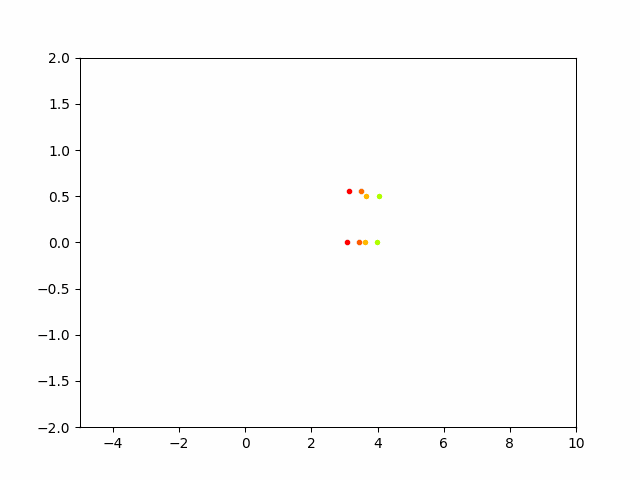
\includegraphics[scale=0.7]{sim/simi/simF2-10.png}
    \caption{Sim mit Farbe $v = 0.95 \cdot c$}
    \label{fig:sim0.95}
\end{figure}

Man sieht einen Quader, welcher mit 95\% Lichtgeschwindigkeit an uns vorbeifliegt. Wir sehen ihn immer noch aus der Perspektive von der y-Achse.
Unser Quader scheint etwas langsam zu sein für seine Geschwindigkeit. Dies ist mit Absicht, da wir den Farbverlauf bei relativistischen Geschwindigkeiten zeigen möchten.
Wir sehen, dass unser Quader zuerst unsichtbar ist und sich dann von Blau bis Rot verfärbt und dann wieder unsichtbar wird. Man sieht also schön, dass die Frequenz des Lichts höher wird, wenn wir uns mit einer höheren Geschwindigkeit bewegen.

Auch hier erkennt man die Längenkontraktion wieder, jedoch ist sie nicht lange zu erkennen, da unser Quader wieder unsichtbar wird. 
Man sieht den relativistischen Doppler-Effekt hier sehr gut. Die Farbveränderung verläuft nach dem Schema welches sich auf \cite{RD} befindet.

\newpage

\subsection{Bewegung in x-Richtung Sphäre} In diesem Abschnitt wollen wir beobachten, wie sich eine Sphäre bei relativistischen Geschwindigkeiten verhält. Da eine Sphäre aus vielen Punkten besteht, ist es zu mühsam alle von Hand zu definieren. Um es uns leichter zu machen, schreiben wir ein Programm, welches uns die Sphären-Koordinaten erträgt und wir so dann mit ihnen rechnen können.
\lstset{language=Python}
\lstset{frame=lines}
\lstset{caption={Sphäre}}
\lstset{label={lst:Sphäre}}
\lstset{basicstyle=\fontsize{11}{13}}
\begin{lstlisting}
import math


def get_sphere_coordinates(radius, center_x, center_y, center_z):

    x_coordinates = []
    y_coordinates = []
    z_coordinates = []

    num = 10
  # Berechnung der Koordinaten fuer eine Sphaere durch Iteration ueber
  # einen Bereich von Winkeln von 0 bis 2 pi im Bogenmass fuer theta und phi
    for theta in np.arange(0, math.pi, 0.7):
        for phi in np.arange(0, 2 * math.pi, 0.6):
      # Berechnung der x,y und z Koordinaten
      # x = center_x + radius * sin(phi) * cos(theta)
      # y = center_y + radius * sin(phi) * sin(theta)
      # z = center_z + radius * cos(phi)
            x = center_x + radius * math.sin(phi) * math.cos(theta)
            y = center_y + radius * math.sin(phi) * math.sin(theta)
            z = center_z + radius * math.cos(phi)
      
      
            x_coordinates.append(x)
            y_coordinates.append(y)
            z_coordinates.append(z)
  

    return x_coordinates,y_coordinates,z_coordinates


sphere_coordinates = get_sphere_coordinates(1, 1, 3, 4)

\end{lstlisting}

\newpage

\begin{figure}[h!]
    \centering
    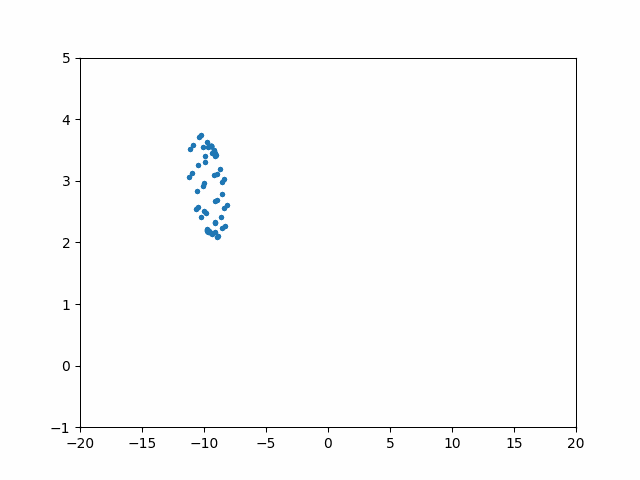
\includegraphics[scale=0.7]{sim/simso-87.png}
    \caption{Sim Sphäre v = $0.2 \cdot c$}
    \label{fig:sims0.2}
\end{figure}
Diese Abbildung zeigt eine Kugel welche sich mit 20\% der Lichtgeschwindigkeit nach links fortbewegt. Wir sehen hier auch wieder die Terrell Rotation. Nämlich sehen wir wie sich die Kugel zu drehen scheint und nicht nur aufgrund der Perspektive. Das Licht des hinteren Teilchens trifft unseren Beobachter hinter der Sphäre. Dies funktioniert, da sich unsere Sphäre bewegt. Diese Tatsache, führt dazu, dass wir eine Drehung und eine scheinbare Verzerrung sehen. Die Länge wird also visuell nicht, wie erwartet, kontrahiert sondern gestreckt und gekrümmt. 
Wie schon bei der Beschreibung der Quader-Simulation erwähnt, ist die spezielle Relativitätstheorie trotz der scheinbar falschen visuellen Darstellung richtig. Tatsächlich beobachten wir eine Kontraktion, wenn wir die Sphäre ausmessen würden. 

\newpage

Nun wollen wir zur Veranschaulichung der Terrell Rotation und Längenkontraktion bei Sphären, dasselbe Prozedere noch bei $v = 0.95 \cdot c$ wiederholen. 

\begin{figure}[h!]
    \centering
    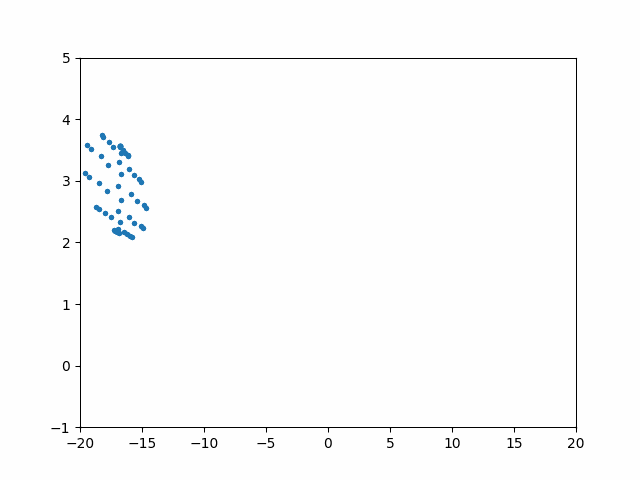
\includegraphics[scale=0.7]{sim/sims-50.png}
    \caption{Sim Sphäre v = $0.95 \cdot c$}
    \label{fig:sims0.95}
\end{figure}

Die Terrell Rotation wird hier im Vergleich zur Simulation \ref{fig:sims0.2} besser dargestellt. Dies macht auch Sinn denn der Effekt der Längenkontraktion ist bei hohen Geschwindigkeiten und weiter Entfernung drastischer als bei geringeren Geschwindigkeiten. Wir können hier nun im Vergleich zur letzten Simulation erkennen, dass sich unsere Sphäre krümmt und auseinander dehnt, da wir uns mit hohen Geschwindigkeiten bewegen.


\newpage

Es folgt wiederum eine Animation zur Terrell Rotation von sphärischen Körpern.

\begin{figure}[hb]
    \centering
    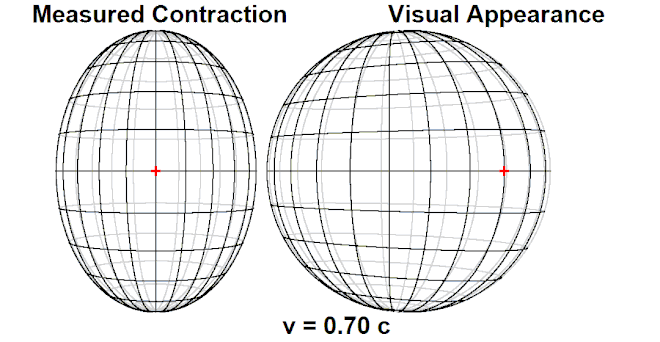
\includegraphics[scale=0.6]{sim/simi/ARTS-70.png}
    \caption{Terrell Rotation Sphäre}
    \label{fig:TRS}
\end{figure}

Diese Animation verdeutlicht die Streckung unserer animierten Sphäre. Man sieht, dass sie sich bei geringen Geschwindigkeiten, die Sphäre leicht dreht und je höher die Geschwindigkeit ist, desto stärker dreht und krümmt sich die Sphäre. Wie schon erwähnt ist die gemessene Länge mittels Lorentzkontraktion beweisbar, jedoch sehen wir visuell etwas anderes.


\newpage

\subsection{Bewegung in x-Richtung Licht-Uhr} mit mehreren bewegten Teilchen im Inertialsystem $S$. Es folgt eine Simulation, welche Licht in einem Zug darstellt. Diese Simulation verdeutlicht die in \ref{simult}, \ref{RT},\ref{ZD} und \ref{LK} etablierte Gleichzeitigkeit, Zeitdilatation und Längenkontraktion. 

\begin{figure}[h!]
    \centering
    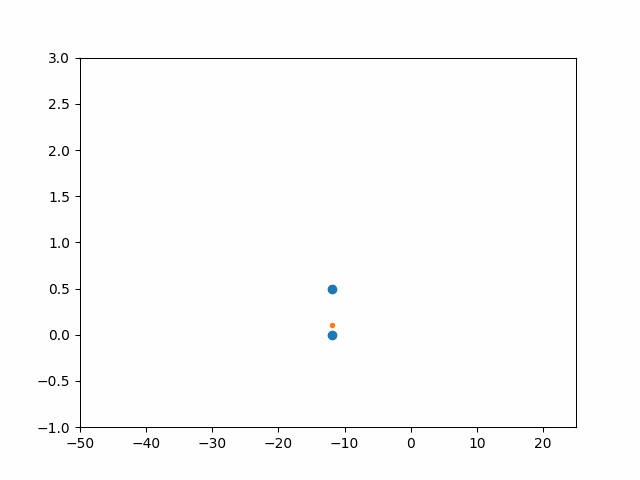
\includegraphics[scale=0.7]{sim/simLT-28.png}
    \caption{Sim Licht im Zug v = $0.95 \cdot c$}
    \label{fig:simLT0.95}
\end{figure}

Man nennt diese Simulation auch $Licht-Uhr$, da unser Licht-Teilchen hin und her springt wie im Sekundentakt.
Die Simulation dient zur Veranschaulichung des in \ref{RT} beschriebenen Effekts der Relativität der Zeit und der daraus folgenden Zeitdilatation. 
Unser System ist folglich gleich aufgebaut wie in \ref{RT}. 
Die blauen Punkte stellen die beiden Spiegel dar an welchen das Licht reflektiert wird. Wir sind in diesem Fall Sam, der Beobachter, welcher das System von $\begin{pmatrix} 0 \\ 10 \\ 0\end{pmatrix}$ aus betrachtet. Wir sehen hier schön wie das Licht aufgrund der Geschwindigkeit einen zickzackförmigen Verlauf hat und wenn wir uns vorstellen, dass wir im Ereignissystem wären, würden wir das Licht sich nur nach oben und unten bewegen sehen. Man sieht also dass die Gleichungen \ref{egn: t 1.1} wahr sein müssen. Es vergeht somit auch, aus Sams Perspektive, mehr Zeit bis das Licht nach oben oder nach unten geht.

\newpage

Zur Illustration folgt nun eine Grafik in welcher der Weg des Lichts dargestellt wird.

\begin{figure}[h!]
    \centering
    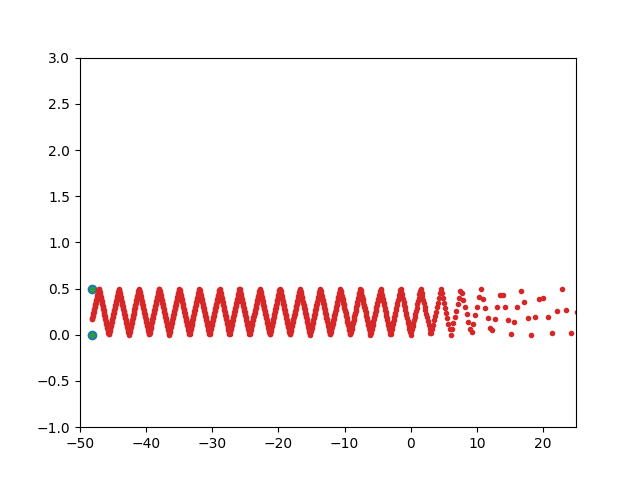
\includegraphics{simLCP.png}
    \caption{Weg des Lichts}
    \label{fig:wol}
\end{figure}

Man sieht hier schön anhand der Zickzacklinie, dass das Licht einen längeren Weg braucht aus der Sicht vom Beobachtersystem.

\newpage

\subsection{Bewegung in y-Richtung} Wir wollen nun dasselbe Spiel für die y-Richtung machen, da dieselben Gesetzmässigkeiten auch hier gelten, wird hier nicht im Detail auf das Geschehene eingegangen. 
Es folgt eine Simulation der Bewegung eines Quaders und einer Sphäre in y-Richtung.
Wir nehmen wiederum an, dass unser Würfel dieselben Koordinaten wie zuvor hat. Nun bewegt er sich allerdings mit dem Geschwindigkeitsvektor $\Vec{v} = \begin{pmatrix} 0 \\ 0.2 \\ 0\end{pmatrix}$ in y-Richtung fort. Zusätzlich nehmen wir noch an, dass unser Objekt eine Farbe mit der Wellenlänge $\lambda=400nm$ also Violett hat.

\begin{figure}[h!]
    \centering
    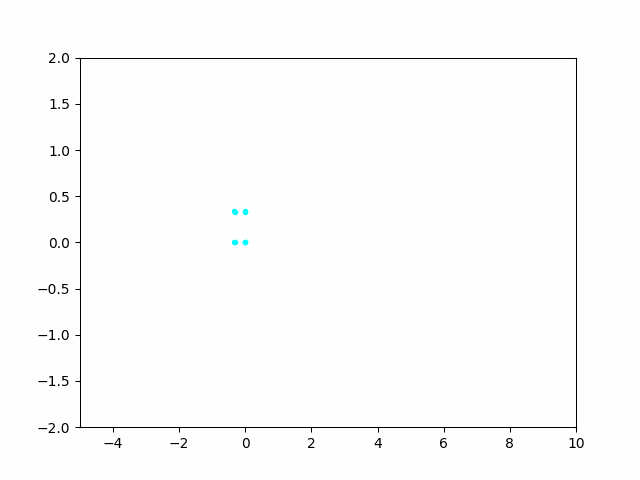
\includegraphics[scale=0.7]{sim/simi/simy02-38.png}
    \caption{Sim in y-Richtung $v = 0.2 \cdot c$}
    \label{fig:simy02}
\end{figure}

Wir sehen hier schön wie sich unser Würfel nach hinten bewegt, aufgrund dessen, dass wir als Beobachter auf der y-Achse stehen. Der relativistische Doppler-Effekt ist ebenfalls erkennbar, er verändert sich jedoch im Verlauf der Simulation nicht.  Dies scheint der Fall zu sein, da $\theta = 0$ ist. 
Wir sehen hier auch praktisch keine Längenkontraktion. Man erkennt auch keine Terrell-Rotation, vermutlich da sich unser Ereignis entlang derselben Achse bewegt, auf welcher sich unser Beobachter befindet.

Es macht keinen Sinn dasselbe für höhere Geschwindigkeiten darzustellen, da sich aus empirischen Versuchen ergeben hat, dass man nichts sieht. Ab der Geschwindigkeit $v = 0.5 \cdot c$ ist nichts mehr zu erkennen, da wir uns ab dann im infraroten Bereich befinden und wir solche Wellenlängen mit dem menschlichen Auge nicht sehen können. Man beobachtet einfach eine graduelle Farbveränderung je höher die Geschwdindigkeit ist, jedoch keine Veränderung während dem Verlauf der Simulation. Dies zeigt eigentlich schön den sogenannten \emph{Red-Shift} mit welchem wir Objekte und unser Universum selbst datieren können.

\newpage


\section{Fazit}
\paragraph{Rückblick}
Wie man sieht lässt sich mit unserem Programm eine zahlreich Anzahl von Ereignissen grafisch darstellen. Seien es Ereignisse bei langsamen Geschwindigkeiten oder solche bei hohen Geschwindigkeiten. Wir können die verschiedenen Effekte der speziellen Relativitätstheorie nun visuell deuten und können nun näherungsweise verstehen, was für Prozesse in unserem Universum verrichtet werden.
Eine wichtige Erkenntnis aus der Arbeit ist, dass man den mathematischen Grundlagen nicht immer vollkommen trauen kann. Dies sieht man deutlich beim Terrell Effekt. 
Was ein anderer wichtiger Schluss aus dieser Arbeit ist, dass Programmieren einen grossen Teil der Arbeit im physikalisch-mathematischen Bereich darstellt und die meisten Erkenntnisse ohne jene nicht möglich wären und dass ohne die Arbeit von früheren Wissenschaftlern wie Einstein Erkenntnisse der modernen Wissenschaften nicht möglich wären.

\paragraph{Ausblick} 
Was hätte man noch tun können, wenn man mehr Zeit gehabt hätte? Ich hätte vermutlich den Code noch etwas optimiert, um die Berechnungsdauer, welche eigentlich durchaus schnell ist für die ganzen Operationen, zu verringern. Ausserdem hätte ich, wie in der Einführung schon erwähnt, etwas zur Schwarzschildmetrik machen wollen. Ich hätte sicherlich noch eine Simulation eines schwarzen Lochs eingefügt. Dazu bräuchte man jedoch, wenn man es genau nehmen möchte, die generelle Relativitätstheorie, da sich die spezielle Relativitätstheorie auf die flache Raumzeit bezieht und somit eigentlich eine einfache Metrik hat. Welche sich bei der generellen Relativitätstheorie verändern würde. Die spezielle Relativitätstheorie beinhaltet somit Gravitation nicht als Konzept, da Gravitation aus der generellen Relativitätstheorie geschlossen werden kann, aufgrund der gekrümmten Raumzeit. Es wäre vermutlich sicher auch spannend gewesen ein Experiment beim CERN machen zu dürfen, welches jedoch unwahrscheinlich ist, aufgrund dessen dass es sich hierbei um eine Maturaarbeit handelt. Man hätte bspw. das Michelson-Morley Experiment wiederholen können und so die Lorentz Invarianz vom elektromagnetischen Feld zeigen können.

\section{Danksagung}
Zuallererst bedanke ich mich bei den Personen der Wissenschaft, welche mich zu einem Thema in der theoretischen Physik inspiriert haben.
\vspace{0.4cm}
Bei Herrn Röthlisberger möchte ich mich zunächst für das Akzeptieren meiner Arbeit bedanken, da ich anfangs Probleme hatte einen Lehrer zu finden.
\vspace{0.4cm}
Da ich mir zu Beginn ein sehr komplexes Thema ausgesucht hatte, war ich sehr froh, dass Herr Röthlisberger mich auf den Boden der Realität zurückgeholt hat. Und mir daher empfohlen hat, zuerst etwas über die spezielle Relativitätstheorie zu erarbeiten, was sich als sehr gute Empfehlung rausstellte, da es dann schlussendlich doch nicht soviel Zeit zur Verfügung hatte als ich mir vorstellte.
\vspace{0.4cm}
Seine fortwährende Unterstützung im Verlauf des Projekts schätzte ich sehr, ohne ihn wäre es nicht möglich gewesen, das Programm so ansprechend zu gestalten. Bei Problemen konnte er mir immer helfen und gab mir auch dementsprechend ausführliche Erklärungen dazu.
\vspace{0.4cm}
Das umfassende Wissen von Herrn Röthlisberger half mir immer wieder weiter, sei es beim Durchschauen des Codes, wo wir zum Beispiel gemeinsam Lösungen für Probleme in der Struktur des Codes fanden, oder mit zahlreichen Hinweise zu Scripts und Webseitenlinks, die er immer für mich parat hatte.
\vspace{0.4cm}
Bei unseren gemeinsamen Treffen wuchs mein Verständnis für die spezielle Relativitätstheorie, dieses Verständnis musste ich zuerst erarbeiten, um das zugehörige Programm realisieren zu können.
\vspace{0.4cm}
Zum Schluss danke ich ihm nochmal für die viele Zeit, die er investiert hat, sowie für die Hinweise auf sachliche Fehler meinerseits.
\vspace{0.4cm}
Ebenfalls bedanke ich mich bei meinem Vater für seine Unterstützung.
\vspace{0.4cm}
Und dann möchte ich noch eine allgemeine Danksagung an alle Universitäten und Hochschulen aussprechen, die ihre Vorlesungen und Information zum Teil auf Kanäle wie YouTube einer breiten Öffentlichkeit zur Verfügung stellen.

\newpage

\listoffigures

\lstlistoflistings

\newpage

\section{Referenzen}
\bibliography{Bib}
\begin{thebibliography}{9}

\bibitem{University Physics} Hugh D. Young, Roger A. Freedman. 17.07.2015. Sears \& Zermansky's University Physics with Modern Physics. 14th Edition. Chapter 37. Relativity; p.1242.

\bibitem{Principles of Physics} Jearl Walker, David Halliday, Robert Resnick. 17.06.2014. Principles of Physics. 10th Edition. Chapter 37. Relativity; p.1008.

\bibitem{Univie Spezielle Relativittstheorie} Spezielle Relativitätstheorie. Franz Embacher. Universität Wien; [abgerufen 7.1.23]. https://homepage.univie.ac.at/franz.embacher/SRT/.

\bibitem{Vektor} Vektor. zuletzt verändert  21.12.2022. Wikipedia; [abgerufen 7.1.23]. https://de.wikipedia.org/wiki/Vektor.

\bibitem{Euclidean vector} Euclidean . zuletzt verändert  3.12.2022. Wikipedia; [abgerufen 7.1.23]. $https://en.wikipedia.org/wiki/Euclidean_vector$

\bibitem{Skalarprodukt} Euclidean . zuletzt verändert  20.12.2022. Wikipedia; [abgerufen 8.1.23]. https://de.wikipedia.org/wiki/Skalarprodukt

\bibitem{Michelson Morley} Michelson Morley.zuletzt verändert  15.12.2022. Wikipedia; [abgerufen 7.1.23]. https://de.wikipedia.org/wiki/Michelson-Morley-Experiment

\bibitem{Inertialsystem} Inertialsystem. Copyright 1998 Spektrum Akademischer Verlag, Heidelberg; [abgerufen 6.1.23]. https://www.spektrum.de/lexikon/physik/inertialsystem/7224.

\bibitem{Minkowski Space} What Is Minkowski Space?. BYJUS [abgerufen 14.1.23].https://byjus.com/physics/minkowski-space/

\bibitem{Minkowski Diagrams} Joel C. Corbo. 17.03.2008. Supplementary Lecture I: Spacetime Diagrams and Causality. 

\bibitem{GT1} Galilei-Transformation. de-academic; [zuletzt abgerufen 9.10.22]. https://de-academic.com/dic.nsf/dewiki/492274.

\bibitem{GT2} The Galilean Transformation. psi.phys. Simon Connell. 21.02.2006; [zuletzt abgerufen 22.12.22]. $http://psi.phys.wits.ac.za/teaching/Connell/phys284/2005/lecture-01/lecture_01/node5.html.$

\bibitem{GT3} Galilean-Transformation. BYJUS [abgerufen 10.10.22].https://byjus.com/physics/galilean-transformation/.

\bibitem{GT4} Galilean invariance. zuletzt verändert 7.01.2023. Wikipedia; [abgerufen 10.10.2022]. $https://en.wikipedia.org/wiki/Galilean_invariance$

\bibitem{GT5} Is time an invariant of Galilean transformation?. Stackexchange. 22.06.2019. https://physics.stackexchange.com/questions/487442/is-time-an-invariant-of-galilean-transformation

\bibitem{4erV} Bewegungsgleichung der speziellen Relativitätstheorie. WaBis.Dienstag, 26. Juni 2012; [abgerufen 15.1.23]. http://walter.bislins.ch/blog/index.asp?page=Bewegungsgleichung+der+speziellen+Relativit%E4tstheorie.

\bibitem{LT1} Allgemeine Mechanik HS 16. G.M. Graf. ETH Zürich. Kapitel 9: Relativistische Mechanik.

\bibitem{RD} Relativistic Dopplereffect. zuletzt verändert 23 Oktober 2022. [abgerufen 21.1.23]. $https://en.wikipedia.org/wiki/Relativistic_Doppler_effect$

\bibitem{T} Terrell Rotation. zuletzt verändert 8.11.2022. [abgerufen 26.1.23]. $https://en.wikipedia.org/wiki/Terrell_rotation$

\bibitem{LA} Lineare Algebra. TH-Nürnberg. https://www.th-nuernberg.de/fileadmin/fakultaeten/amp/Stry/kapitel5.pdf

\bibitem{Elementary Linear Algebra} Howard Anton, Chris Rorres. 15.03.2010. Elementary Linear Algebra with Supplemental Applications.

\bibitem{Wikipedia Determinant} Determinant. zuletzt verändert 13.01.2023. [abgerufen 15.1.23]. https://en.wikipedia.org/wiki/Determinant

\bibitem{Metrik ED} Euklidische Distanz. Studyflix. https://studyflix.de/mathematik/euklidische-distanz-1972

\bibitem{SO} Stackoverflow. https://stackoverflow.com/

\bibitem{SE} Stackexchange. https://physics.stackexchange.com

\end{thebibliography}



\end{document}